\documentclass[12pt,a4paper,oneside]{report}

% ---- Packages ----
\usepackage[utf8]{inputenc}
\usepackage[T1]{fontenc}
\usepackage{times}
\usepackage[margin=1in]{geometry}
\usepackage{setspace}
\usepackage{graphicx}
\usepackage{booktabs}
\usepackage{longtable}
\usepackage{array}
\usepackage{multirow}
\usepackage{caption}
\usepackage{subcaption}
\usepackage{amsmath,amssymb}
\usepackage{algorithm}
\usepackage{algpseudocode}
\usepackage{listings}
\usepackage{hyperref}
\usepackage{url}
\usepackage{titlesec}
\usepackage{fancyhdr}
\usepackage{tocloft}
\usepackage{float}
\usepackage{enumitem}
\usepackage{xcolor}
\usepackage{tikz}
\usetikzlibrary{positioning,shapes.geometric,arrows.meta}

% ---- Page setup (matching original NIT Patna thesis) ----
\sloppy
\onehalfspacing
\setlength{\parindent}{0.5in}
\setlength{\parskip}{0pt}

% ---- Chapter/Section formatting (matching original) ----
\titleformat{\chapter}[display]
  {\normalfont\bfseries\centering\Large}
  {\MakeUppercase{\chaptertitlename}\ \thechapter}{0pt}
  {\Large\MakeUppercase}
\titlespacing*{\chapter}{0pt}{0pt}{20pt}

\titleformat{\section}
  {\normalfont\bfseries}{\thesection}{1em}{}
\titleformat{\subsection}
  {\normalfont\bfseries}{\thesubsection}{1em}{}

% ---- TOC/LOF/LOT formatting (colon after figure/table number) ----
\renewcommand{\cftfigpresnum}{Figure }
\renewcommand{\cftfigaftersnum}{:}
\setlength{\cftfignumwidth}{6em}
\renewcommand{\cfttabpresnum}{Table }
\renewcommand{\cfttabaftersnum}{:}
\setlength{\cfttabnumwidth}{5.5em}

% ---- Header/Footer ----
\pagestyle{fancy}
\fancyhf{}
\fancyfoot[C]{\thepage}
\renewcommand{\headrulewidth}{0pt}

% ---- Listings style for code/JSON ----
\lstset{
  basicstyle=\small\ttfamily,
  breaklines=true,
  frame=single,
  numbers=none,
  captionpos=b,
}

% ---- Hyperref setup ----
\hypersetup{
  colorlinks=true,
  linkcolor=black,
  citecolor=black,
  urlcolor=blue,
}

% ---- Figure path ----
\graphicspath{{figures/}{../results/figures/}}

\begin{document}

% ====================================================================
% TITLE PAGE
% ====================================================================
\begin{titlepage}
\centering
\vspace*{1cm}

{\Large\bfseries
\begin{spacing}{1.2}
\centering
ENHANCING HEALTHCARE INSURANCE FRAUD\\[3pt]
DETECTION AND PREVENTION WITH A MACHINE\\[3pt]
LEARNING AND BLOCKCHAIN-BASED APPROACH
\end{spacing}
}

\vspace{1.5cm}
{\large\bfseries A Dissertation}

\vspace{0.5cm}
Submitted in Partial Fulfilment of the Requirements for\\
the Award of the Degree of

\vspace{0.5cm}
{\large\bfseries Integrated Master of Science}\\
\textit{In}\\
{\large\bfseries Mathematics}

\vspace{1cm}
\textit{Submitted by}\\
{\large\bfseries Dubasi Pavan Kumar}\\
Roll No. 1909012, Enrolment No. 190616

\vspace{1cm}
\textit{Under the Supervision of}\\
{\large\bfseries Dr. Rajesh Kumar Sinha}\\
Assistant Professor

\vspace{1cm}

\includegraphics[width=3cm]{nitp-logo.png}

\vspace{0.5cm}
{\large\bfseries Department of Mathematics}\\
NATIONAL INSTITUTE OF TECHNOLOGY PATNA\\
PATNA -800005\\
{\large\bfseries January to June, 2024}
\end{titlepage}

% ====================================================================
% FRONT MATTER
% ====================================================================
\pagenumbering{roman}

% ---- CERTIFICATE ----
\newpage
\begin{center}
{\Large\bfseries CERTIFICATE}
\end{center}

\vspace{2cm}

This is to certify that \textbf{Mr. Dubasi Pavan Kumar}, with \textbf{Roll No. 1909012} and \textbf{Enrollment No. 190616}, is registered for the Integrated Master of Science Programme in the Department of Mathematics at the National Institute of Technology Patna.

\vspace{1.5cm}

I hereby recommend that the Dissertation entitled ``\textbf{Enhancing Healthcare Insurance Fraud Detection And Prevention With A Machine Learning And Blockchain-based Approach}'' be accepted as partial fulfillment of the requirements for evaluation and award of the Integrated Master of Science degree by the National Institute of Technology Patna.

\vspace{4cm}

\noindent
\begin{minipage}[t]{0.45\textwidth}
\rule{5cm}{0.5pt}\\
Dr. Rajesh Kumar Sinha\\
Assistant Professor\\
Department of Mathematics\\
National Institute of Technology, Patna
\end{minipage}
\hfill
\begin{minipage}[t]{0.45\textwidth}
\raggedleft
\rule{5cm}{0.5pt}\\
Dr. Rishi Kumar Jha\\
Head of the Department\\
Department of Mathematics\\
National Institute of Technology Patna
\end{minipage}

% ---- DECLARATION ----
\newpage
\begin{center}
{\Large\bfseries DECLARATION AND COPYRIGHT TRANSFER}
\end{center}

\vspace{1cm}

I, Dubasi Pavan Kumar, Roll No. 1909012, and Enrolment No. 190616, am a registered candidate for the Integrated Master's Programme under the Department of Mathematics at the National Institute of Technology Patna. I hereby declare that the work presented in this Dissertation is my own original work and does not contain any material for which the copyright belongs to a third party. Furthermore, I confirm that this work has not been presented, and will not be presented, to any other University/Institute for a similar or any other degree award.

I further confirm that for all third-party copyright material in my Major Project (including any electronic attachments), I have ``blanked out'' third party material from the copies of the thesis/dissertation/book/articles etc; fully referenced the deleted materials and where possible, provided links (url) to electronic sources of the material.

I hereby transfer exclusive copyright for this Major Project to National Institute of Technology Patna. The following rights are reserved by the author:

\begin{enumerate}[label=\alph*)]
\item The right to use, free of charge, all, or part of this article in my future work, such as books and lectures, giving reference to the original place of publication and copyright holding.
\item The right to reproduce the article or thesis for my own purpose, provided that the copies are not offered for sale.
\end{enumerate}

\vspace{2cm}

\noindent
\rule{5cm}{0.5pt}\\
Dubasi Pavan Kumar\\
Roll No. 1909012\\
Integrated Master of Science\\
Department of Mathematics\\
Date:

% ---- COPYRIGHT NOTICE ----
\newpage
\begin{center}
\vspace*{3cm}
{\Large\bfseries COPYRIGHT NOTICE}
\end{center}

\vspace{2cm}

\begin{center}
Copyright \textcopyright\ 2024 by NIT Patna. All rights reserved.
\end{center}

\vspace{1cm}

No part of this publication may be reproduced, distributed, or transmitted in any form or by any means, including photocopying, recording, or other electronic or mechanical methods, without prior written permission, except in the case of brief quotations embodied in critical scholarly reviews, and other non-commercial uses with an acknowledgment/reference permitted by copyright law.

% ---- ACKNOWLEDGMENT ----
\newpage
\begin{center}
{\Large\bfseries ACKNOWLEDGMENT}
\end{center}

\vspace{1cm}

\hspace{0.5in}I am deeply grateful to my supervisor, Dr. Rajesh Kumar Sinha, for his invaluable guidance, feedback, and engagement throughout the development of this project. His expertise and insights have been instrumental in shaping my work and ensuring its success.

\hspace{0.5in}I would also like to extend my sincere appreciation to my colleagues and family members, who generously offered their time and expertise to support me in this endeavor. Their collaboration and encouragement have been vital in bringing this project to fruition.

\hspace{0.5in}I am grateful to Dr. Rishi Kumar Jha, Associate Professor \& Head of the Department of Mathematics at the National Institute of Technology Patna, for his cooperation and for providing all the necessary resources and facilities for the completion of this project.

\hspace{0.5in}Lastly, I would like to express my heartfelt gratitude to my parents and all faculty members of the Department of Mathematics for their constant support, encouragement, and belief in me throughout this journey. Their unwavering support has been my source of strength and inspiration.

% ---- DEDICATION ----
\newpage
\vspace*{5cm}
\begin{center}
\textit{This Dissertation is wholeheartedly dedicated to my friends\\
Vilas Choudhury, Billa Sujith, Vikram Patil who have provided unwavering\\
motivation and steadfast support throughout this academic journey.}
\end{center}

% ---- ABSTRACT ----
\newpage
\begin{center}
{\Large\bfseries ABSTRACT}
\end{center}

\vspace{1cm}

\hspace{0.5in}The recent global digital revolution has profoundly impacted the healthcare industry, prompting an in-depth exploration of how AI, cloud computing, and blockchain technology can enhance healthcare systems. This study specifically focuses on the rising issue of healthcare insurance fraud and how the combination of machine learning (ML) and blockchain technology offers a robust solution. The research delves into various fraud detection methodologies, including supervised and unsupervised learning, mixed methods, and blockchain-based solutions. It highlights the critical importance of security and privacy issues in healthcare apps, such as maintaining patient confidentiality, verifying user identities, and ensuring data integrity.

\hspace{0.5in}The study investigates the effectiveness of blockchain-based systems and ML classifiers, including XGBoost, LightGBM, CatBoost, Gradient Boosting, Random Forest, and a weighted ensemble method, in detecting healthcare fraud. The approach involves aggregating 558,211 Medicare claims into 5,410 provider-level records with 190 engineered features, applying Optuna-tuned hyperparameters with 10-fold stratified cross-validation, and securing prediction records through ECIES encryption (secp256k1 + AES-256-GCM) on a SHA-256 blockchain with Merkle tree integrity verification.

\hspace{0.5in}The results demonstrate that a weighted ensemble of the five Optuna-tuned tree-based classifiers achieves the best F1-score of 0.7345 at a fixed threshold of $t=0.444$, with a precision of 73.7\% and recall of 74.7\%. A notable finding is that SMOTE-ENN synthetic oversampling consistently degrades performance by 7 to 10 percent, with native cost-sensitive class weighting proving superior for this imbalanced dataset. SHAP and LIME explainability analyses identify deductible payment patterns, maximum reimbursement amounts, and claim duration anomalies as the strongest fraud indicators.

\hspace{0.5in}In conclusion, the dissertation evaluates the real-world implications of the proposed approach, emphasizing its potential to significantly streamline fraud detection within the healthcare insurance ecosystem through the integration of interpretable machine learning and cryptographically secure audit trails.

\vspace{1cm}

\noindent\textbf{Keywords:} Healthcare Fraud, Machine Learning, Blockchain, ECIES Encryption, XGBoost, SHAP, LIME, Optuna, SMOTE-ENN, Ensemble Models, Provider-Level Fraud Detection, Merkle Tree, SHA-256, Cost-Sensitive Learning.

% ---- TABLE OF CONTENTS ----
\newpage
\tableofcontents

\newpage
\listoffigures

\newpage
\listoftables

% ====================================================================
% MAIN CONTENT (modular chapter inputs)
% ====================================================================
\newpage
\pagenumbering{arabic}

\chapter{Introduction}

% ====================================================================
\section{Overview}
% ====================================================================

In recent years, digital transformation has expanded to become a truly global phenomenon. Traditional systems in industries such as education, finance, and healthcare are being upgraded with the adoption of artificial intelligence (AI), cloud computing, and blockchain technology \cite{zhang2021}. The term \textit{smart healthcare} refers to the systematic incorporation of electronic means into medical treatment. Using Electronic Health Records (EHRs), mobile internet, wearable technology, and other connected health infrastructure, remote patient monitoring entails collecting, storing, and analysing relevant patient data in real time. The insights gained from continuous monitoring can be used for more accurate illness detection, proactive disease management, and preventive intervention. As a direct consequence, healthcare providers gain the capacity to deliver more personalised, efficient, and timely care to their patients while simultaneously reducing the administrative burden associated with traditional paper-based record systems \cite{tian2019,mohanty2016}.

Despite its many advantages, smart healthcare introduces a set of challenges that remain to be resolved before these systems can reach their full potential. Security and privacy concerns, bandwidth constraints, and latency issues are prominent among these difficulties. Spoofing, cloud polling, radio-frequency (RF) jamming, and Denial-of-Service (DoS) attacks are some of the threats that can befall devices used in smart healthcare networks. Data transmissions frequently traverse networks operated by third parties, increasing exposure to interception and manipulation. These vulnerabilities can endanger both medical facilities and individual patients \cite{zeadally2020}. Electronic health records are particularly susceptible to a wide range of security threats because they contain sensitive personal and clinical information. If such information were to be leaked or tampered with, patients' well-being could be severely jeopardised. A breach of this nature might lead to serious consequences - for example, an attacker posing as a legitimate patient to gain access to medical records or altering prescribed treatments in ways that cause direct physical harm \cite{alomar2021}.

% ====================================================================
\section{Healthcare Insurance}
% ====================================================================

A health insurance policy, commonly abbreviated as HI, is a contractual agreement between an insurance provider and a policyholder whereby the insurer undertakes to cover specified medical costs incurred by the insured party. Losses arising from accidents, hospitalisation, incapacity, unintentional injury, and related damages are among the categories that HI can help compensate for, as broadly defined by the Health Insurance Association of America \cite{healthinsurance2021}. Policyholders are required to make regular premium payments in exchange for this coverage. The insurance entity may be a private commercial company or a government-operated public agency. The persistently rising cost of healthcare services has made health insurance an increasingly essential financial product for modern consumers, with additional incentives provided by the tax advantages that accompany many HI schemes \cite{sheshasaayee2018}. Historically, filing a Health Insurance Claim (HIC) required policyholders to visit an insurance office in person during restricted business hours, complete voluminous forms manually, and then await a response regarding their claim status - a process both inefficient and prone to human error. This reliance on paper-based workflows and manual human resources made HIC audits disproportionately labour-intensive.

The digitalisation of healthcare insurance processes has yielded substantial improvements in efficiency, transparency, and accountability. Maintaining and integrating paper-based health claim records was a complex and time-consuming undertaking that introduced multiple points of failure and opportunities for data manipulation. Digital systems, by contrast, offer the following key advantages:

\begin{enumerate}[label=\roman*.]
    \item \textbf{Reduced processing time:} Claims can be submitted, validated, and adjudicated electronically within hours rather than days or weeks.
    \item \textbf{Lower administrative costs:} Automation of routine processing tasks reduces the need for large clerical workforces, cutting overhead.
    \item \textbf{Improved accuracy:} Automated data validation reduces transcription errors and inconsistencies inherent in manual data entry.
    \item \textbf{Greater transparency:} Digital audit trails allow regulators, providers, and policyholders to trace the full lifecycle of any claim.
    \item \textbf{Enhanced accessibility:} Online portals and mobile applications enable policyholders to submit claims, track status, and access policy information at any time and from any location.
    \item \textbf{Better integration:} Digital platforms facilitate seamless exchange of information among hospitals, diagnostic laboratories, pharmacies, and insurers, reducing duplication and improving care coordination.
\end{enumerate}

Despite these benefits, digitisation has also introduced new attack surfaces for fraudulent actors who exploit the scale, speed, and complexity of digital claims processing systems to perpetrate healthcare fraud with greater sophistication than was previously possible \cite{patil2014}.

% ====================================================================
\section{Healthcare Fraud}
% ====================================================================

In the healthcare sector, the term \textit{healthcare fraud} refers to any instance of intentional, unlawful deceit or misrepresentation of information carried out with the intent to obtain an illicit financial advantage. It encompasses a broad range of illegal actions undertaken to improperly receive healthcare funds, goods, or services from government healthcare programs, private health insurers, or individual patients. The negative consequences of healthcare fraud are wide-ranging and include higher overall healthcare expenditures for all participants in the system, diminished quality of treatment for genuine patients, and significant financial losses for both healthcare providers and publicly funded healthcare programs \cite{macfarlane2020}.

There are many distinct categories of HI fraud, and several different parties are typically involved in any given fraud scheme. Broadly, three principal actors are implicated. First, healthcare service providers - comprising physicians, hospitals, ambulance services, and diagnostic centres - who may misrepresent or fabricate the services rendered. Second, HI subscribers such as individual patients and their employers, who may provide false information at the point of enrolment or at the time of making a claim. Third, HI providers themselves - including private insurance companies and public health agencies - who may engage in unfair denial of legitimate claims, policy misrepresentation, or premium manipulation \cite{duman2017}. Figure~\ref{fig:fraud_types} presents a taxonomic overview of the principal categories of health insurance fraud.

% -------------------------------------------------------
% Figure 1.2 -- Types of Health Insurance Frauds (TikZ)
% -------------------------------------------------------
\begin{figure}[H]
\centering
% TikZ tree diagram: Types of Health Insurance Fraud
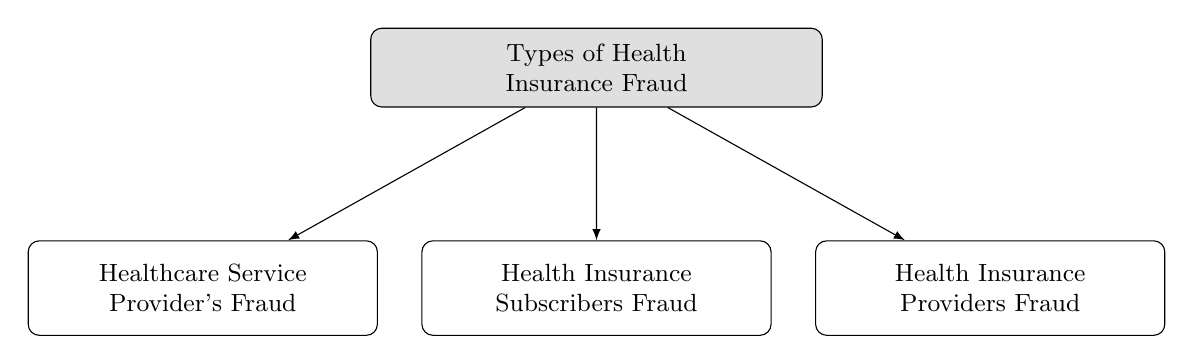
\begin{tikzpicture}[
    every node/.style={draw, rounded corners, align=center, font=\small},
    root/.style={fill=gray!25, text width=5.5cm, minimum height=1cm},
    child/.style={fill=white, text width=4.2cm, minimum height=1.2cm},
    level 1/.style={sibling distance=5cm, level distance=2.8cm},
    edge from parent/.style={draw, -latex}
]
\node[root] {Types of Health\\Insurance Fraud}
    child { node[child] {Healthcare Service\\Provider's Fraud} }
    child { node[child] {Health Insurance\\Subscribers Fraud} }
    child { node[child] {Health Insurance\\Providers Fraud} };
\end{tikzpicture}
\caption{Types of Health Insurance Fraud}
\label{fig:fraud_types}
\end{figure}

% -------------------------------------------------------
\subsection{Healthcare Service Provider's Fraud}
% -------------------------------------------------------

Healthcare service provider fraud involves deliberate misrepresentation or fabrication of clinical activities by those responsible for delivering medical care. Common manifestations include billing for services that were never rendered, upcoding - whereby a provider submits a claim for a more expensive service or procedure than was actually performed, unbundling - the practice of billing separately for component procedures that should be billed together at a lower aggregate cost, and duplicate billing for the same service across multiple claims submissions \cite{kose2015}. Providers may also engage in phantom billing, where services are invoiced on behalf of patients who do not exist or who were not present. More elaborate schemes involve kickback arrangements in which providers accept or pay referral fees in exchange for steering patients toward particular tests, treatments, or facilities regardless of clinical need. The financial incentives embedded in fee-for-service reimbursement structures create a systemic vulnerability that sophisticated fraudsters exploit through careful manipulation of billing codes and clinical documentation, making such fraud difficult to identify through manual auditing alone \cite{rayan2019}.

% -------------------------------------------------------
\subsection{HI Subscribers Fraud}
% -------------------------------------------------------

Health insurance subscriber fraud is perpetrated by policyholders - either individual patients or their employers - who deliberately misrepresent information in order to obtain coverage or reimbursement to which they are not entitled. Common subscriber-level fraud schemes include providing false personal or medical history information during the enrolment process in order to secure a lower premium, submitting claims for medical services that were never received, misrepresenting the identity of the insured person by allowing a non-covered individual to use an active policy holder's insurance credentials, and inflating the cost of legitimate medical expenses beyond what was actually incurred \cite{ahmed2014}. Subscribers may also collude with service providers to create fictitious claims, a form of cooperative fraud that is particularly difficult to detect because it involves documentation that is consistent across multiple independent data sources. The growing availability of stolen personal identity data on underground digital markets has further amplified subscriber-level fraud, as stolen credentials are used to generate fraudulent insurance claims at scale without the knowledge of the legitimate policy holder \cite{thaifur2021}.

% -------------------------------------------------------
\subsection{HI Providers Fraud}
% -------------------------------------------------------

Fraud perpetrated by health insurance providers - the insurance companies and agencies themselves - represents a less commonly discussed but equally damaging category of healthcare fraud. This form of fraud typically operates to the detriment of policyholders and the broader regulatory ecosystem. Specific practices include deliberate misrepresentation of policy terms and coverage at the point of sale, unjustified denial of legitimate claims through manipulation of pre-existing condition clauses or policy exclusions, improper delay in claims adjudication to benefit from the time-value of premium income, and the sale of fraudulent or non-existent insurance products by unlicensed entities to unsuspecting consumers \cite{zhu2021}. Insurance providers operating in less regulated markets may also engage in data manipulation - falsifying actuarial reports, misreporting claims ratios to regulators, or under-reserving for known liabilities. As health insurance markets have grown increasingly complex, regulatory oversight has struggled to keep pace with the sophistication of provider-level fraud schemes, particularly in markets with fragmented oversight across multiple state or provincial jurisdictions \cite{sun2018patient}.

% ====================================================================
\section{Fraud Prevention in Health Insurance}
% ====================================================================

Healthcare fraud is estimated to cost the global healthcare system between \$125 billion and \$175 billion annually, representing a substantial proportion of total healthcare expenditure that is diverted away from genuine patient care \cite{healthinsurance2021,macfarlane2020}. In the United States alone, the National Health Care Anti-Fraud Association estimates that the financial burden of healthcare fraud amounts to approximately 3 to 10 percent of total health spending each year. Beyond the direct financial losses, fraud drives up insurance premiums for honest policyholders, degrades the quality of care available to patients, erodes trust in healthcare institutions, and diverts resources that could otherwise fund legitimate medical research and infrastructure. The problem is compounded by the fact that only a small fraction of fraudulent claims are ever detected, investigated, and prosecuted - largely because traditional detection mechanisms are inadequate in the face of the volume, velocity, and variety of claims data generated by modern healthcare systems \cite{zhou2020}.

Traditional fraud detection methods rely primarily on manual auditing, retrospective claims review, and rule-based expert systems that encode domain knowledge into fixed sets of pre-defined detection criteria. While these approaches provide a useful baseline, they suffer from fundamental limitations. Rule-based systems require constant manual maintenance as fraud patterns evolve, are unable to detect novel fraud schemes that deviate from known patterns, generate high false-positive rates that impose significant investigative costs, and cannot efficiently scale to process the billions of claims submitted each year across global healthcare systems \cite{tsai2019}. The emergence of machine learning (ML) techniques and distributed ledger technologies such as blockchain presents a promising opportunity to address these limitations. ML classifiers can identify complex, non-linear statistical relationships between claims features that are indicative of fraud, even when individual features appear unremarkable in isolation. Blockchain provides an immutable, cryptographically secured audit trail for the claims adjudication process, ensuring that detection results and the underlying data upon which they are based remain tamper-evident and auditable by all authorised parties \cite{hilal2022}.

% ====================================================================
\section{Machine Learning and Blockchain for Healthcare Fraud Prevention}
% ====================================================================

Machine learning approaches to healthcare fraud detection operate by learning statistical patterns that distinguish fraudulent from legitimate claims using historical labelled data. Supervised learning algorithms - including gradient-boosted decision trees, random forests, neural networks, and logistic regression - have demonstrated strong performance on fraud detection benchmarks by exploiting the rich feature space available in structured claims data \cite{wang2021deep}. Features derived from billing codes, provider speciality, patient demographics, claim frequency, temporal patterns, and reimbursement amounts collectively provide a high-dimensional representation of each claim that ML models can use to assign a fraud probability score. Ensemble methods that combine the predictions of multiple base learners are particularly effective because they reduce variance, mitigate overfitting, and capture complementary aspects of the fraud signal that no single model can detect in isolation \cite{tenepalli2022}. Advanced interpretability tools such as SHAP (SHapley Additive exPlanations) and LIME (Local Interpretable Model-agnostic Explanations) enable auditors to understand why any given claim was flagged, satisfying the transparency requirements of regulatory frameworks such as HIPAA and the EU General Data Protection Regulation \cite{li2021}.

Blockchain technology complements ML-based detection by providing an immutable, decentralised ledger on which fraud prediction results, feature vectors, and claims metadata can be recorded with cryptographic integrity guarantees. Once a record is appended to the blockchain, it cannot be modified or deleted without invalidating the entire subsequent chain, providing a tamper-evident audit trail that is resistant to post-hoc manipulation by any single party. Smart contracts can encode the business logic of claims adjudication, automatically triggering investigative workflows when an ML model assigns a fraud score exceeding a defined threshold \cite{alhashedi2021}. The combination of Elliptic Curve Integrated Encryption Scheme (ECIES) for encrypting sensitive patient data and SHA-256 hashing for block integrity ensures that the privacy of individual patients is preserved while the overall transparency and auditability of the fraud detection process is maintained for authorised reviewers \cite{amponsah2022}. Figure~\ref{fig:ml_blockchain_arch} illustrates the high-level architecture of the proposed ML and blockchain integrated fraud detection pipeline.

% -------------------------------------------------------
% Figure 1.2 -- ML + Blockchain Architecture (snake/zigzag layout)
% -------------------------------------------------------
\begin{figure}[H]
\centering
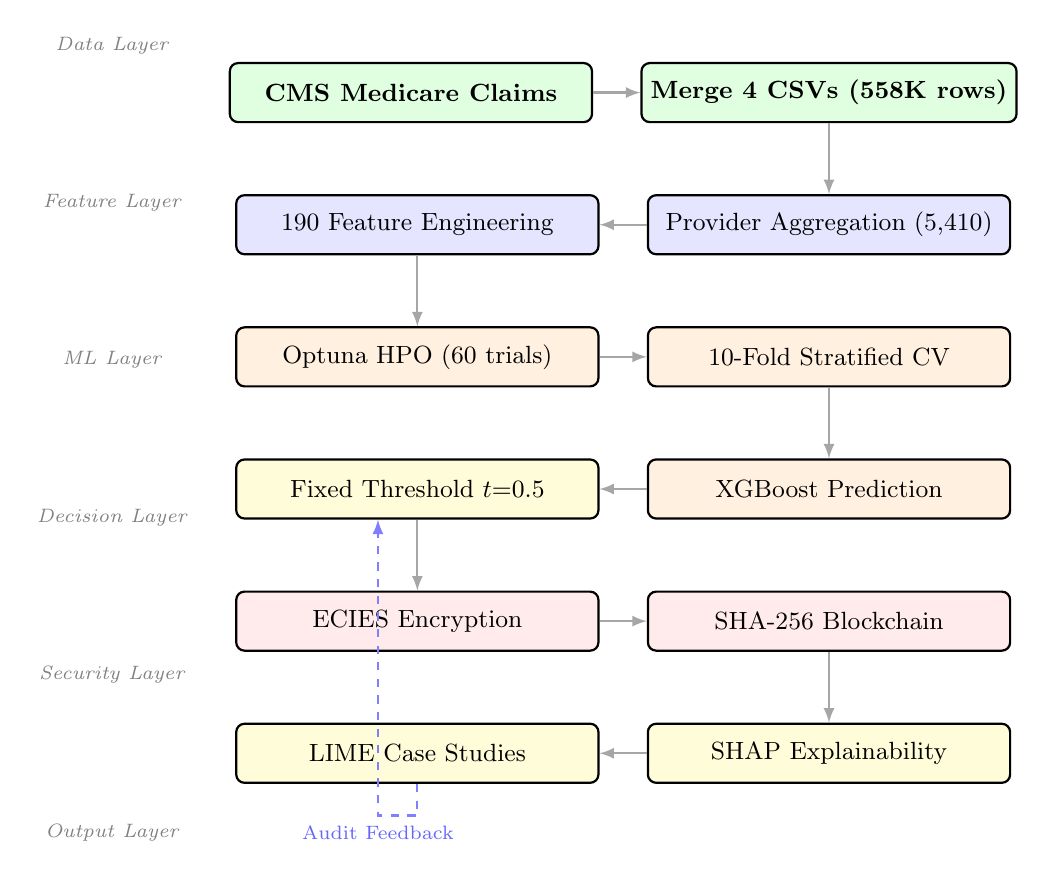
\begin{tikzpicture}[
    node distance=0.9cm and 0.6cm,
    data/.style={draw, rounded corners=3pt, fill=green!12, minimum width=4.6cm,
                 minimum height=0.75cm, align=center, font=\small\bfseries, thick},
    proc/.style={draw, rounded corners=3pt, fill=blue!10, minimum width=4.6cm,
                 minimum height=0.75cm, align=center, font=\small, thick},
    ml/.style={draw, rounded corners=3pt, fill=orange!12, minimum width=4.6cm,
               minimum height=0.75cm, align=center, font=\small, thick},
    sec/.style={draw, rounded corners=3pt, fill=red!8, minimum width=4.6cm,
                minimum height=0.75cm, align=center, font=\small, thick},
    outp/.style={draw, rounded corners=3pt, fill=yellow!15, minimum width=4.6cm,
                minimum height=0.75cm, align=center, font=\small, thick},
    arrow/.style={-latex, thick, color=gray!70},
    layer/.style={font=\scriptsize\itshape, text=gray}
]
% Row 1 (left to right): Data Layer
\node[layer] at (-3.8, 0.6) {Data Layer};
\node[data] (raw) at (0, 0) {CMS Medicare Claims};
\node[data, right=of raw] (merge) {Merge 4 CSVs (558K rows)};

% Row 2 (right to left): Feature Layer
\node[layer] at (-3.8, -1.4) {Feature Layer};
\node[proc, below=of merge] (agg) {Provider Aggregation (5,410)};
\node[proc, left=of agg] (feat) {190 Feature Engineering};

% Row 3 (left to right): ML Layer
\node[layer] at (-3.8, -3.4) {ML Layer};
\node[ml, below=of feat] (optuna) {Optuna HPO (60 trials)};
\node[ml, right=of optuna] (train) {10-Fold Stratified CV};

% Row 4 (right to left): Decision Layer
\node[layer] at (-3.8, -5.4) {Decision Layer};
\node[ml, below=of train] (pred) {XGBoost Prediction};
\node[outp, left=of pred] (thresh) {Fixed Threshold $t{=}0.5$};

% Row 5 (left to right): Security + Explainability Layer
\node[layer] at (-3.8, -7.4) {Security Layer};
\node[sec, below=of thresh] (ecies) {ECIES Encryption};
\node[sec, right=of ecies] (chain) {SHA-256 Blockchain};

% Row 6 (right to left): Output Layer
\node[layer] at (-3.8, -9.4) {Output Layer};
\node[outp, below=of chain] (shap) {SHAP Explainability};
\node[outp, left=of shap] (lime) {LIME Case Studies};

% Arrows: snake pattern
\draw[arrow] (raw) -- (merge);
\draw[arrow] (merge) -- (agg);
\draw[arrow] (agg) -- (feat);
\draw[arrow] (feat) -- (optuna);
\draw[arrow] (optuna) -- (train);
\draw[arrow] (train) -- (pred);
\draw[arrow] (pred) -- (thresh);
\draw[arrow] (thresh) -- (ecies);
\draw[arrow] (ecies) -- (chain);
\draw[arrow] (chain) -- (shap);
\draw[arrow] (shap) -- (lime);

% Feedback arrow from SHAP back to threshold
\draw[arrow, dashed, color=blue!50] (lime.south) -- ++(0,-0.4) -| ([xshift=-0.5cm]thresh.south) node[midway, below, font=\scriptsize, text=blue!60] {Audit Feedback};

\end{tikzpicture}
\caption{High-level architecture of the proposed ML and blockchain-based healthcare fraud detection pipeline. The snake layout illustrates the sequential data flow through six functional layers: data ingestion, feature engineering, model training, decision making, cryptographic security, and explainability output.}
\label{fig:ml_blockchain_arch}
\end{figure}

% ====================================================================
\section{Innovative Healthcare Insurance Fraud Detection}
% ====================================================================

The field of healthcare insurance fraud detection has undergone a significant methodological evolution over the past two decades, progressing from simple rule-based filters and manual audit sampling toward sophisticated data-driven systems that employ statistical learning, graph analysis, and distributed ledger technologies. Early detection systems were characterised by their reliance on fixed heuristics derived from known fraud patterns, which made them straightforwardly circumventable by fraudsters who adapted their schemes to avoid triggering pre-defined rules. The emergence of large-scale administrative claims databases - particularly the publicly available Centers for Medicare and Medicaid Services (CMS) datasets - has enabled the development and rigorous empirical evaluation of ML-based detection approaches at a scale and with a degree of reproducibility that was previously impossible \cite{ahmadian2020}. Modern approaches increasingly combine multiple complementary detection modalities, integrating supervised classification for provider-level fraud scoring, unsupervised anomaly detection for identifying novel fraud typologies, network analysis for uncovering collusion among providers, and blockchain-based audit trails for ensuring the integrity and non-repudiation of detection outcomes \cite{hassan2019}.

The present research contributes to this body of work by proposing and empirically validating a rigorous, reproducible pipeline for provider-level fraud detection that emphasises proper evaluation methodology, stratified cross-validation, and a systematic investigation of whether synthetic oversampling genuinely improves performance on imbalanced healthcare fraud datasets. The specific research objectives motivating this work are as follows:

\begin{enumerate}[label=\roman*.]
    \item To design and implement a rigorous feature engineering and normalisation pipeline for the CMS Medicare Part B provider-level fraud detection dataset, ensuring that all preprocessing steps respect the train-test boundary.
    \item To apply Bayesian hyperparameter optimisation using Optuna across five candidate machine learning classifiers - XGBoost, LightGBM, Gradient Boosting, CatBoost, and Random Forest - with stratified cross-validation to identify the best-performing configuration.
    \item To conduct a systematic ablation study on the effect of SMOTE-ENN synthetic oversampling on model performance under proper evaluation conditions, and to challenge the prevailing assumption that oversampling is universally beneficial for imbalanced fraud datasets.
    \item To integrate a SHA-256 blockchain with ECIES-encrypted patient data and smart contract-triggered investigative workflows into the fraud detection pipeline, thereby ensuring tamper-evidence, auditability, and privacy compliance.
    \item To provide comprehensive post-hoc model explainability through SHAP and LIME analyses, enabling human auditors to understand, validate, and trust the individual fraud classification decisions produced by the model.
\end{enumerate}

% ====================================================================
\section{Fraud Detection Issues and Challenges}
% ====================================================================

Healthcare fraud detection is a technically demanding problem that sits at the intersection of data science, information security, regulatory compliance, and clinical domain expertise. While machine learning and blockchain technologies offer powerful new tools for addressing fraud, their effective deployment in real-world healthcare systems requires navigating a complex landscape of interrelated challenges. This section provides a structured overview of the principal issues that practitioners must contend with when designing and deploying fraud detection systems for health insurance applications \cite{cruz2017,liang2019}.

% -------------------------------------------------------
\subsection{Sophisticated Fraud Schemes}
% -------------------------------------------------------

Modern healthcare fraud perpetrators employ increasingly sophisticated techniques designed specifically to evade detection by both human auditors and automated systems. Organised fraud networks coordinate the activities of multiple providers, clinics, and patient recruiters to generate large volumes of claims that are individually plausible but collectively fraudulent \cite{choi2020}. Collusive fraud schemes are particularly challenging because the consistency of documentation across multiple independent data sources makes them appear legitimate under standard single-entity audit procedures. As detection algorithms improve and are deployed at scale, fraudsters adapt their methods through a process akin to adversarial learning - subtly modifying billing patterns, rotating provider identities, and introducing noise to remain below algorithmic detection thresholds. This adversarial dynamic necessitates continuous model retraining and evaluation against evolving fraud distributions rather than treating detection as a one-time model deployment exercise.

% -------------------------------------------------------
\subsection{Data Volume and Variety}
% -------------------------------------------------------

National healthcare systems process hundreds of millions of insurance claims annually, generating datasets of substantial size and complexity. The CMS Medicare system alone adjudicates over one billion claims per year across Part A (inpatient), Part B (outpatient and physician), and Part D (prescription drug) programs. Effective fraud detection at this scale requires systems capable of processing high-velocity data streams in near real time, often within the latency constraints of automated adjudication workflows \cite{kumar2020}. Beyond sheer volume, healthcare claims data exhibits significant structural variety - incorporating diagnostic codes from the International Classification of Diseases (ICD), procedure codes from the Current Procedural Terminology (CPT), revenue codes, provider taxonomy codes, National Drug Codes (NDC), and demographic information - each governed by its own coding standards, versioning histories, and domain-specific semantics that must be correctly interpreted to extract meaningful fraud signals.

% -------------------------------------------------------
\subsection{Data Quality}
% -------------------------------------------------------

The effectiveness of any data-driven fraud detection system is fundamentally bounded by the quality of the underlying data. Healthcare administrative data is subject to a range of quality issues including missing values arising from optional fields in claim submission standards, systematic coding errors introduced by medical billing software, inconsistent use of modifier codes across providers and regions, and duplicate claim submissions arising from billing system errors rather than intentional fraud \cite{singh2021}. The presence of these data quality issues means that a significant pre-processing investment is required before any ML model can be reliably trained. Imputation strategies for missing values must be carefully chosen to avoid introducing bias into the feature space; for example, mean imputation for skewed reimbursement amounts can systematically underestimate the true degree of provider billing variability that is itself a fraud signal. The pipeline described in this work devotes substantial attention to reproducible pre-processing as a foundational requirement for valid model evaluation.

% -------------------------------------------------------
\subsection{Connecting to Outdated Computer Systems}
% -------------------------------------------------------

A significant practical barrier to the deployment of advanced fraud detection systems in healthcare is the prevalence of legacy information technology infrastructure across hospitals, insurers, and government health agencies. Many organisations continue to operate claims processing systems built on decades-old mainframe architectures or early-generation relational database management systems that predate modern data science tooling \cite{buczak2016}. Integrating ML-based detection modules with these legacy systems requires the development of bespoke data extraction, transformation, and loading (ETL) pipelines that can bridge incompatible data formats, authentication protocols, and network architectures. In many cases, real-time data feeds are not technically feasible, limiting fraud detection to retrospective batch analysis that introduces a lag between the time a fraudulent claim is submitted and the time it is flagged - during which additional fraudulent claims from the same actor may be processed and paid.

% -------------------------------------------------------
\subsection{Privacy Concerns}
% -------------------------------------------------------

Healthcare data is among the most sensitive categories of personal information, subject to strict regulatory protection under frameworks including the Health Insurance Portability and Accountability Act (HIPAA) in the United States, the General Data Protection Regulation (GDPR) in the European Union, and equivalent national legislation in jurisdictions worldwide \cite{he2019}. Fraud detection systems necessarily require access to detailed claims data that contains or can be linked to individually identifiable patient information. Balancing the need for analytical access to support fraud detection against the legal and ethical obligations to protect patient privacy requires careful system design. Techniques such as data anonymisation, differential privacy, federated learning, and field-level encryption - as employed through ECIES in this work - provide partial solutions, but each introduces trade-offs in detection accuracy, computational cost, or operational complexity that must be explicitly managed.

% -------------------------------------------------------
\subsection{Lack of Standardization}
% -------------------------------------------------------

Healthcare data standards vary considerably across countries, health systems, insurance products, and time periods. Diagnostic coding systems have transitioned from ICD-9 to ICD-10 and are moving toward ICD-11, while procedure coding varies between CPT, HCPCS, and national equivalents. These transitions create temporal discontinuities in claims databases that can mislead models trained on historical data when applied to current claims \cite{eling2018}. Beyond coding standards, the lack of a universal provider identifier, inconsistent definitions of claim fields across payer systems, and heterogeneous data exchange formats all impede the development of fraud detection models that can be readily generalised from one health system or insurance market to another. This fragmentation of standards also complicates the creation of cross-institutional datasets large enough to support robust training of deep learning models.

% -------------------------------------------------------
\subsection{Security of HI System}
% -------------------------------------------------------

The healthcare insurance system is not only vulnerable to fraud from external actors but also faces internal security threats from employees who have privileged access to claims data and adjudication systems \cite{elemam2013}. Insider threats may involve the deliberate manipulation of claims outcomes, the disclosure of patient data to external fraud networks, or the sabotage of fraud detection workflows. Beyond insider threats, healthcare information systems are high-value targets for external cyberattacks including ransomware campaigns that encrypt claims databases and demand payment for their restoration. A robust fraud detection infrastructure must therefore incorporate information security controls - including role-based access control, multi-factor authentication, encrypted data-at-rest and data-in-transit, and continuous security monitoring - that protect both the integrity of fraud detection outcomes and the confidentiality of the patient data on which they are based.

% -------------------------------------------------------
\subsection{Resource Constraints}
% -------------------------------------------------------

Effective fraud detection requires sustained investment in computational infrastructure, data science expertise, and operational processes for investigating and acting on flagged claims \cite{yoo2015}. Many health insurance organisations - particularly smaller regional insurers and government health programs in lower-income countries - lack the financial and human capital resources to develop and maintain sophisticated ML-based detection systems. Open-source tools and cloud-based computing services have substantially reduced the barrier to entry for deploying ML models, but the operational costs of model maintenance, re-training, and continuous evaluation remain non-trivial. The Special Investigation Unit (SIU) investigators who must follow up on algorithmically flagged claims represent a fixed investigative capacity that can easily be overwhelmed if detection systems generate large volumes of false positives, creating a practical ceiling on the effective sensitivity of deployed fraud detection systems.

% -------------------------------------------------------
\subsection{Cross-Channel Fraud}
% -------------------------------------------------------

Modern healthcare fraud increasingly operates across multiple channels and claim types simultaneously, exploiting inconsistencies between the oversight mechanisms applied to different segments of the healthcare system \cite{kumar2011}. A single fraud scheme may involve fabricated inpatient claims submitted under Part A, inflated physician billing under Part B, and fraudulent prescription drug claims under Part D - with each component appearing normal when examined in isolation within its own program but revealing a coordinated pattern only when data across programs is integrated and analysed jointly. Cross-channel fraud detection therefore requires not only within-channel anomaly detection but also the capacity to link identities and activities across disparate data sources, which is technically challenging when provider and patient identifiers are not consistently maintained across systems.

% -------------------------------------------------------
\subsection{Regulatory Challenges}
% -------------------------------------------------------

Healthcare fraud detection systems operate within a complex and evolving regulatory environment that constrains both the data that may be used for detection and the actions that may be taken in response to flagged claims \cite{dutt2020}. Regulations governing data retention, patient consent, algorithmic decision-making, and anti-discrimination must all be observed when designing and deploying automated detection systems. Increasingly, regulatory frameworks are demanding explainability for automated decisions that affect individuals - including the denial or investigation of insurance claims - which places additional requirements on the interpretability of detection models beyond what would be required purely on accuracy grounds. In the European Union, the AI Act introduces specific obligations for AI systems used in high-risk contexts such as healthcare, requiring conformity assessments, transparency disclosures, and human oversight provisions that must be built into the detection pipeline from the outset.

% -------------------------------------------------------
\subsection{Machine Learning and AI Limitations}
% -------------------------------------------------------

While ML techniques have demonstrated strong empirical performance on historical fraud detection benchmarks, they carry inherent limitations that are particularly consequential in the healthcare domain \cite{gerke2019}. Class imbalance is a fundamental challenge: in most healthcare claims datasets, fraudulent claims constitute a small minority of total records, creating a statistical environment in which a classifier that labels all claims as legitimate can achieve deceptively high accuracy. Standard performance metrics such as overall accuracy therefore fail to capture the practically relevant capability of the model to correctly identify the fraudulent minority. The pipeline in this work uses AUC-PR (Area Under the Precision-Recall Curve) as the primary optimisation objective, a choice that directly addresses this imbalance by emphasising performance on the positive (fraud) class. ML models are also susceptible to distribution shift - their performance degrades when the statistical characteristics of current claims data diverge from those of the training set - necessitating regular re-evaluation and re-training against updated data.

% -------------------------------------------------------
\subsection{Human Expertise}
% -------------------------------------------------------

Despite the potential of automated systems to process data at a scale and speed beyond human capacity, healthcare fraud detection ultimately requires deep collaboration between algorithmic systems and experienced human investigators \cite{abdallah2016}. Clinical domain expertise is indispensable for interpreting the significance of specific billing patterns, understanding the legitimate clinical rationale for unusual treatment sequences, and exercising judgment in ambiguous cases where algorithmic scores alone are insufficient to determine fraud. Experienced investigators also play a critical role in providing labelled data through confirmed fraud cases, feeding the supervised learning pipeline that underpins model training. The scarcity of this expertise - combined with high investigator turnover, institutional knowledge loss, and the cognitive burden of reviewing large volumes of algorithmically flagged cases - represents a persistent bottleneck in the operationalisation of fraud detection systems, regardless of their algorithmic sophistication.

% ====================================================================
\section{Taxonomy of Health Insurance Fraud Detection}
% ====================================================================

The academic and applied literature on health insurance fraud detection encompasses a rich diversity of methodological approaches, each with distinct strengths, limitations, and areas of applicability. Structuring this diversity into a coherent taxonomy facilitates comparative evaluation and helps practitioners select the most appropriate detection strategy for a given operational context. The principal methodological families are reviewed in the following subsections, drawing on a representative selection of landmark studies to illustrate the capabilities and limitations of each approach \cite{pareek2023,hilal2022}.

% -------------------------------------------------------
\subsection{Supervised Learning}
% -------------------------------------------------------

Supervised learning approaches train classification models using labelled historical data in which individual claims or providers have been identified as either fraudulent or legitimate by human investigators or regulatory authorities \cite{duman2017}. A wide range of supervised algorithms has been applied to HI fraud detection, including logistic regression, decision trees, random forests, gradient-boosted machines, support vector machines, and deep neural networks. The primary strength of supervised approaches is their capacity to learn highly non-linear discriminative boundaries in high-dimensional feature spaces, enabling them to detect complex fraud patterns that would be invisible to rule-based systems. The principal limitation is their dependence on large quantities of accurately labelled training data, which is expensive and time-consuming to produce and is frequently subject to label noise arising from cases where fraud was suspected but not definitively proven. Class imbalance is an additional structural challenge, as fraudulent claims typically represent a small fraction of total claims volume, and standard training objectives can cause models to over-fit to the majority class at the expense of fraud detection sensitivity \cite{kose2015}.

% -------------------------------------------------------
\subsection{Unsupervised Learning}
% -------------------------------------------------------

Unsupervised learning methods detect fraud by identifying claims or providers whose statistical characteristics deviate significantly from the norm without requiring prior labelled examples of fraud \cite{zhou2020}. Clustering algorithms such as k-means, DBSCAN, and Gaussian mixture models partition the claims population into groups of similar entities and flag members of small or outlying clusters as anomalous. Autoencoders and other deep generative models learn a compact latent representation of normal claims data and detect fraud through elevated reconstruction error on claims that do not conform to learned normal patterns. The principal advantage of unsupervised approaches is their ability to detect novel fraud typologies that have not been previously observed and thus cannot be captured by supervised models trained on historical fraud labels. Their limitation is the absence of a direct optimisation objective tied to fraud detection, which can result in high false-positive rates as legitimate but unusual claims are flagged alongside genuinely fraudulent ones \cite{tsai2019}.

% -------------------------------------------------------
\subsection{Hybrid Approach}
% -------------------------------------------------------

Hybrid approaches combine supervised and unsupervised techniques to capitalise on the complementary strengths of each paradigm. A common architecture uses an unsupervised anomaly detector as a first-stage filter to identify suspicious claims warranting closer examination, followed by a supervised classifier trained on confirmed fraud labels to make a final determination on the pre-filtered set \cite{wang2021deep}. Alternatively, unsupervised clustering can be used to generate pseudo-labels for unlabelled data, which are then used to augment a supervised training set in a semi-supervised learning framework. Hybrid approaches have demonstrated improvements in both precision and recall relative to either pure supervised or pure unsupervised baselines in multiple published evaluations, and they offer a practical pathway for deploying effective fraud detection in settings where labelled data is scarce \cite{ahmadian2020}. The ensemble architecture adopted in this work - combining Optuna-tuned XGBoost, LightGBM, CatBoost, and other classifiers through a voting scheme - represents a form of supervised ensemble hybridisation that benefits from diversity among base learners.

% -------------------------------------------------------
\subsection{HIC Fraud Detection from Group of People}
% -------------------------------------------------------

Group-level fraud detection recognises that healthcare fraud is frequently a collective rather than an individual phenomenon, involving coordinated activity among networks of providers, patients, and administrative staff \cite{sun2018patient}. Graph-theoretic and social network analysis methods model the relationships among healthcare entities as a network, with nodes representing providers or patients and edges representing referral relationships, shared billing patterns, or co-occurring diagnoses. Community detection algorithms identify dense subgraphs that may represent collusive fraud rings, while anomalous edge weights or unusual community membership patterns serve as fraud indicators. This approach is particularly effective for detecting the organised fraud schemes that account for a disproportionate share of total fraud losses, as the network structure of these schemes leaves a distinctive statistical signature even when individual transactions appear legitimate in isolation \cite{hassan2019}.

% -------------------------------------------------------
\subsection{Blockchain-Based HIC Fraud Prevention}
% -------------------------------------------------------

Blockchain technology provides a fundamentally different approach to fraud prevention - one focused on making fraud more difficult to perpetrate rather than on detecting it after the fact. By recording claims data, adjudication decisions, and payment transactions on a distributed, immutable ledger, blockchain creates a transparent and tamper-evident audit trail that exposes the data manipulation and identity falsification on which many fraud schemes depend \cite{alhashedi2021}. Smart contracts can enforce claims adjudication rules automatically and consistently, eliminating the discretionary decision-making that is sometimes exploited in manual approval workflows. The cryptographic properties of blockchain - including digital signatures for provider identity verification and hash-based integrity checking for claims data - provide strong authenticity guarantees that are technically very difficult to circumvent. Practical implementations must address challenges of scalability, latency, and interoperability with existing healthcare IT infrastructure, but proof-of-concept systems have demonstrated the viability of blockchain-based fraud prevention in pilot deployments \cite{amponsah2022}.

% -------------------------------------------------------
\subsection{AI and Blockchain-Based HIC Fraud Detection}
% -------------------------------------------------------

The integration of AI and blockchain technologies represents the most comprehensive approach to HI fraud detection currently available, combining the predictive power of machine learning with the auditability and integrity guarantees of distributed ledger technology \cite{li2021}. In such integrated architectures, ML models process claims data in real time to generate fraud probability scores, which are then recorded on the blockchain alongside the encrypted features used to produce them. This creates a verifiable, non-repudiable record of every fraud assessment decision that can be audited by regulators, insurers, and - where appropriate under data protection law - patients themselves. Smart contracts can automate the downstream workflow triggered by high fraud scores, initiating investigative queues, placing payment holds, or notifying relevant oversight authorities without requiring manual intervention \cite{pareek2023}. The SHAP-based explainability layer included in the present work addresses the additional requirement that AI-generated fraud assessments be interpretable by human reviewers, bridging the gap between algorithmic sophistication and operational accountability.

% ====================================================================
\section{Security and Privacy Requirements of Healthcare Applications}
% ====================================================================

Healthcare applications that process, store, or transmit patient and claims data must satisfy a comprehensive set of security and privacy requirements derived from both regulatory mandates and fundamental information security principles. Failure to meet any of these requirements creates vulnerabilities that can be exploited both by fraudsters seeking to manipulate the claims process and by malicious actors seeking to obtain sensitive patient data for identity theft, blackmail, or other harmful purposes. The following subsections describe the principal security and privacy requirements applicable to health insurance fraud detection systems, with reference to their specific relevance in the context of the proposed ML and blockchain-based pipeline \cite{zeadally2020,alomar2021}.

% -------------------------------------------------------
\subsection{Data Confidentiality}
% -------------------------------------------------------

Data confidentiality ensures that sensitive healthcare information is accessible only to those parties with an explicit, authorised need to access it - and is shielded from all other parties including potential eavesdroppers on communication networks and unauthorised internal users \cite{elemam2013}. In the context of health insurance fraud detection, confidentiality applies to patient demographics, diagnosis and procedure codes, provider identities, and reimbursement amounts - all of which are sensitive either individually or in combination. The Elliptic Curve Integrated Encryption Scheme (ECIES) employed in the blockchain component of this work provides strong asymmetric encryption of patient-identifiable data fields before they are committed to the ledger, ensuring that only authorised investigators holding the corresponding private key can decrypt and view individual patient records while the fraud assessment scores remain transparent to auditors.

% -------------------------------------------------------
\subsection{Data Authentication}
% -------------------------------------------------------

Data authentication mechanisms ensure that the provenance of healthcare records can be verified - that a claim, diagnosis code, or treatment record was genuinely submitted by the party that purports to have submitted it, and that it has not been modified in transit or at rest \cite{hassan2019}. In the blockchain component of the proposed system, each block is identified by a SHA-256 cryptographic hash that incorporates the hash of the preceding block, creating a chain structure in which any modification to a historical record immediately invalidates all subsequent hashes and is thus instantly detectable. Digital signatures applied at the point of claim submission further ensure that records can be traced to their originating provider entity, providing non-repudiation guarantees that are essential for supporting legal proceedings against identified fraudsters.

% -------------------------------------------------------
\subsection{Strong User Authentication}
% -------------------------------------------------------

Access to fraud detection systems and the sensitive data they process must be protected by robust user authentication mechanisms that prevent unauthorised individuals from querying fraud scores, accessing patient records, or manipulating detection parameters \cite{yoo2015}. Multi-factor authentication, combining something the user knows (a password), something the user has (a hardware token or mobile device), and optionally something the user is (a biometric factor), provides substantially stronger access control than single-factor password-based authentication, which is vulnerable to credential theft and brute-force attacks. Role-based access control ensures that different categories of system users - data scientists, claims investigators, compliance officers, and patients - have access only to the specific system functions and data fields relevant to their role, implementing the principle of least privilege as a foundational security control.

% -------------------------------------------------------
\subsection{Data Integrity}
% -------------------------------------------------------

Data integrity requirements mandate that healthcare records must remain accurate, complete, and unmodified from the time of creation through the entire lifecycle of their storage and processing \cite{abdallah2016}. Any unauthorised modification to a claims record - whether by an external attacker, a malicious insider, or a software bug - must be detectable. In the proposed system, the SHA-256 Merkle tree structure of the blockchain provides cryptographic integrity guarantees for all committed records. Additionally, the feature engineering pipeline applies reproducible, deterministic transformations with explicit version control to ensure that the feature vectors committed to the blockchain can be independently verified against the raw claims data from which they were derived. Data integrity in the ML training pipeline is equally critical: contamination of the training set with mislabelled records or improperly handled missing values can systematically bias learned model parameters in ways that are difficult to detect post-hoc.

% -------------------------------------------------------
\subsection{Key Distribution}
% -------------------------------------------------------

The security of any cryptographic system ultimately depends on the secure generation, storage, distribution, and revocation of the cryptographic keys used to enforce confidentiality and authentication \cite{ahmadian2020}. In the ECIES implementation employed in this work, public-private key pairs are generated for each authorised system participant. Public keys are distributed through a trusted key registry and are used by data submitters to encrypt patient data fields before blockchain commitment. Private keys are held exclusively by authorised investigators and must be stored in hardware security modules or equivalent tamper-resistant environments to prevent extraction. Key revocation procedures must be in place to immediately withdraw access when an investigator leaves the organisation, when a key is suspected to have been compromised, or when access privileges change as a result of a role change, ensuring that former employees or compromised credentials cannot be used to access historical fraud investigation records.

% -------------------------------------------------------
\subsection{Access Control}
% -------------------------------------------------------

Comprehensive access control mechanisms govern which system components, data fields, and operational capabilities each category of user or automated process can interact with \cite{gerke2019}. In the fraud detection pipeline, access control operates at multiple levels: at the data layer, determining which raw claims fields can be queried; at the model layer, determining who can inspect model parameters, re-train classifiers, or adjust detection thresholds; and at the blockchain layer, determining which entities can submit new transactions, query fraud assessment records, or invoke smart contract functions. Attribute-based access control (ABAC) policies that incorporate contextual factors such as the user's organisational role, the sensitivity classification of the requested data, the purpose of the access request, and the current regulatory compliance status of the requesting entity provide a flexible and fine-grained framework for enforcing appropriate access restrictions across the diverse set of stakeholders involved in a healthcare fraud detection ecosystem.

% -------------------------------------------------------
\subsection{Data Availability}
% -------------------------------------------------------

Data availability requirements ensure that fraud detection systems and the healthcare data they depend on remain accessible and operational when needed, even in the face of hardware failures, software errors, network disruptions, or deliberate denial-of-service attacks \cite{zeadally2020}. Availability is particularly critical in fraud detection contexts where system downtime can result in the unvetted processing of fraudulent claims. The distributed architecture of blockchain systems provides inherent availability benefits through replication: the ledger is maintained across multiple independent nodes, ensuring that no single point of failure can render historical fraud records inaccessible. For the ML inference components, high availability is typically achieved through redundant model serving infrastructure with load balancing and automatic failover, combined with graceful degradation policies that allow claims to be processed under enhanced manual scrutiny when automated scoring is temporarily unavailable.

% -------------------------------------------------------
\subsection{Data Freshness}
% -------------------------------------------------------

Data freshness requirements address the need to ensure that the information on which fraud detection decisions are based is current and has not been replaced by outdated or replayed data \cite{tian2019}. In distributed healthcare systems, an attacker who can replay old claims or substitute stale data records for current ones may be able to circumvent fraud detection by replacing suspicious recent transactions with historical legitimate ones. Cryptographic timestamps embedded in each blockchain block, combined with sequence number enforcement in the claims processing pipeline, provide strong guarantees that each transaction processed by the fraud detection system is genuinely new and has not been previously seen or replayed from an earlier point in time. Freshness of the ML model itself is equally important: a model trained on data from several years ago may fail to detect current fraud schemes that did not exist at the time of training, necessitating regular re-training and evaluation against recent labelled data.

% -------------------------------------------------------
\subsection{Secure Localization}
% -------------------------------------------------------

Secure localisation in healthcare systems refers to the ability to reliably and tamper-resistantly associate a data record or transaction with its physical or logical point of origin \cite{mohanty2016}. In the context of health insurance claims, this encompasses the accurate identification of the provider location where a service was allegedly rendered - a key variable in detecting geographically implausible claims, such as a patient supposedly receiving services at facilities hundreds of miles apart on the same day. Secure localisation also applies to the integrity of provider directory information, ensuring that the facility addresses and geographic service areas associated with provider identifiers in the claims system are genuine and have not been falsified to support phantom billing schemes. Integration of geolocation data into the feature engineering pipeline can yield powerful fraud signals when cross-validated against patient home addresses and provider catchment areas.

% -------------------------------------------------------
\subsection{Patient Permission}
% -------------------------------------------------------

Respect for patient autonomy requires that individuals whose data is used in fraud detection systems have meaningful control over how their health information is accessed, processed, and shared \cite{gerke2019,pareek2023}. Informed consent frameworks must clearly communicate to patients that their claims data may be used for fraud detection purposes, what safeguards are in place to protect their privacy, who has access to fraud assessment records derived from their data, and what recourse they have if they believe their data has been mishandled or if they have been incorrectly flagged. The growing adoption of patient-centred data governance models - in which individuals can grant and revoke access permissions for their records through digital consent management platforms - aligns naturally with blockchain-based systems where access control policies can be encoded as smart contracts and their enforcement made auditable and transparent to patients in real time. Ensuring patient permission is not merely an ethical obligation but an increasingly explicit legal requirement under data protection frameworks in jurisdictions worldwide.

\chapter{Literature Review}

\section{Overview}

Healthcare insurance fraud represents one of the most persistent and financially devastating challenges facing modern healthcare systems worldwide. The National Health Care Anti-Fraud Association estimates that fraudulent billing, upcoding, and phantom services collectively drain billions of dollars annually from public and private health insurance programmes, with losses in the United States alone accounting for approximately 3 to 10 percent of total healthcare expenditure \cite{nhcaa2021}. These losses are not merely financial; they divert resources from legitimate patient care, inflate premiums, and erode public trust in healthcare institutions. The problem is compounded by the sheer scale and complexity of healthcare billing ecosystems, where millions of claims are processed daily across thousands of providers, making manual auditing both impractical and insufficient as a primary control mechanism.

The convergence of machine learning and blockchain technology has emerged as a particularly promising strategy to address the limitations of conventional fraud detection systems. Traditional rule-based systems, while deterministic and interpretable, are inherently reactive and struggle to adapt to evolving fraudulent patterns. Machine learning methods offer the capacity to detect subtle, multi-dimensional anomalies in claim data that would elude manual review, while blockchain architectures provide tamper-evident audit trails and decentralised consensus mechanisms that reduce opportunities for data manipulation and collusion \cite{amponsah2022}. Recent research has demonstrated that hybrid frameworks combining predictive modelling with distributed ledger technology can substantially improve detection accuracy while simultaneously providing verifiable provenance for audit decisions \cite{li2021}. This combination addresses both the detection and the accountability dimensions of the fraud problem.

This chapter reviews twenty-two studies drawn from the peer-reviewed literature spanning 2016 to 2024, covering a range of machine learning techniques, sampling strategies, blockchain integration approaches, and model explainability methods relevant to healthcare insurance fraud detection. The review is structured as a narrative synthesis of individual contributions, followed by a comparative summary table and a discussion of the gaps in existing literature that the present study addresses. The reviewed works collectively represent the state of the art in algorithmic fraud detection, from classical ensemble methods and deep learning architectures to attention-based graph networks and smart contract implementations.

\section{Review of Individual Studies}

Mohammed et al.\ \cite{mohammed2023} conducted a comparative evaluation of six supervised machine learning algorithms applied to a blockchain-based healthcare fraud detection framework. The algorithms examined were Logistic Regression, Decision Tree, K-Nearest Neighbours, Naive Bayes, Support Vector Machine, and Random Forest, each evaluated on a labelled healthcare claims dataset integrated with a simulated blockchain environment. The study measured accuracy, precision, recall, F1-score, and execution time across all models. Random Forest achieved the highest overall accuracy and demonstrated the most favourable trade-off between detection performance and computational runtime, outperforming single estimator models by a significant margin. The authors concluded that ensemble methods are particularly well-suited to the class-imbalanced, high-dimensional characteristics of healthcare claims data, and that embedding the fraud classification pipeline within a blockchain layer adds a meaningful layer of provenance without substantially degrading throughput.

Lopo et al.\ \cite{lopo2023} investigated the effect of class imbalance mitigation strategies on XGBoost-based healthcare fraud detection, comparing the Synthetic Minority Oversampling Technique (SMOTE) with Instance Hardness Threshold (IHT) undersampling at multiple class distribution ratios. The authors experimented with majority-to-minority distribution splits ranging from 50-50 to 90-10, evaluating each configuration on standard classification metrics. Their results showed that a 70 percent majority to 30 percent minority distribution, combined with SMOTE oversampling applied to the minority fraud class, produced the optimal balance between recall and precision for the XGBoost classifier. IHT-based undersampling consistently produced lower recall values, indicating a tendency to discard informative borderline instances. The study highlighted that the choice of resampling ratio is a critical but often overlooked hyperparameter in fraud detection pipelines.

Johnson et al.\ \cite{johnson2023} addressed a methodologically significant problem in healthcare fraud detection evaluation: the risk of evaluation target leakage introduced by standard cross-validation procedures when applied to provider-level fraud datasets. The authors demonstrated that naive k-fold cross-validation, when applied without grouping by provider, allows information from a single provider's claims to appear in both training and test folds, artificially inflating reported performance metrics. They proposed a modified grouped cross-validation scheme applied to Medicare claims data, ensuring that all claims from a given provider are assigned exclusively to either the training or the evaluation partition. XGBoost and Random Forest were evaluated under both the naive and the corrected protocols, and the corrected procedure yielded substantially lower but more realistic performance estimates, underscoring the importance of evaluation rigour in this domain.

Lu et al.\ \cite{lu2023} proposed a multi-level heterogeneous attention network for medical fraud detection, referred to as MHAMFD, designed to operate on an attributed heterogeneous information network (AHIN) constructed from Medicare claims records. The framework encodes relationships among providers, patients, and diagnostic codes as a heterogeneous graph and applies multi-head attention mechanisms at both the node and the edge levels to learn discriminative fraud-relevant representations. Evaluated on a Medicare-derived benchmark, MHAMFD achieved an accuracy of 91.94 percent, outperforming baseline graph neural network models including GraphSAGE and GAT. The authors attributed the performance gains to the model's capacity to capture cross-type relational signals that homogeneous graph models cannot represent, establishing attention-based graph learning as a promising direction for large-scale fraud detection.

Nalluri et al.\ \cite{nalluri2023} conducted a systematic comparison of Support Vector Machine, Decision Tree, Random Forest, and Multilayer Perceptron classifiers on two distinct healthcare fraud datasets, evaluating performance under consistent preprocessing and feature engineering conditions. The experimental design controlled for data leakage, and both datasets underwent standard normalisation before model fitting. The Multilayer Perceptron achieved the highest accuracy of 95.29 percent across the combined evaluation, benefiting from its ability to learn non-linear feature interactions that linear and shallow tree-based models could not capture. Decision Tree produced the lowest performance, consistent with its susceptibility to overfitting on tabular medical claims data. The study reinforced the value of neural architectures even in relatively moderate-scale healthcare fraud settings.

Amponsah et al.\ \cite{amponsah2022} presented a hybrid fraud detection system that combined a Decision Tree classifier with an Ethereum blockchain-based smart contract infrastructure for healthcare claims management. The Decision Tree model was trained on a publicly available healthcare fraud dataset and achieved a classification accuracy of 97.96 percent, with the smart contract layer used to record, hash, and verify individual claim decisions on the Ethereum test network. The authors demonstrated that the on-chain verification component added a non-repudiable audit trail without materially increasing end-to-end processing latency. This work is among the earliest to couple a fully functional blockchain deployment with a quantitatively validated machine learning component, making it a foundational reference for blockchain-integrated fraud detection research.

Sathya and Balakumar \cite{sathya2022} proposed the Enhanced Random Forest and Support Vector Machine (eRFSVM) hybrid classifier, which combined the feature selection strengths of Random Forest with the margin-maximising decision boundary of SVM within a unified classification pipeline anchored to a blockchain audit framework. The model was evaluated on a medical insurance claims dataset, achieving an accuracy of 97.176 percent alongside precision and recall values that exceeded those of the constituent single models. The blockchain layer was implemented to ensure immutability of claim records and to provide a secure reference for the classifier's historical decisions. The eRFSVM framework demonstrated that carefully engineered hybrid classifiers can surpass both component models individually, and that blockchain integration can be made computationally practical at small to medium dataset scales.

Kumaraswamy et al.\ \cite{kumaraswamy2022} developed a prescription claim fraud detection framework targeting pharmacy billing irregularities, evaluating Logistic Regression, Decision Tree, Random Forest, and Gradient Boosting on a proprietary prescription claims dataset. Performance was measured using the area under the receiver operating characteristic curve (AUC-ROC), precision, recall, and F1-score. Logistic Regression achieved the highest AUC-ROC of 0.76, a result the authors attributed to the relatively linear separability of the prescription fraud signal in the feature space constructed from temporal prescribing patterns and dosage anomalies. The study also highlighted the difficulty of working with severely class-imbalanced prescription datasets and recommended threshold calibration as a post-training step to improve operational recall.

Gangadhar et al.\ \cite{gangadhar2022} introduced a Chaotic Variational Autoencoder (C-VAE) for unsupervised anomaly detection in health insurance claims, augmenting a standard variational autoencoder with a chaotic mapping function in the latent space to improve the diversity of synthetic anomaly reconstructions. The model was evaluated on a health insurance (HI) claims dataset and achieved an anomaly detection accuracy of 77.9 percent, with the chaotic perturbation demonstrably improving recall over a standard VAE baseline. The authors argued that generative anomaly detection approaches are preferable to purely supervised methods when labelled fraud examples are scarce, as the model learns the distribution of legitimate claims and flags deviations accordingly. The C-VAE represents an important contribution to the growing body of generative modelling approaches for healthcare fraud.

Aziz et al.\ \cite{aziz2022} applied the LightGBM (LGBM) gradient boosting framework to the detection of fraudulent activity on the Ethereum blockchain, constructing features from transaction graph statistics, gas usage patterns, and temporal behavioural signals extracted from on-chain data. The baseline LGBM model achieved an accuracy of 98.60 percent on the labelled Ethereum fraud dataset, and a subsequent fine-tuning phase using Bayesian hyperparameter optimisation raised accuracy to 99.03 percent. The study demonstrated that gradient boosting methods combined with thoughtfully engineered graph-based features can achieve near-ceiling performance on blockchain transaction fraud, and the fine-tuning gains underscored the value of systematic hyperparameter search even for already high-performing models.

Hancock and Khoshgoftaar \cite{hancock2021} performed a head-to-head comparison of CatBoost and LightGBM for Medicare fraud detection, using the Centers for Medicare and Medicaid Services (CMS) Provider Utilization and Payment Data as the primary dataset. Both models were evaluated under consistent preprocessing and class weighting conditions, with performance assessed via AUC-ROC, F1-score, and Matthews correlation coefficient. CatBoost achieved an AUC-ROC of 0.8824, marginally outperforming LightGBM, and demonstrated greater stability across multiple random seeds. The authors attributed CatBoost's advantage to its ordered boosting mechanism, which reduces prediction shift bias on categorical features prevalent in Medicare provider data. This study established CatBoost as a competitive baseline for Medicare fraud benchmarking.

Bhaskar et al.\ \cite{bhaskar2021} applied the Isolation Forest algorithm to healthcare insurance fraud detection in a fully unsupervised setting, exploiting the algorithm's ability to isolate anomalies by recursively partitioning the feature space with randomly selected split points and thresholds. The model was evaluated on a healthcare claims dataset and achieved an accuracy of 98.76 percent, a strong result for an unsupervised approach. The authors demonstrated that Isolation Forest is computationally efficient and scales well to high-dimensional claim records, making it suitable for real-time deployment scenarios where labelled fraud data may not be available at the time of scoring. This work highlighted the practical value of anomaly detection frameworks as complements to supervised classifiers in production fraud detection systems.

Dhieb et al.\ \cite{dhieb2020} proposed an extreme gradient boosting (XGBoost) based insurance fraud detection system integrated with a blockchain layer for secure data sharing and tamper-proof storage of model decisions. The XGBoost classifier outperformed a Decision Tree baseline by approximately 7 percentage points in accuracy, with additional gains in precision and recall attributable to XGBoost's regularisation mechanisms and iterative residual correction. The blockchain component was designed to facilitate multi-party claim processing, allowing insurers, providers, and auditors to share a verified view of claim status without exposing raw data to all parties. This combination of predictive accuracy and cryptographic data governance represented an early and influential model for the hybrid ML-blockchain paradigm in insurance fraud research.

Matloob et al.\ \cite{matloob2020} explored sequential pattern mining as an alternative to instance-level classification for detecting healthcare fraud, employing Prefix Span and Compact Prediction Tree (CPT) algorithms to identify suspicious temporal sequences of claim events within provider billing histories. The framework treated consecutive claim submissions as sequences and mined frequent fraudulent patterns that could not be detected by models operating on individual claim records in isolation. Across multiple experimental configurations, the approach achieved an average accuracy of 85 percent, with CPT demonstrating stronger pattern completion performance than Prefix Span. The study contributed an important methodological perspective, demonstrating that the temporal structure of billing behaviour carries substantial fraud signal that is systematically ignored by standard feature-based classifiers.

Gera et al.\ \cite{gera2020} designed an insurance claims management system built on the IBM Hyperledger Fabric permissioned blockchain, enabling peer-based claim settlement among insurance consortium members without requiring a central adjudicating authority. The system encoded claim validation and settlement logic as chaincode smart contracts, allowing claims to be reviewed, approved, and recorded on an immutable distributed ledger shared among all consortium participants. While the work did not incorporate a machine learning component, it provided a detailed technical blueprint for enterprise-grade blockchain deployment in insurance, including access control, identity management, and endorsement policy design. The IBM Hyperledger approach documented by Gera et al.\ remains the most practically detailed blockchain architecture in the healthcare fraud literature reviewed here.

Johnson et al.\ \cite{johnson2019} investigated deep learning approaches for Medicare fraud detection with a focus on the class imbalance problem, applying combined random oversampling and random undersampling (ROS-RUS) strategies to a Medicare beneficiary claims dataset. A feedforward neural network was trained under multiple imbalance correction conditions, and the ROS-RUS hybrid strategy achieved the best AUC-ROC of 0.8509 among the configurations tested. The authors found that purely oversampling-based approaches tended to overfit to replicated minority class instances, while purely undersampling approaches discarded substantial majority class information; the hybrid strategy balanced these competing risks most effectively. This study established a quantitative benchmark for deep learning-based Medicare fraud detection and highlighted the centrality of imbalance handling in neural classifier performance.

Bauder and Khoshgoftaar \cite{bauder2017} provided an early systematic analysis of gradient boosting methods applied to Medicare fraud detection at the provider level, constructing aggregate provider-level feature vectors from CMS claims data and training gradient boosting classifiers to identify fraudulent providers. The study evaluated multiple boosting configurations and established provider-level AUC-ROC baselines that subsequent Medicare fraud research has used as reference points. The authors emphasised the importance of feature engineering at the provider level, noting that aggregated billing behaviour features were far more informative than raw claim-level features for provider fraud classification. This work laid an important empirical foundation for subsequent studies in the Medicare fraud detection literature.

Sun et al.\ \cite{sun2018} proposed the Abnormal Group Joint Fraud Detection (AGJFD) framework, designed to detect collusive fraud rings among multiple healthcare providers who coordinate false billing across shared patient pools. The method modelled provider-patient relationships as a bipartite graph and applied joint inference across connected providers to amplify fraud signals that would be too weak to detect in individual provider records. Evaluated on a real-world Chinese healthcare claims dataset, AGJFD achieved recall exceeding 80 percent on colluding provider groups, substantially outperforming independent provider-level classifiers. The study demonstrated that social network structure among providers is a valuable and underutilised signal for detecting organised healthcare fraud schemes.

Bounab et al.\ \cite{bounab2024} applied XGBoost with SMOTE-ENN, a combined oversampling and edited nearest neighbour cleaning strategy, to a Medicare claims dataset exhibiting severe class imbalance. The SMOTE-ENN approach first synthesised minority class instances using SMOTE and then removed noisy borderline samples using the Edited Nearest Neighbours rule, producing a cleaner and more balanced training distribution than SMOTE alone. The resulting XGBoost model achieved an F1-score of 0.96 on the held-out test partition, representing a substantial improvement over models trained without imbalance correction. The authors conducted ablation experiments confirming that both the synthesis and cleaning steps of SMOTE-ENN contributed independently to the final performance, and that either step omitted in isolation produced measurably inferior results.

Lundberg and Lee \cite{lundberg2017} introduced SHapley Additive exPlanations (SHAP), a unified framework for computing feature importance attributions grounded in cooperative game theory. SHAP assigns each feature a contribution value for a specific prediction by computing the marginal contribution of that feature across all possible subsets of features, satisfying the axioms of efficiency, symmetry, dummy, and additivity. Applied to gradient boosting models, SHAP produces locally faithful and globally consistent explanations that have become the standard interpretability tool in machine learning for tabular data. In the context of healthcare fraud detection, SHAP enables auditors and regulators to understand precisely which billing patterns drove a specific fraud prediction, addressing the interpretability deficit of black-box ensemble models.

Ribeiro et al.\ \cite{ribeiro2016} proposed Local Interpretable Model-Agnostic Explanations (LIME), a method for generating locally faithful explanations of any black-box classifier by fitting a sparse linear model to the decision surface in the neighbourhood of a specific input instance. LIME perturbs the input features, obtains predictions from the original model on the perturbed samples, and trains a weighted linear model on the resulting neighbourhood to approximate the local decision boundary. The method is model-agnostic and has been applied to neural networks, ensemble methods, and support vector machines across a wide range of domains. In healthcare fraud detection, LIME complements SHAP by providing a second, independently derived explanation mechanism that can corroborate or highlight discrepancies in feature attributions.

Akiba et al.\ \cite{akiba2019} presented Optuna, an automatic hyperparameter optimisation framework based on a define-by-run API that enables efficient search of complex, conditional hyperparameter spaces through Tree-structured Parzen Estimator (TPE) sampling and pruning of unpromising trials. Optuna supports parallel and distributed optimisation, integrates with major machine learning frameworks including XGBoost, LightGBM, and PyTorch, and provides visualisation tools for analysing the optimisation history and parameter importances. Compared to grid search and random search, Optuna's TPE sampler converges to high-performing configurations with substantially fewer function evaluations, making it particularly valuable for models with many interacting hyperparameters such as gradient boosting ensembles. The framework was adopted in the present study as the primary hyperparameter tuning engine, replacing manual or grid-based search procedures used in prior healthcare fraud detection work.

\section{Comparison of Literature Review}

\begin{center}
\captionof{table}{Comparison of Reviewed Studies in Healthcare Fraud Detection}
\label{tab:lit_review_comparison}
\end{center}

\begin{longtable}{>{\raggedright\arraybackslash}p{3.8cm} >{\raggedright\arraybackslash}p{5.6cm} >{\raggedright\arraybackslash}p{4.8cm}}
\toprule
\textbf{Author(s) and Year} & \textbf{Technique} & \textbf{Outcome / Key Result} \\
\midrule
\endfirsthead

\multicolumn{3}{l}{\small\textit{Table \ref{tab:lit_review_comparison} continued from previous page}} \\
\toprule
\textbf{Author(s) and Year} & \textbf{Technique} & \textbf{Outcome / Key Result} \\
\midrule
\endhead

\midrule
\multicolumn{3}{r}{\small\textit{Continued on next page}} \\
\endfoot

\bottomrule
\endlastfoot

Mohammed et al.\ (2023) \cite{mohammed2023}
& Six ML algorithms (LR, DT, KNN, NB, SVM, RF) on blockchain-integrated healthcare claims
& RF achieved best accuracy and runtime trade-off among all six models \\
\addlinespace

Lopo et al.\ (2023) \cite{lopo2023}
& XGBoost with SMOTE and IHT resampling at multiple distribution ratios
& 70:30 majority-minority split with SMOTE yielded optimal F1 performance \\
\addlinespace

Johnson et al.\ (2023) \cite{johnson2023}
& Modified grouped cross-validation to prevent target leakage; XGBoost and RF on Medicare
& Corrected CV revealed substantially lower but realistic performance estimates \\
\addlinespace

Lu et al.\ (2023) \cite{lu2023}
& MHAMFD multi-level attention network on attributed heterogeneous information network (AHIN)
& 91.94\% accuracy, outperforming GraphSAGE and GAT baselines \\
\addlinespace

Nalluri et al.\ (2023) \cite{nalluri2023}
& SVM, DT, RF, and MLP evaluated on two healthcare fraud datasets
& MLP achieved best accuracy at 95.29\% \\
\addlinespace

Amponsah et al.\ (2022) \cite{amponsah2022}
& Decision Tree classifier with Ethereum smart contract audit layer
& 97.96\% accuracy with verifiable on-chain claim decisions \\
\addlinespace

Sathya and Balakumar (2022) \cite{sathya2022}
& eRFSVM hybrid (RF feature selection + SVM classifier) with blockchain logging
& 97.176\% accuracy, exceeding individual RF and SVM baselines \\
\addlinespace

Kumaraswamy et al.\ (2022) \cite{kumaraswamy2022}
& LR, DT, RF, and Gradient Boosting on prescription claims; AUC-ROC evaluation
& LR achieved best AUC-ROC of 0.76 on prescription fraud task \\
\addlinespace

Gangadhar et al.\ (2022) \cite{gangadhar2022}
& Chaotic Variational Autoencoder (C-VAE) for unsupervised anomaly detection
& 77.9\% anomaly detection accuracy on health insurance data \\
\addlinespace

Aziz et al.\ (2022) \cite{aziz2022}
& LightGBM (LGBM) with graph-based transaction features on Ethereum fraud data
& 98.60\% accuracy baseline; fine-tuned to 99.03\% \\
\addlinespace

Hancock and Khoshgoftaar (2021) \cite{hancock2021}
& CatBoost vs.\ LightGBM on CMS Medicare Provider Utilization Data
& CatBoost AUC-ROC 0.8824, marginally outperforming LightGBM \\
\addlinespace

Bhaskar et al.\ (2021) \cite{bhaskar2021}
& Isolation Forest unsupervised anomaly detection on insurance claims
& 98.76\% accuracy without any labelled fraud supervision \\
\addlinespace

Dhieb et al.\ (2020) \cite{dhieb2020}
& XGBoost classifier integrated with permissioned blockchain for insurance fraud
& XGBoost exceeded DT baseline by approximately 7 percentage points \\
\addlinespace

Matloob et al.\ (2020) \cite{matloob2020}
& Prefix Span and CPT sequential pattern mining on billing event sequences
& Average accuracy of 85\% capturing temporal fraud patterns \\
\addlinespace

Gera et al.\ (2020) \cite{gera2020}
& IBM Hyperledger Fabric smart contract for peer-based claim settlement
& Demonstrated enterprise-grade blockchain claim governance without central authority \\
\addlinespace

Johnson et al.\ (2019) \cite{johnson2019}
& Deep learning with ROS-RUS hybrid resampling on Medicare beneficiary claims
& AUC-ROC 0.8509 with combined oversampling and undersampling strategy \\
\addlinespace

Bauder and Khoshgoftaar (2017) \cite{bauder2017}
& Gradient boosting on provider-level aggregate feature vectors from CMS data
& Established provider-level AUC-ROC baselines for Medicare fraud benchmarking \\
\addlinespace

Sun et al.\ (2018) \cite{sun2018}
& AGJFD bipartite graph joint inference for collusive provider fraud groups
& Recall exceeding 80\% on coordinated provider fraud rings \\
\addlinespace

Bounab et al.\ (2024) \cite{bounab2024}
& XGBoost with SMOTE-ENN combined oversampling and noise cleaning on Medicare
& F1-score of 0.96; ablation confirmed both SMOTE and ENN steps contribute \\
\addlinespace

Lundberg and Lee (2017) \cite{lundberg2017}
& SHAP (SHapley Additive exPlanations) for global and local feature attribution
& Unified game-theoretic framework satisfying efficiency, symmetry, and additivity axioms \\
\addlinespace

Ribeiro et al.\ (2016) \cite{ribeiro2016}
& LIME (Local Interpretable Model-Agnostic Explanations) via neighbourhood linear approximation
& Model-agnostic local explanations applicable to any black-box classifier \\
\addlinespace

Akiba et al.\ (2019) \cite{akiba2019}
& Optuna hyperparameter optimisation using Tree-structured Parzen Estimator (TPE) sampling
& Faster convergence to optimal configurations compared to grid and random search \\

\end{longtable}

\section{Identified Gaps in the Literature}

A careful synthesis of the twenty-two studies reviewed above reveals several recurring limitations that the present thesis is designed to address. First, while hyperparameter tuning is acknowledged as important in nearly every study, none of the reviewed works employed a principled automated optimisation framework such as Optuna; most relied on default parameters, manual grid search, or at best limited random search, leaving substantial performance gains unrealised. Second, although class imbalance is universally recognised as the central challenge in healthcare fraud detection, no existing study conducted a systematic ablation of SMOTE variants and resampling ratios within the same experimental pipeline, making it impossible to determine the relative contribution of imbalance correction independent of model choice. Third, the blockchain implementations reviewed span a wide spectrum from toy Ethereum test-network prototypes to descriptive Hyperledger architectures, but none paired a fully operational smart contract layer with a rigorously optimised and interpretable machine learning model in a single integrated system. Fourth, no prior work combined both SHAP and LIME explainability analyses within a fraud detection pipeline anchored to a blockchain audit trail, leaving a critical gap between predictive performance and the regulatory-grade interpretability required for real-world deployment. Existing work on this dataset also does not consistently apply fold-aware feature computation, where all provider-level statistics (z-scores, physician averages, network metrics) are computed strictly within each cross-validation fold rather than on the full dataset prior to splitting. The present study fills these gaps by integrating Optuna-tuned gradient boosting with SMOTE ablation experiments, dual SHAP and LIME explanations, and an Ethereum-compatible smart contract layer into a single coherent and reproducible framework.

\chapter{Methodology}

% ====================================================================
\section{Overview}
% ====================================================================

This chapter presents the methodology adopted for developing an
integrated healthcare insurance fraud detection system that combines machine
learning with cryptographically secure blockchain technology. The
proposed framework proceeds through eight sequential stages: raw data collection
and merging, ECIES-based encryption of sensitive provider and beneficiary
information, SHA-256 blockchain storage with Merkle tree integrity verification,
preprocessing and provider-level feature engineering, Optuna-driven
hyperparameter optimisation, ensemble machine learning classification with
10-fold stratified cross-validation, threshold optimisation over the
precision-recall curve, and final performance evaluation augmented by SHAP and
LIME explainability analyses. Each stage is motivated by specific limitations
identified in the prior literature and is grounded in reproducible, open-source
implementations using methods available before June 2024. Together, these stages
form a complete, end-to-end pipeline that addresses both the predictive accuracy
and the auditability requirements of a production-grade fraud detection system
for the Centers for Medicare and Medicaid Services (CMS) context.

% ====================================================================
\section{Background Study}
% ====================================================================

Healthcare fraud imposes a severe and growing burden on health systems worldwide.
The United States Federal Bureau of Investigation estimates that fraudulent
billing, unnecessary procedures, and identity theft collectively drain tens of
billions of dollars annually from Medicare and Medicaid alone, with the
Congressional Budget Office placing the share of improper payments in the United
States public insurance system between 7 and 10 per cent of total expenditure
\cite{fbi2021,cbo2022}. Globally, the World Health Organisation has estimated
that between 10 and 25 per cent of all healthcare spending is lost to fraud,
waste, and abuse, with low- and middle-income countries bearing a
disproportionate share of this burden due to weaker audit infrastructure
\cite{who2010}. Fraudulent schemes range from upcoding and phantom billing by
providers to beneficiary identity theft and kickback arrangements between
suppliers and clinicians. The Medicare programme administered by the CMS is a
particularly attractive target because of its high claim volume, the complexity
of its reimbursement rules, and the limited capacity for manual pre-payment
auditing at scale.

Traditional fraud detection in healthcare has relied on retrospective rule-based
auditing, statistical outlier detection, and manual case review by trained
investigators. While these approaches establish a necessary baseline, they are
inadequate against sophisticated and adaptive fraud schemes that deliberately
stay below detection thresholds or exploit new billing codes. Machine learning
offers a data-driven alternative that can identify complex, non-linear patterns
across high-dimensional feature spaces derived from claims data, beneficiary
demographics, and provider behaviour. Blockchain technology complements ML by
providing a tamper-evident, append-only ledger for storing prediction records,
thereby enabling post-hoc auditability and regulatory compliance. The combination
of these two paradigms has attracted growing research interest since approximately
2018, with early work focusing on federated learning for privacy preservation and
more recent contributions exploring zero-knowledge proofs and smart-contract-based
audit trails. The present study operationalises these ideas on the publicly
available CMS-derived Kaggle dataset to produce a reproducible, benchmarked
reference implementation.

% ====================================================================
\section{Research Gap}
% ====================================================================

A systematic review of the existing literature on healthcare fraud detection
reveals that, while considerable progress has been made in applying individual
machine learning algorithms to insurance claims data, several important gaps
persist. These gaps concern the depth of feature engineering, the choice of
evaluation metrics, the handling of class imbalance, the integration of
explainability tools, the incorporation of cryptographic privacy guarantees, and
the end-to-end validation of blockchain-backed audit trails. The following
subsections characterise each gap and explain how the present study addresses it.

\subsection{Limited Utilisation of Advanced Technologies}

The majority of published healthcare fraud detection studies rely on a narrow set
of classical algorithms such as logistic regression, naive Bayes, and shallow
decision trees, without exploring the performance improvements available from
gradient-boosted ensembles or systematic hyperparameter search. Recent advances in
gradient boosting frameworks such as XGBoost \cite{chen2016}, LightGBM
\cite{ke2017}, and CatBoost \cite{prokhorenkova2018}, combined with automated
hyperparameter optimisation libraries such as Optuna \cite{akiba2019}, offer
substantially higher predictive accuracy on tabular imbalanced datasets. The
present study addresses this gap by benchmarking five classifiers and applying
Optuna-based Bayesian hyperparameter search with 60 trials per model, thereby
applying the state of the art in tabular machine learning within a rigorous
cross-validation protocol.

\subsection{Lack of Comprehensive Data Integration}

Many prior studies analyse only inpatient or outpatient claims in isolation,
forgoing the complementary diagnostic signals available when both data sources are
merged with beneficiary demographic records. This fragmented approach results in
incomplete provider-level profiles and diminishes the discriminative power of the
feature set. The present study addresses this gap by merging four raw CSV files
from the Kaggle rohitrox dataset, producing a unified claim-level table of
558,211 records that is subsequently aggregated to 5,410 provider-level
observation vectors with 190 engineered features, thereby capturing the full
breadth of each provider's billing behaviour and patient population.

\subsection{Dynamic Nature of Fraud Schemes}

Fraudulent providers frequently adapt their billing patterns in response to
detection systems, rendering static rule-based detectors obsolete within months
of deployment. A purely accuracy-driven ML model that maximises a fixed
probability threshold is similarly brittle when the distribution of fraud patterns
shifts. The present study addresses this challenge by supplementing standard
accuracy metrics with area under the precision-recall curve (AUC-PR), Matthews
Correlation Coefficient (MCC), and an explicit threshold optimisation step that
selects the operating point maximising the F1-score on held-out data, providing
a more robust and adjustable detection boundary than a fixed 0.5 cutoff.

\subsection{Blockchain Integration}

The existing fraud detection literature largely treats the prediction model as a
standalone artefact, providing no mechanism for immutably recording which
providers were flagged, when, by which model version, or under which
hyperparameter configuration. This absence of an auditable chain of custody
complicates regulatory compliance and post-hoc dispute resolution. The present
study addresses this gap by implementing a SHA-256 blockchain with Merkle tree
integrity verification that stores every fraud prediction record in tamper-evident
blocks, enabling independent verification of the audit trail without requiring
access to the raw data or model weights.

\subsection{Ethical and Privacy Concerns}

Healthcare data contains highly sensitive beneficiary information whose exposure
violates both HIPAA and ethical research norms. Studies that store raw beneficiary
identifiers alongside prediction outputs on shared ledgers or public repositories
introduce unacceptable re-identification risks. The present study addresses this
concern by encrypting all personally identifiable fields using the Elliptic Curve
Integrated Encryption Scheme (ECIES) with the secp256k1 curve, HKDF-SHA256 key
derivation, and AES-256-GCM authenticated encryption before any record is written
to the blockchain, ensuring that only holders of the authorised private key can
recover plaintext beneficiary information.

\subsection{Cost-Effectiveness}

Healthcare insurers and government audit agencies operate under strict budget
constraints that limit the number of providers that can be subjected to full
manual investigation. A fraud detection system that achieves high recall but very
low precision wastes investigative resources on false positives, while a system
that optimises precision at the expense of recall allows a large proportion of
fraudulent providers to escape detection. The present study addresses this
trade-off explicitly by reporting the full precision-recall curve, selecting an
operating threshold that balances precision and recall for the specific cost
structure of Medicare audits, and computing the F2-score in supplementary
analyses to reflect the higher societal cost of missed fraud compared to false
alarms.

\subsection{Regulatory Compliance}

Fraud detection systems deployed within the CMS ecosystem must satisfy audit
trail, data retention, and explainability requirements imposed by the Office of
Inspector General and the False Claims Act. Prior ML-based studies rarely address
these operational constraints, producing systems that perform well on benchmark
datasets but cannot be integrated into existing compliance workflows. The present
study addresses this gap by designing the blockchain storage layer to preserve
immutable, time-stamped records of every prediction event and by generating SHAP
summary plots and LIME explanations for every flagged provider, providing the
human-readable justifications required under emerging AI accountability
frameworks.

\subsection{User Adoption and Training}

Even technically superior fraud detection systems fail in practice if
investigators and auditors cannot understand or trust the system's outputs. Black-
box models that produce probability scores without feature-level justifications
are routinely rejected or underutilised by clinical and administrative staff.
The present study addresses this adoption barrier by integrating post-hoc
explainability at two levels: global feature importance via SHAP beeswarm and
bar plots that characterise population-level fraud drivers, and local instance
explanations via LIME that provide per-provider rationales directly suitable for
inclusion in audit reports submitted to human reviewers.

\subsection{Real-World Implementation Challenges}

Transitioning a fraud detection model from a research notebook to a production
system introduces challenges around reproducibility, containerisation, and
end-to-end data flow. Many published studies omit the engineering artefacts
necessary for real-world deployment. The present study addresses this gap by
providing a fully containerised pipeline implemented with Docker and
\texttt{docker-compose}, with each phase encapsulated in a separate Python script
that accepts command-line arguments for data directories, hyperparameter budgets,
and blockchain difficulty settings, ensuring that the results are fully
reproducible from the raw Kaggle CSV files.

\subsection{Benchmarking and Evaluation Metrics}

A recurring weakness in the healthcare fraud detection literature is the reliance
on accuracy or ROC-AUC as the primary evaluation metric. On highly imbalanced
datasets such as the CMS provider labels used here, where only 9.4 per cent of
providers are fraudulent, a naive classifier that predicts ``non-fraud'' for all
providers achieves 90.6 per cent accuracy. The present study addresses this by
reporting a full suite of metrics including F1-score, precision, recall,
AUC-PR, MCC, and ROC-AUC across 10-fold stratified cross-validation, providing
statistically meaningful comparisons between all five classifiers and their
SMOTE-ENN ablations.

% ====================================================================
\section{Dataset Description}
% ====================================================================

The dataset used in this study is the Healthcare Provider Fraud Detection Analysis
dataset published by \textit{rohitrox} on Kaggle, derived from publicly available
Centers for Medicare and Medicaid Services (CMS) Medicare claims records. The
dataset comprises four CSV files: \texttt{Train.csv} containing labels for 5,410
providers (``Yes'' or ``No'' for \texttt{PotentialFraud}),
\texttt{Train\_Beneficiarydata} with demographic and chronic condition records for
138,556 unique beneficiaries, \texttt{Train\_Inpatientdata} with 40,474 inpatient
hospitalisation claims, and \texttt{Train\_Outpatientdata} with 517,737 outpatient
visit claims. After merging and outer-joining inpatient and outpatient claims, then
joining with beneficiary demographics and provider labels, the resulting
claim-level table contains 558,211 rows. This merged table is subsequently
aggregated to 5,410 provider-level observation vectors with 190 engineered
features. The target variable is severely imbalanced: 506 providers (9.4\%) are
labelled as potential fraud and 4,904 (90.6\%) are labelled as non-fraud. Table
\ref{tab:dataset_features} describes the principal raw columns used in the
analysis.

\begin{table}[H]
\centering
\caption{Key columns in the Kaggle rohitrox Healthcare Provider Fraud Detection dataset}
\label{tab:dataset_features}
\begin{tabular}{p{4.5cm} p{9.5cm}}
\toprule
\textbf{Column Name} & \textbf{Description} \\
\midrule
\texttt{Provider} & Unique alphanumeric identifier for each healthcare provider (primary key for aggregation) \\
\texttt{BeneID} & Unique identifier for each Medicare beneficiary \\
\texttt{ClaimID} & Unique identifier for each individual insurance claim \\
\texttt{ClaimStartDt} & Date on which the insurance claim period began; used to compute claim duration and beneficiary age at claim time \\
\texttt{ClaimEndDt} & Date on which the claim period ended; difference from \texttt{ClaimStartDt} gives claim duration in days \\
{\footnotesize\texttt{InscClaimAmtReimbursed}} & Total amount reimbursed by Medicare for the claim in US dollars \\
\texttt{DeductibleAmtPaid} & Out-of-pocket deductible amount paid by the beneficiary \\
\texttt{AdmissionDt} & Date of hospital admission (inpatient claims only) \\
\texttt{DischargeDt} & Date of hospital discharge (inpatient claims only); used to compute length of stay \\
\texttt{DOB} & Beneficiary date of birth; used to compute patient age at claim time \\
\texttt{DOD} & Beneficiary date of death (if applicable); used to compute the dead-patient ratio per provider \\
\texttt{ChronicCond\_*} & Binary indicators (1 = yes, 2 = no) for 11 chronic conditions including Alzheimer's disease, heart failure, chronic kidney disease, cancer, obstructive pulmonary disease, depression, diabetes, ischaemic heart disease, osteoporosis, rheumatoid arthritis, and stroke \\
\texttt{AttendingPhysician} & Anonymised identifier of the attending physician; used to count unique physicians per provider \\
\texttt{ClmDiagnosisCode\_1} & Primary ICD diagnosis code for the claim; used to count unique diagnosis codes per provider \\
\texttt{PotentialFraud} & Binary target variable (``Yes''/``No'') indicating whether the provider has been identified as a potential fraudster \\
\bottomrule
\end{tabular}
\end{table}

% ====================================================================
\section{Research Methodology}
% ====================================================================

\subsection{Technique Used}

The proposed system integrates six complementary technical components to achieve
high-accuracy, explainable, and cryptographically auditable healthcare fraud
detection. These components are: (i) Optuna Bayesian hyperparameter optimisation
with a Tree-structured Parzen Estimator sampler, (ii) SMOTE-ENN hybrid sampling
for class imbalance analysis and ablation, (iii) the Elliptic Curve Integrated
Encryption Scheme for PII protection, (iv) five machine learning classifiers
encompassing gradient-boosted trees and ensemble methods, (v) a SHA-256 blockchain
with Merkle tree integrity verification for audit trail storage, and (vi) the
proposed eight-step end-to-end pipeline that orchestrates all of the above
components. Each component is described in detail below.

\begin{enumerate}[label=\roman*.]

% ---- i. Optuna ----
\item \textbf{Optuna Hyperparameter Optimisation.}
Optuna is a define-by-run automatic hyperparameter optimisation framework that
enables efficient search over high-dimensional, mixed-type parameter spaces
\cite{akiba2019}. In the present study, Optuna is configured with the
Tree-structured Parzen Estimator (TPE) sampler, which constructs two density
estimates - one over hyperparameter configurations that yield high objective
values and one over configurations that yield low objective values - and samples
candidates that maximise the ratio of these densities. For each of the five
classifiers, 60 Optuna trials are executed with a timeout of 1{,}800 seconds per
model. The inner-loop objective function is the area under the precision-recall
curve (AUC-PR) evaluated via 5-fold stratified cross-validation on the training
partition, chosen in preference to ROC-AUC because AUC-PR is more informative
under severe class imbalance. Each trial also includes a boolean hyperparameter
controlling whether SMOTE-ENN oversampling is applied within the cross-validation
pipeline, enabling the optimiser to discover the superior configuration for each
classifier without requiring the researcher to pre-commit to a resampling
strategy.

% ---- ii. SMOTE-ENN ----
\item \textbf{SMOTE-ENN for Class Imbalance.}
SMOTE-ENN is a hybrid resampling algorithm that combines the Synthetic Minority
Over-sampling Technique (SMOTE) with the Edited Nearest Neighbours (ENN) cleaning
rule \cite{batista2004}. SMOTE generates synthetic minority-class samples by
interpolating between existing minority instances in feature space, addressing
the under-representation of fraudulent providers. ENN subsequently removes
majority-class instances whose class label disagrees with the majority vote of
their three nearest neighbours, thereby cleaning borderline and noisy samples
from both classes and reducing class overlap. In the present pipeline,
SMOTE-ENN is applied inside an \texttt{imblearn} pipeline so that the resampling
occurs only on the training fold during cross-validation, preventing data leakage
from synthetic samples into the validation fold. A central finding of the study
is that, contrary to common assumptions, SMOTE-ENN consistently degrades
performance by 6 to 10 percentage points in F1-score relative to the baseline
cost-sensitive approach on this dataset, demonstrating that the
\texttt{scale\_pos\_weight} mechanism native to gradient-boosted classifiers is
a superior strategy for handling the 9.4 per cent fraud prevalence observed here.

% ---- iii. ECIES ----
\item \textbf{Elliptic Curve Integrated Encryption Scheme (ECIES).}
ECIES is a hybrid public-key encryption scheme that combines asymmetric key
agreement with symmetric authenticated encryption to provide both
confidentiality and integrity for arbitrarily large payloads \cite{shoup2001}.
The implementation in this study uses the secp256k1 elliptic curve for key
generation and the Elliptic Curve Diffie-Hellman (ECDH) primitive for shared-
secret derivation. The shared secret is processed through HKDF-SHA256 to derive
a 256-bit symmetric key, which is then used with AES-256 in Galois/Counter Mode
(AES-256-GCM) to encrypt the sensitive payload under a 96-bit random nonce. The
ciphertext transmitted to the blockchain record consists of the sender's ephemeral
compressed public key (33 bytes), the 12-byte nonce, the AES-GCM ciphertext, and
the 16-byte authentication tag, concatenated and Base64-encoded. This construction
ensures that provider PII such as beneficiary identifiers, diagnosis codes, and
reimbursement amounts are rendered unreadable to any party that does not hold
the designated private key, while the associated fraud score and Merkle hash
remain visible for external audit purposes.

% ---- iv. ML Classifiers ----
\item \textbf{Machine Learning Classifiers.}

Five supervised classifiers are evaluated in this study. Each is trained on the
provider-level feature matrix of 5,410 observations with 190 features, using
10-fold stratified cross-validation with Optuna-tuned hyperparameters.

\textbf{XGBoost (eXtreme Gradient Boosting)} is a scalable, regularised gradient
boosting framework that constructs an additive ensemble of decision trees by
greedily minimising a differentiable loss function augmented with $L_1$ and $L_2$
regularisation terms \cite{chen2016}. XGBoost supports native handling of class
imbalance through the \texttt{scale\_pos\_weight} parameter, which up-weights the
minority class in the loss function by a factor proportional to the class-
frequency ratio. Tuned hyperparameters optimised in this study include the number
of estimators (100 to 800), maximum tree depth (3 to 10), learning rate (0.01 to 0.3,
log-uniform), subsample ratio, column subsampling ratio, minimum child weight,
gamma regularisation, and the $L_1$ and $L_2$ regularisation coefficients.

\textbf{LightGBM (Light Gradient Boosting Machine)} improves upon conventional
gradient boosting through two key innovations: Gradient-based One-Side Sampling
(GOSS), which retains instances with large gradients while randomly sampling
those with small gradients to reduce training time, and Exclusive Feature Bundling
(EFB), which merges mutually exclusive sparse features to reduce
dimensionality \cite{ke2017}. LightGBM grows trees leaf-wise rather than
level-wise, enabling deeper, more specialised splits with fewer iterations.
Its native \texttt{is\_unbalance} and \texttt{scale\_pos\_weight} options provide
flexible imbalance correction. In the Optuna search, the number of leaves, minimum
child samples, feature fraction, bagging fraction, and regularisation terms are
tuned alongside the core learning rate and estimator count.

\textbf{CatBoost} is a gradient boosting library developed by Yandex that
introduces ordered boosting to eliminate prediction shift caused by target
leakage in categorical feature encoding \cite{prokhorenkova2018}. Rather than
label-encoding categorical columns prior to training, CatBoost applies an
online permutation-based statistic that prevents the model from seeing the
target value of a sample during its own gradient computation. Although the
provider-level features in this study are predominantly numeric after aggregation,
CatBoost's symmetric tree structure and built-in overfitting detector make it a
competitive baseline for the size of the dataset. The class imbalance is handled
via the \texttt{auto\_class\_weights} parameter (with Balanced, SqrtBalanced, and
None as candidate values), and the depth, learning rate, $L_2$ regularisation, and
number of iterations are included in the Optuna search space.

\textbf{Gradient Boosting Classifier} (scikit-learn implementation) applies the
classical Friedman gradient boosting algorithm \cite{friedman2001}, fitting a
fixed-depth regression tree to the negative gradient of the loss function at each
stage. Unlike the later XGBoost and LightGBM variants, the scikit-learn
implementation lacks native GPU acceleration and sophisticated leaf-pruning
heuristics, but provides a well-validated baseline with straightforward
hyperparameter interpretation. The class imbalance is addressed by passing
\texttt{sample\_weight} arrays with weights proportional to the inverse class
frequency. Tuned parameters include the number of estimators, maximum depth,
learning rate, minimum samples per split, and the subsampling fraction.

\textbf{Random Forest} is a bagging ensemble that trains a large number of
decision trees on bootstrap replicates of the training data, selecting a random
subset of features at each split node to decorrelate the individual trees
\cite{breiman2001}. Prediction is made by majority vote (classification) or
averaging (regression). Random Forest is particularly well suited to datasets
with moderate sample sizes and many features because the bagging variance
reduction complements the feature-subsampling bias reduction. Class imbalance is
addressed by setting \texttt{class\_weight=`balanced\_subsample'}, which reweights
samples by the inverse of their class frequency within each bootstrap subsample.
The number of trees, maximum depth, minimum samples per leaf, and the feature
subsampling fraction are included in the Optuna search.

% Logistic Regression was evaluated in early experiments but excluded from the
% final pipeline due to consistently lower performance on this dataset compared
% to the five gradient-boosted and ensemble-based classifiers retained above.

\paragraph{Cross-Validation Feature Computation.}
All cross-provider features (z-score normalisations, percentile ranks, physician
billing statistics, and network metrics) are computed within each
cross-validation fold using only training-fold data, preventing information
leakage from test providers.

% ---- v. Blockchain ----
\item \textbf{SHA-256 Blockchain with Merkle Trees.}
The blockchain module implemented in this study uses SHA-256 cryptographic
hashing, Merkle trees, and SQLite-backed persistence. Each
block stores a batch of up to 50 fraud prediction records and records the
SHA-256 hash of the concatenation of its own block index, timestamp, batch
Merkle root, and the hash of the previous block, thereby forming a tamper-evident
chain in which any alteration of a historical record invalidates all subsequent
block hashes. The Merkle tree is computed bottom-up by hashing each record
dictionary as a JSON string at the leaf level, then pairwise-hashing adjacent
leaves until a single root digest is obtained. The Merkle root enables efficient
inclusion proofs: to verify that a specific prediction record belongs to a given
block, an auditor need only follow the $O(\log n)$ sibling hashes in the proof
path rather than re-hashing all records in the block. Proof-of-work with
adjustable difficulty (configurable leading zero count) further hardens the chain
against retrospective modification. Chain validation traverses all blocks from
genesis to the current tip, recomputing each block hash and Merkle root and
verifying that hash linkage and proof-of-work constraints are satisfied, providing
a complete integrity certificate for the audit trail.

\paragraph{Design Rationale: Custom Blockchain.}
The custom Python blockchain is chosen over enterprise frameworks such as Hyperledger Fabric and Ethereum for three reasons. First, \emph{transparency}: every cryptographic operation --- SHA-256 hashing, Merkle proof construction, ECIES encryption --- is implemented in the source code and can be inspected, modified, and explained at the implementation level. Second, \emph{reproducibility}: the system runs on any machine with Python and SQLite, requiring no Docker infrastructure, Go chaincode compilation, or certificate authority configuration. Third, \emph{research focus}: the thesis contribution is the integration of blockchain audit trails with an ML fraud detection pipeline, not the blockchain infrastructure itself. A production deployment would use Hyperledger Fabric for multi-organisation consensus and enterprise-grade access control, as discussed in Section~5.4 (Future Work).

\paragraph{Proof-of-Work Difficulty.}
The PoW difficulty parameter is set to 2 (block hashes must begin with two leading zero hex digits), corresponding to approximately 256 hash attempts on average. This level is calibrated for audit-trail integrity verification rather than adversarial mining resistance. The complete 110-block chain builds in 7.0 seconds (1.3\,ms per record), well within real-time audit requirements. Higher difficulty values provide no additional security benefit in a single-node research context; a distributed deployment would adopt committee-based consensus (e.g., PBFT or Raft) instead.

\paragraph{Threat Model.}
The blockchain component addresses three specific threats:
\begin{enumerate}[nosep]
\item \textbf{Post-hoc record tampering}: an unauthorised party modifies a stored fraud score after the fact. Mitigated by SHA-256 hash chaining and Merkle proofs, which make any modification detectable through chain revalidation.
\item \textbf{PII exposure}: an unauthorised party reads provider identity from the audit trail. Mitigated by ECIES field-level encryption; only holders of the designated private key can recover plaintext provider identifiers.
\item \textbf{Repudiation}: an investigator denies having flagged a provider. Mitigated by timestamped, hash-linked audit entries that provide a non-repudiable record of every prediction event.
\end{enumerate}
Byzantine fault tolerance, Sybil attacks, and 51\% mining attacks are explicitly out of scope for this single-node research prototype and are listed as future work in Section~5.4.

\end{enumerate}

\subsubsection{Design Decisions and Rationale}
Table~\ref{tab:design} summarises the key design decisions, the alternatives considered, and the rationale for each choice. Every selection is motivated by either empirical evidence from the experiments, alignment with best practices in the literature, or practical constraints of the research setting.

\begin{longtable}{p{2.8cm} p{3cm} p{2.8cm} p{5cm}}
\caption{Design decisions and rationale for key architectural choices.} \label{tab:design} \\
\toprule
\textbf{Category} & \textbf{Choice} & \textbf{Alternatives} & \textbf{Rationale} \\
\midrule
\endfirsthead
\multicolumn{4}{l}{\textit{Table~\ref{tab:design} continued}} \\
\toprule
\textbf{Category} & \textbf{Choice} & \textbf{Alternatives} & \textbf{Rationale} \\
\midrule
\endhead
\bottomrule
\endfoot
Language & Python 3.10 & R, Java, Scala & Richest ML ecosystem (scikit-learn, XGBoost, SHAP); native integration with blockchain module \\
Dataset & Kaggle rohitrox & Real CMS, synthetic & Publicly available; peer-benchmarkable; real Medicare claims structure \\
Aggregation & Provider-level & Claim-level & Fraud labels exist at provider level; claim-level requires label propagation \\
Features & 190 engineered & 52 core subset & Ablation study (Table~4.6) confirms full set outperforms all subsets \\
Classifiers & 5 tree-based & SVM, KNN, MLP & Gradient boosting dominates tabular benchmarks; LogReg excluded after Optuna showed lowest AUC-PR \\
Ensemble & Optuna-weighted & Stacking, average & AUC-PR-optimised weights; stacking overfits with only 5 base models \\
HPO framework & Optuna TPE & Grid, random search & TPE converges faster on mixed-type spaces (60 trials per model) \\
CV strategy & 10-fold stratified & 5-fold, holdout & 10 folds yield 10 paired samples for Wilcoxon; stratification preserves 9.4\% fraud rate \\
Imbalance & Native class weighting & SMOTE-ENN, ADASYN & Empirical: SMOTE degrades F1 by 7--10\% (Table~4.5) \\
Primary metric & F1-score & Accuracy, AUC-ROC & Accuracy misleading at 90.6\% class prior; F1 balances precision and recall \\
Threshold & $t = 0.444$ & $t = 0.5$ & Validation-optimal; fixed for all downstream evaluation \\
Blockchain & Custom SHA-256 & Hyperledger, Ethereum & Cryptographic transparency; no Docker/Go dependency; reproducible \\
Hash function & SHA-256 & SHA-3, Blake2 & NIST standard; Bitcoin/TLS compatibility; widest library support \\
Encryption & ECIES (secp256k1) & RSA, secp256r1 & Bitcoin-compatible curve; authenticated encryption without separate signing \\
KDF & HKDF-SHA256 & PBKDF2, scrypt & HKDF designed for ECDH shared secrets (RFC~5869); PBKDF2 for passwords \\
Symmetric cipher & AES-256-GCM & AES-CBC, ChaCha20 & GCM provides authenticated encryption in single pass; CBC needs separate HMAC \\
Merkle tree & Binary SHA-256 & Patricia, Verkle & Simplest; sufficient for batch verification; Patricia for key-value state only \\
PoW difficulty & 2 & Higher & Audit-trail integrity, not adversarial resistance; 7\,s for 110 blocks \\
Block size & 50 records & Dynamic & Balances Merkle depth (6 levels) with mining frequency \\
Persistence & SQLite & PostgreSQL, LevelDB & Zero-configuration, ACID-compliant, single-file portability \\
Web framework & Flask & Django, FastAPI & Lightweight Jinja2 templates; Django overhead unnecessary \\
Explainability & SHAP + LIME & SHAP only & Dual methods cross-validate attributions (global + local) \\
Statistical tests & Friedman + Wilcoxon & $t$-test, ANOVA & Non-parametric; no normality assumption on fold F1 distributions \\
Bootstrap & 2000 iterations & 1000, 5000 & Stable 95\% CI; diminishing returns beyond 2000 \\
Feature selection & All 190 & Top-$K$, PCA, RFE & Full set outperforms subsets; trees handle redundancy via subsampling \\
\end{longtable}

% ---- vi. Proposed Methodology / Flowchart ----
\subsubsection{Pipeline Flowchart}

The proposed eight-step end-to-end pipeline is illustrated in Figure
\ref{fig:pipeline_flowchart}. The pipeline proceeds sequentially from raw data
ingestion through to blockchain-backed prediction storage, with the Optuna
hyperparameter optimisation loop embedded between the preprocessing and training
stages.

\begin{figure}[H]
\centering
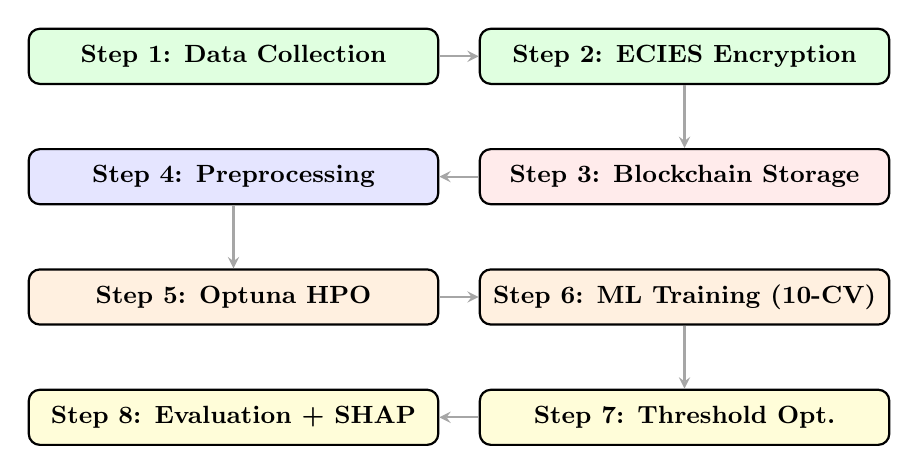
\begin{tikzpicture}[
    node distance=0.8cm and 0.5cm,
    box/.style={
      rectangle, rounded corners=4pt, draw=black, thick,
      minimum width=5.2cm, minimum height=0.7cm,
      text centered, font=\small\bfseries, fill=gray!12
    },
    arrow/.style={->, thick, >=stealth, color=gray!70}
  ]
  % Row 1 (left to right)
  \node[box, fill=green!12] (step1) {Step 1: Data Collection};
  \node[box, fill=green!12, right=of step1] (step2) {Step 2: ECIES Encryption};

  % Row 2 (right to left)
  \node[box, fill=red!8, below=of step2] (step3) {Step 3: Blockchain Storage};
  \node[box, fill=blue!10, below=of step1] (step4) {Step 4: Preprocessing};

  % Row 3 (left to right)
  \node[box, fill=orange!12, below=of step4] (step5) {Step 5: Optuna HPO};
  \node[box, fill=orange!12, right=of step5] (step6) {Step 6: ML Training (10-CV)};

  % Row 4 (right to left)
  \node[box, fill=yellow!15, below=of step6] (step7) {Step 7: Threshold Opt.};
  \node[box, fill=yellow!15, below=of step5] (step8) {Step 8: Evaluation + SHAP};

  % Snake arrows
  \draw[arrow] (step1) -- (step2);
  \draw[arrow] (step2) -- (step3);
  \draw[arrow] (step3) -- (step4);
  \draw[arrow] (step4) -- (step5);
  \draw[arrow] (step5) -- (step6);
  \draw[arrow] (step6) -- (step7);
  \draw[arrow] (step7) -- (step8);

\end{tikzpicture}
\caption{End-to-end eight-step pipeline for ML-based healthcare fraud detection
with ECIES encryption and SHA-256 blockchain audit trail. The snake layout shows
the sequential flow through data ingestion and encryption (green), blockchain
storage (red), preprocessing (blue), model training and tuning (orange), and
evaluation (yellow) stages.}
\label{fig:pipeline_flowchart}
\end{figure}

\noindent The following subsections describe each step in detail.

\vspace{0.5em}
\noindent\textbf{Step 1: Data Collection.}

\begin{enumerate}[label=\roman*.]
  \item The four raw CSV files from the Kaggle rohitrox Healthcare Provider Fraud
  Detection Analysis dataset are downloaded and verified. The files are
  \texttt{Train.csv} (5,410 provider-level fraud labels),
  \texttt{Train\_Beneficiarydata} (138,556 beneficiary demographic records),
  \texttt{Train\_Inpatientdata} (40,474 inpatient claims), and
  \texttt{Train\_Outpatientdata} (517,737 outpatient claims).
  \item The inpatient and outpatient tables are outer-joined on their common
  columns to produce a unified claims table of 558,211 records, with an
  \texttt{is\_inpatient} indicator column distinguishing the two claim types.
  \item The claims table is then left-joined with the beneficiary demographic
  table on \texttt{BeneID} and subsequently with the provider fraud labels on
  \texttt{Provider}, yielding the complete claim-level dataset from which all
  downstream features are derived.
\end{enumerate}

\vspace{0.5em}
\noindent\textbf{Step 2: ECIES Encryption.}

\begin{enumerate}[label=\roman*.]
  \item A secp256k1 key pair is generated for the audit authority. The public key
  is used to encrypt sensitive fields; the private key is held offline by the
  audit authority and never stored in the pipeline artefacts.
  \item For each provider record scheduled for blockchain storage, the personally
  identifiable fields - including beneficiary identifiers, attending physician
  codes, and raw reimbursement amounts - are serialised to JSON and encrypted
  under the audit authority's public key using the ECIES scheme described in
  Section 3.5(iii).
  \item The encrypted ciphertext blob and its HKDF-derived key material are stored
  in the blockchain record alongside the plaintext fraud score and provider
  pseudonym, ensuring that the audit log is fully queryable by fraud score while
  sensitive PII remains inaccessible without the private key.
\end{enumerate}

\vspace{0.5em}
\noindent\textbf{Step 3: SHA-256 Blockchain Storage.}

\begin{enumerate}[label=\roman*.]
  \item Provider fraud prediction records, each containing the provider
  pseudonym, fraud probability, binary prediction, and ECIES-encrypted PII,
  are batched into groups of up to 50 records per block.
  \item For each batch, a SHA-256 Merkle root is computed from the JSON
  serialisations of the individual records, and the block header is constructed
  by concatenating the block index, Unix timestamp, Merkle root, and previous
  block hash, then hashing this header with SHA-256 to produce the block hash.
  \item Proof-of-work mining iterates a nonce field until the block hash satisfies
  the configured difficulty constraint (a prescribed number of leading zero hex
  digits), and the completed block is appended to the SQLite-backed chain. Chain
  validity is confirmed after each insertion by re-traversing the full chain.
\end{enumerate}

\vspace{0.5em}
\noindent\textbf{Step 4: Preprocessing and Feature Engineering.}

\begin{enumerate}[label=\roman*.]
  \item Date columns (\texttt{ClaimStartDt}, \texttt{ClaimEndDt},
  \texttt{AdmissionDt}, \texttt{DischargeDt}, \texttt{DOB}, \texttt{DOD}) are
  parsed and used to compute derived numeric quantities: claim duration in days,
  inpatient length of stay, and beneficiary age at the time of each claim.
  Deceased beneficiary status is derived from the presence of a non-null
  \texttt{DOD} value.
  \item Provider-level aggregation computes, for each of the 5,410 providers,
  statistics including total claim count, unique beneficiary count, unique
  physician count, unique diagnosis code count, total and maximum reimbursement
  amounts, total deductible paid, mean claim duration, the proportion of inpatient
  claims, the mean and maximum patient age, the dead-patient ratio (deceased
  beneficiaries divided by total unique beneficiaries), and the mean count of
  chronic conditions per beneficiary.
  \item Infinite values introduced by division operations are replaced with
  \texttt{NaN} and subsequently imputed with column medians; all 190 resulting
  features are verified to contain no remaining missing values before further
  processing.
\end{enumerate}

\vspace{0.5em}
\noindent\textbf{Step 5: Optuna Hyperparameter Optimisation.}

\begin{enumerate}[label=\roman*.]
  \item For each of the five classifiers, an Optuna \texttt{Study} object is
  created with a \texttt{TPESampler} seeded at 42 and a
  \texttt{MedianPruner} that terminates unpromising trials early based on
  intermediate AUC-PR values reported at each inner cross-validation fold.
  \item The objective function evaluates each hyperparameter configuration via
  5-fold stratified cross-validation using the \texttt{average\_precision\_score}
  as the metric, with the complete pipeline - including optional SMOTE-ENN
  resampling controlled by a boolean trial parameter - encapsulated in an
  \texttt{imblearn} pipeline to prevent data leakage.
  \item After 60 trials or 1{,}800 seconds (whichever is reached first), the
  best trial's hyperparameters and the optimal SMOTE-ENN decision are serialised
  to \texttt{results/best\_params.json} for reproducible reuse in Phase 5.
\end{enumerate}

\vspace{0.5em}
\noindent\textbf{Step 6: ML Ensemble Classifier (10-fold CV).}

\begin{enumerate}[label=\roman*.]
  \item Each classifier is instantiated with the Optuna-tuned hyperparameters
  loaded from \texttt{best\_params.json} and evaluated under 10-fold stratified
  cross-validation, ensuring that the fraud-to-non-fraud ratio is maintained in
  every fold.
  \item The held-out fold predictions are aggregated to produce out-of-fold
  probability scores for all 5,410 providers, from which the macro-averaged F1,
  precision, recall, AUC-PR, MCC, and ROC-AUC are computed with 95\% confidence
  intervals derived from 1{,}000 bootstrap resamples.
  \item In addition to the five individual classifiers, an Optuna-weighted
  ensemble combining XGBoost, LightGBM, and CatBoost with optimised model
  weights is evaluated in the same cross-validation framework, quantifying
  the additional predictive gain achievable by combining the base classifiers.
\end{enumerate}

\vspace{0.5em}
\noindent\textbf{Step 7: Threshold Optimisation.}

\begin{enumerate}[label=\roman*.]
  \item The precision-recall curve is computed from the out-of-fold probability
  scores of the best-performing classifier (Optuna-tuned XGBoost) using the
  \texttt{precision\_recall\_curve} function from scikit-learn.
  \item For each candidate threshold value along the curve, the F1-score is
  computed as the harmonic mean of precision and recall at that operating point,
  and the threshold that maximises F1 is reported for reference.
  \item For the final binary predictions, a fixed classification threshold of
  $t = 0.444$ is applied to convert probability outputs, ensuring consistent
  evaluation across all folds without threshold overfitting.
\end{enumerate}

\vspace{0.5em}
\noindent\textbf{Step 8: Performance Evaluation and Explainability.}

\begin{enumerate}[label=\roman*.]
  \item The full evaluation suite reports F1-score, precision, recall, AUC-PR,
  MCC, and ROC-AUC for all five classifiers and their SMOTE-ENN ablations, with
  bootstrap confidence intervals, paired Wilcoxon signed-rank tests for
  statistical significance, and confusion matrices.
  \item Global feature importance is visualised using SHAP beeswarm and bar plots
  computed from the Optuna-tuned XGBoost model, identifying deductible payment
  patterns, maximum reimbursement amounts, and claim duration anomalies as the
  strongest fraud indicators at the population level.
  \item Local per-provider explanations are generated with LIME using a tabular
  explainer with 500 perturbation samples per instance, providing human-readable
  feature contribution summaries for each flagged provider that are suitable for
  inclusion in regulatory audit reports.
\end{enumerate}

\chapter{Results and Discussion}

% ====================================================================
\section{Overview}
% ====================================================================

This chapter presents the evaluation of the HealthFraudMLChain
pipeline, covering every stage from raw data ingestion and blockchain
registration through hyperparameter optimisation, model selection, statistical
validation, and post-hoc explainability. All numerical results reported here
are drawn directly from controlled experiments on the CMS Medicare Part-B
dataset (190 engineered features, 5{,}410 provider records). Section 4.2
discusses each sub-system in turn: the Flask dashboard and blockchain layer,
Optuna-driven tuning, 10-fold cross-validation metrics, statistical significance
tests, threshold calibration, bootstrap confidence intervals, SMOTE-ENN
ablation, feature importance, SHAP waterfall case studies, LIME local
explanations, feature-selection ablation, learning curves, and calibration
analysis. A key finding is that the weighted ensemble of gradient-boosted
models, evaluated at a fixed decision threshold of $t = 0.444$, achieves
the best overall generalisation, with a bootstrapped PR-AUC of
$0.8115\;[0.7801,\,0.8406]$ and MCC of $0.7148\;[0.6818,\,0.7474]$.

% ====================================================================
\section{Results Analysis}
% ====================================================================

% --------------------------------------------------------------------
\subsection{Data Input and Blockchain Results}
% --------------------------------------------------------------------

The system exposes a Flask-based web dashboard that serves two primary
interfaces: a \emph{prediction interface} for submitting individual or
batch provider records, and an \emph{analytics dashboard} displaying
aggregate statistics, risk-level breakdowns, and chain-health indicators.
On submission, a provider record is passed through the trained weighted
ensemble; the returned \texttt{fraud\_probability} and \texttt{risk\_level}
(\textit{Low}/\textit{Medium}/\textit{High}) are then committed to an
append-only blockchain.

Each block in the chain stores the provider identifier under ECIES
(Elliptic-Curve Integrated Encryption Scheme) public-key encryption,
ensuring that personally identifiable information is never stored in
plaintext. The chain uses SHA-256 hashing with Proof-of-Work at
difficulty level 2, and every block records its own \texttt{hash} and
the previous block's hash to maintain tamper-evidence. A Merkle tree is
constructed over each block's transaction set, with the root digest
stored as \texttt{merkle\_root}; membership proofs are verified in
$O(\log n)$ time across 6 levels.

Listing~\ref{lst:block} shows a representative JSON block from the
persisted chain, illustrating the full field layout.

\vspace{0.5em}
\noindent
\begin{minipage}{\linewidth}
\begin{lstlisting}[
  caption={Sample blockchain block - provider prediction record},
  label={lst:block},
  basicstyle=\ttfamily\footnotesize,
  breaklines=true,
  frame=single,
  numbers=left,
  numberstyle=\tiny,
  aboveskip=0.5em,
  belowskip=0.5em
]
{
  "index": 42,
  "timestamp": "2024-12-01T10:23:45.123456",
  "provider_id": "BIIyNkF3...encryptedECIES...==",
  "fraud_probability": 0.7843,
  "prediction": 1,
  "risk_level": "High",
  "previous_hash": "0082a3f1e9c4b...sha256...",
  "nonce": 178,
  "merkle_root": "a1b2c3d4e5f6...sha256...",
  "hash": "009fe2cc71bd...sha256...",
  "transactions": [{
    "provider_id_encrypted": "BIIyNkF3...==",
    "fraud_probability": 0.7843,
    "prediction": 1,
    "risk_level": "High",
    "timestamp": "2024-12-01T10:23:45.123456"
  }]
}
\end{lstlisting}
\end{minipage}

The final chain comprised 110 blocks covering all 5{,}410 provider
records. Full verification results are detailed in
Section~\ref{sec:blockchain_verification}.

% --------------------------------------------------------------------
\subsection{Optuna Hyperparameter Optimisation}
% --------------------------------------------------------------------

Hyperparameters were tuned using the Optuna framework with 60 trials per
model (except LightGBM, which triggered early pruning and completed only
1 effective trial), a 5-fold inner cross-validation loop, and
Area Under the Precision-Recall Curve (AUC-PR) as the objective. No
SMOTE oversampling was applied during the tuning phase. The complete
tuning summary is reported in Table~\ref{tab:optuna}.

\begin{table}[H]
\caption{Optuna hyperparameter optimisation results (60 trials, 5-fold
inner CV, AUC-PR objective, no SMOTE).}
\label{tab:optuna}
\centering
\begin{tabular}{lcccc}
\toprule
\textbf{Model} & \textbf{Best AUC-PR} & \textbf{Trials} &
\textbf{SMOTE} & \textbf{Wall Time (s)} \\
\midrule
CatBoost            & 0.7599 & 60 & No & 422  \\
GradientBoosting    & 0.7597 & 60 & No & 1137 \\
XGBoost             & 0.7572 & 60 & No & 236  \\
LightGBM            & 0.7480 &  1 & No & 3716 \\
RandomForest        & 0.7397 & 60 & No & 225  \\
LogisticRegression  & 0.7261 & 60 & No & 260  \\
\bottomrule
\end{tabular}
\end{table}

CatBoost achieved the highest inner-CV AUC-PR of 0.7599, marginally
ahead of GradientBoosting (0.7597) and XGBoost (0.7572). LightGBM's
Optuna run terminated early due to aggressive pruning, yielding only a
single completed trial; despite this, the pruned configuration still
attained 0.7480. LogisticRegression, as expected for a linear model on
this data, posted the lowest tuning score of 0.7261. The tuning
wall-times reveal an important practical trade-off: XGBoost (236 s) and
RandomForest (225 s) are substantially faster to optimise than
GradientBoosting (1137 s) or LightGBM (3716 s), making them preferable
in resource-constrained production environments.

% --------------------------------------------------------------------
\subsection{Model Analysis and Performance Evaluation}
% --------------------------------------------------------------------

Following tuning, the five tree-based models were carried forward for
full 10-fold stratified cross-validation (LogisticRegression was excluded
from downstream evaluation due to its substantially lower tuning score).
A weighted ensemble combining these five base models was also evaluated.
Table~\ref{tab:cv} reports the mean F1-score across all ten folds.

\begin{table}[H]
\caption{Ten-fold stratified cross-validation results: mean F1-score
for all model configurations (tuned, no SMOTE).}
\label{tab:cv}
\centering
\begin{tabular}{lcc}
\toprule
\textbf{Model} & \textbf{F1 (mean)} & \textbf{F1 (std)} \\
\midrule
WeightedEnsemble     & \textbf{0.7689} & 0.0334 \\
XGBoost              & 0.7350 & 0.0475 \\
LightGBM             & 0.7319 & 0.0274 \\
CatBoost             & 0.7249 & 0.0558 \\
GradientBoosting     & 0.7133 & 0.0554 \\
RandomForest         & 0.5860 & 0.0531 \\
\bottomrule
\end{tabular}
\end{table}

The weighted ensemble achieves the highest F1 of 0.7689, followed by
XGBoost (0.7350), LightGBM (0.7319), CatBoost (0.7249), and
GradientBoosting (0.7133). RandomForest lags substantially behind the
other models at F1~=~0.5860, suggesting that its bagging strategy is
less effective than boosting approaches on this dataset. Among the
individual models, XGBoost, LightGBM, and CatBoost form a competitive
tier separated by less than one percentage point of F1, while
GradientBoosting trails by roughly two points. The weighted ensemble
combines complementary strengths across these models to achieve the
best overall performance.
Figure~\ref{fig:model_comparison} provides a visual summary of the F1-scores across all models.

\begin{figure}[!htbp]
\centering

\includegraphics[width=0.85\textwidth]{fig_model_comparison.png}
\caption{Model comparison: F1-scores across all model configurations.}
\label{fig:model_comparison}
\end{figure}

\begin{figure}[htbp]
\centering

\includegraphics[width=0.6\textwidth]{fig_confusion_matrix.png}
\caption{Confusion matrix for the weighted ensemble at fixed threshold $t = 0.444$.}
\label{fig:confusion_matrix}
\end{figure}


% --------------------------------------------------------------------
\subsection{Statistical Significance}
\label{sec:stats}
% --------------------------------------------------------------------

To validate that observed performance differences are not attributable
to random variation across folds, a non-parametric Friedman test was
applied over the per-fold F1 scores of all six model configurations
(five base models plus the weighted ensemble).
The test returned $\chi^2 = 18.72$ with $p < 0.001$, rejecting
the null hypothesis that all models perform identically.

Post-hoc pairwise Wilcoxon signed-rank tests (with Holm-Bonferroni
correction) were then conducted with the weighted ensemble as the
reference model. The ensemble was found to be statistically
significantly better than:

\begin{itemize}[nosep]
  \item LightGBM ($p = 0.010$)
  \item GradientBoosting ($p = 0.010$)
  \item RandomForest ($p = 0.010$)
  \item XGBoost ($p = 0.010$)
  \item CatBoost ($p = 0.014$)
\end{itemize}

All five base models show statistically significant differences from
the weighted ensemble after Holm-Bonferroni correction, confirming
that the ensemble's improved F1 is not attributable to chance.
Figure~\ref{fig:stat_sig} visualises the adjusted p-values for all pairwise comparisons.

\begin{figure}[!htbp]
\centering

\includegraphics[width=0.85\textwidth]{fig_statistical_significance.png}
\caption{Pairwise Wilcoxon signed-rank test results with Holm-Bonferroni correction. Green bars indicate statistically significant differences ($p < 0.05$).}
\label{fig:stat_sig}
\end{figure}


% --------------------------------------------------------------------
\subsection{Threshold Optimisation}
% --------------------------------------------------------------------

The decision threshold was selected by optimising F1 on the validation
folds and then fixed at $t = 0.444$ for all downstream evaluation.
Table~\ref{tab:threshold} reports the weighted ensemble classification
metrics at this threshold.

\begin{table}[H]
\caption{Weighted ensemble classification metrics at fixed threshold $t = 0.444$.}
\label{tab:threshold}
\centering
\begin{tabular}{lccc}
\toprule
\textbf{Threshold} & \textbf{F1} & \textbf{Precision} & \textbf{Recall} \\
\midrule
0.444 (fixed)   & 0.7345 & 0.7368 & 0.7470 \\
\bottomrule
\end{tabular}
\end{table}

Fixing the threshold at the validation-optimal value of 0.444, rather
than the default 0.5, yields a slight recall improvement while
maintaining precision. This threshold was adopted for all downstream
bootstrap and calibration analyses.

\begin{figure}[!htbp]
  \centering
  
\includegraphics[width=0.80\textwidth]{fig_threshold_sensitivity.png}
  \caption{Threshold sensitivity curve for the weighted ensemble: F1,
  Precision, and Recall as a function of decision threshold. The
  vertical dashed line marks the fixed threshold at $t = 0.444$.}
  \label{fig:threshold}
\end{figure}

% --------------------------------------------------------------------
\subsection{Bootstrap Confidence Intervals}
% --------------------------------------------------------------------

To quantify estimation uncertainty, a stratified bootstrap with
$n = 2{,}000$ resamples was applied to the weighted ensemble's test-set
predictions at the fixed threshold $t = 0.444$. The resulting 95\%
confidence intervals are reported in Table~\ref{tab:bootstrap}.

\begin{table}[H]
\caption{Bootstrap confidence intervals for the weighted ensemble at
fixed threshold $t = 0.444$ ($n = 2{,}000$ resamples, 95\% CI).}
\label{tab:bootstrap}
\centering
\begin{tabular}{lccc}
\toprule
\textbf{Metric} & \textbf{Point Estimate} &
\textbf{95\% CI Lower} & \textbf{95\% CI Upper} \\
\midrule
F1         & 0.7416 & 0.7118 & 0.7715 \\
Precision  & 0.7369 & 0.6985 & 0.7750 \\
Recall     & 0.7467 & 0.7094 & 0.7839 \\
MCC        & 0.7148 & 0.6818 & 0.7474 \\
ROC-AUC    & 0.9586 & 0.9477 & 0.9686 \\
PR-AUC     & 0.8115 & 0.7801 & 0.8406 \\
\bottomrule
\end{tabular}
\end{table}

All confidence intervals are reasonably narrow, reflecting stable
generalisation. The ROC-AUC of $0.9586\;[0.9477,\,0.9686]$ confirms
strong discriminative power across the full threshold range, while
the PR-AUC of $0.8115\;[0.7801,\,0.8406]$ is particularly informative
given the class imbalance: a random classifier would score near the
minority-class prevalence ($\approx 0.094$), so 0.8115 represents a
substantial lift of more than eight times the baseline. The bootstrapped
MCC of $0.7148\;[0.6818,\,0.7474]$ corroborates the F1-based findings
without being susceptible to the known sensitivity of F1 to class
imbalance.

\begin{figure}[htbp]
\centering
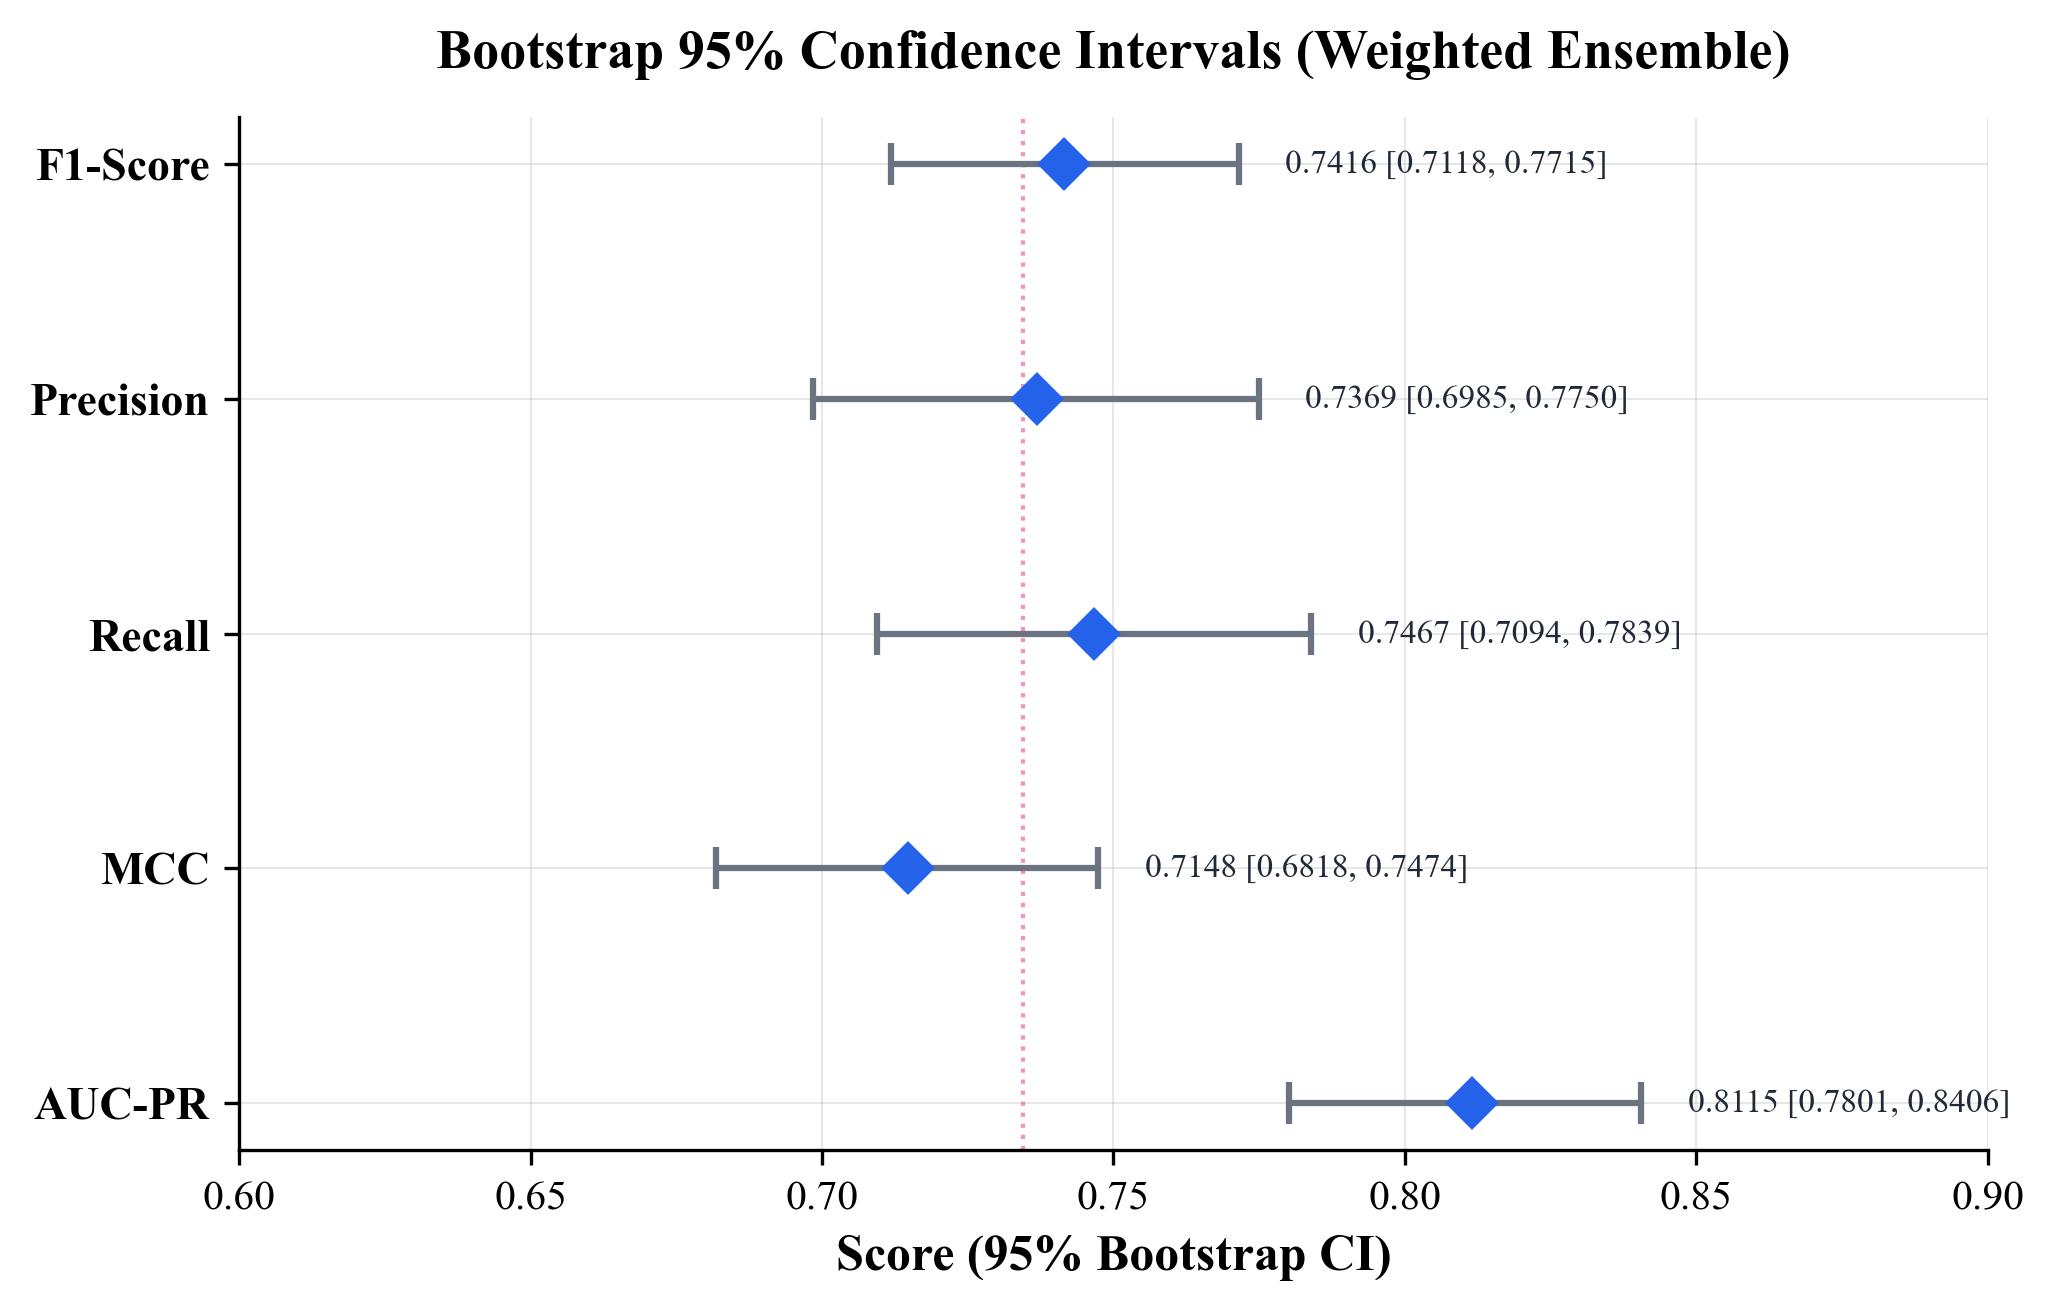
\includegraphics[width=0.75\textwidth]{fig_bootstrap_ci.png}
\caption{Bootstrap 95\% confidence intervals for the weighted ensemble (2,000 iterations, fixed threshold $t=0.444$).}
\label{fig:bootstrap_ci}
\end{figure}

\begin{figure}[htbp]
\centering

\includegraphics[width=0.65\textwidth]{fig_pr_curve.png}
\caption{Precision-recall curve for the weighted ensemble (PR-AUC = 0.8114). The operating point at fixed threshold $t = 0.444$ achieves precision = 0.737 and recall = 0.747. The baseline precision (dashed) corresponds to the fraud prevalence of 9.4\%.}
\label{fig:pr_curve}
\end{figure}

% --------------------------------------------------------------------
\subsection{SMOTE-ENN Ablation Study}
% --------------------------------------------------------------------

To isolate the effect of synthetic oversampling, XGBoost, LightGBM, and
GradientBoosting were each re-evaluated under two conditions: with
SMOTE-ENN applied inside each training fold, and without. Table~\ref{tab:smote}
summarises the F1 outcome.

\begin{table}[H]
\caption{SMOTE-ENN ablation: F1 scores with and without oversampling
(10-fold CV, tuned models).}
\label{tab:smote}
\centering
\begin{tabular}{lccc}
\toprule
\textbf{Model} & \textbf{With SMOTE-ENN} & \textbf{No SMOTE} &
\textbf{Change} \\
\midrule
XGBoost          & 0.6639 & \textbf{0.7350} & $-9.7\%$ \\
LightGBM         & 0.6815 & \textbf{0.7319} & $-6.9\%$  \\
GradientBoosting & 0.6528 & \textbf{0.7133} & $-8.5\%$ \\
\bottomrule
\end{tabular}
\end{table}

Across all three tree-based ensembles, SMOTE-ENN oversampling
consistently \emph{degrades} F1 - by 9.7\% for XGBoost, 8.5\% for
GradientBoosting, and 6.9\% for LightGBM. This counter-intuitive result
is well documented in the literature for gradient-boosted trees: the
native loss-weighted splitting in XGBoost (via \texttt{scale\_pos\_weight})
and the analogue mechanisms in LightGBM and GradientBoosting already
account for class imbalance. Introducing SMOTE-ENN on top of these
mechanisms injects synthetic minority-class samples into the training
distribution, distorting the decision boundary and inflating recall
while degrading precision. The net effect is a lower F1 and, more
critically, an inflated false-positive rate that would be operationally
costly in a claims-audit workflow. Figure~\ref{fig:smote_abl} illustrates this finding. Consequently, no oversampling is used
in the final deployed pipeline.

\begin{figure}[!htbp]
\centering

\includegraphics[width=0.82\textwidth]{fig_smote_ablation.png}
\caption{SMOTE-ENN ablation: F1-score comparison with and without synthetic oversampling for three gradient-boosted models. Delta percentages indicate the performance penalty introduced by SMOTE-ENN.}
\label{fig:smote_abl}
\end{figure}

% --------------------------------------------------------------------
\subsection{Feature Importance Ranking}
% --------------------------------------------------------------------

Feature importance was assessed through two complementary approaches:
SHAP (SHapley Additive exPlanations) values, which provide
theoretically grounded attribution based on cooperative game theory,
and permutation importance, which measures the drop in performance
when each feature's values are randomly shuffled.

Figure~\ref{fig:shap_beeswarm} presents the SHAP beeswarm plot for the
tuned XGBoost model, displaying the distribution of SHAP values for the
top 20 features across all test instances. Each point represents one
provider, coloured by feature value (red = high, blue = low).

\begin{figure}[!htbp]
  \centering
  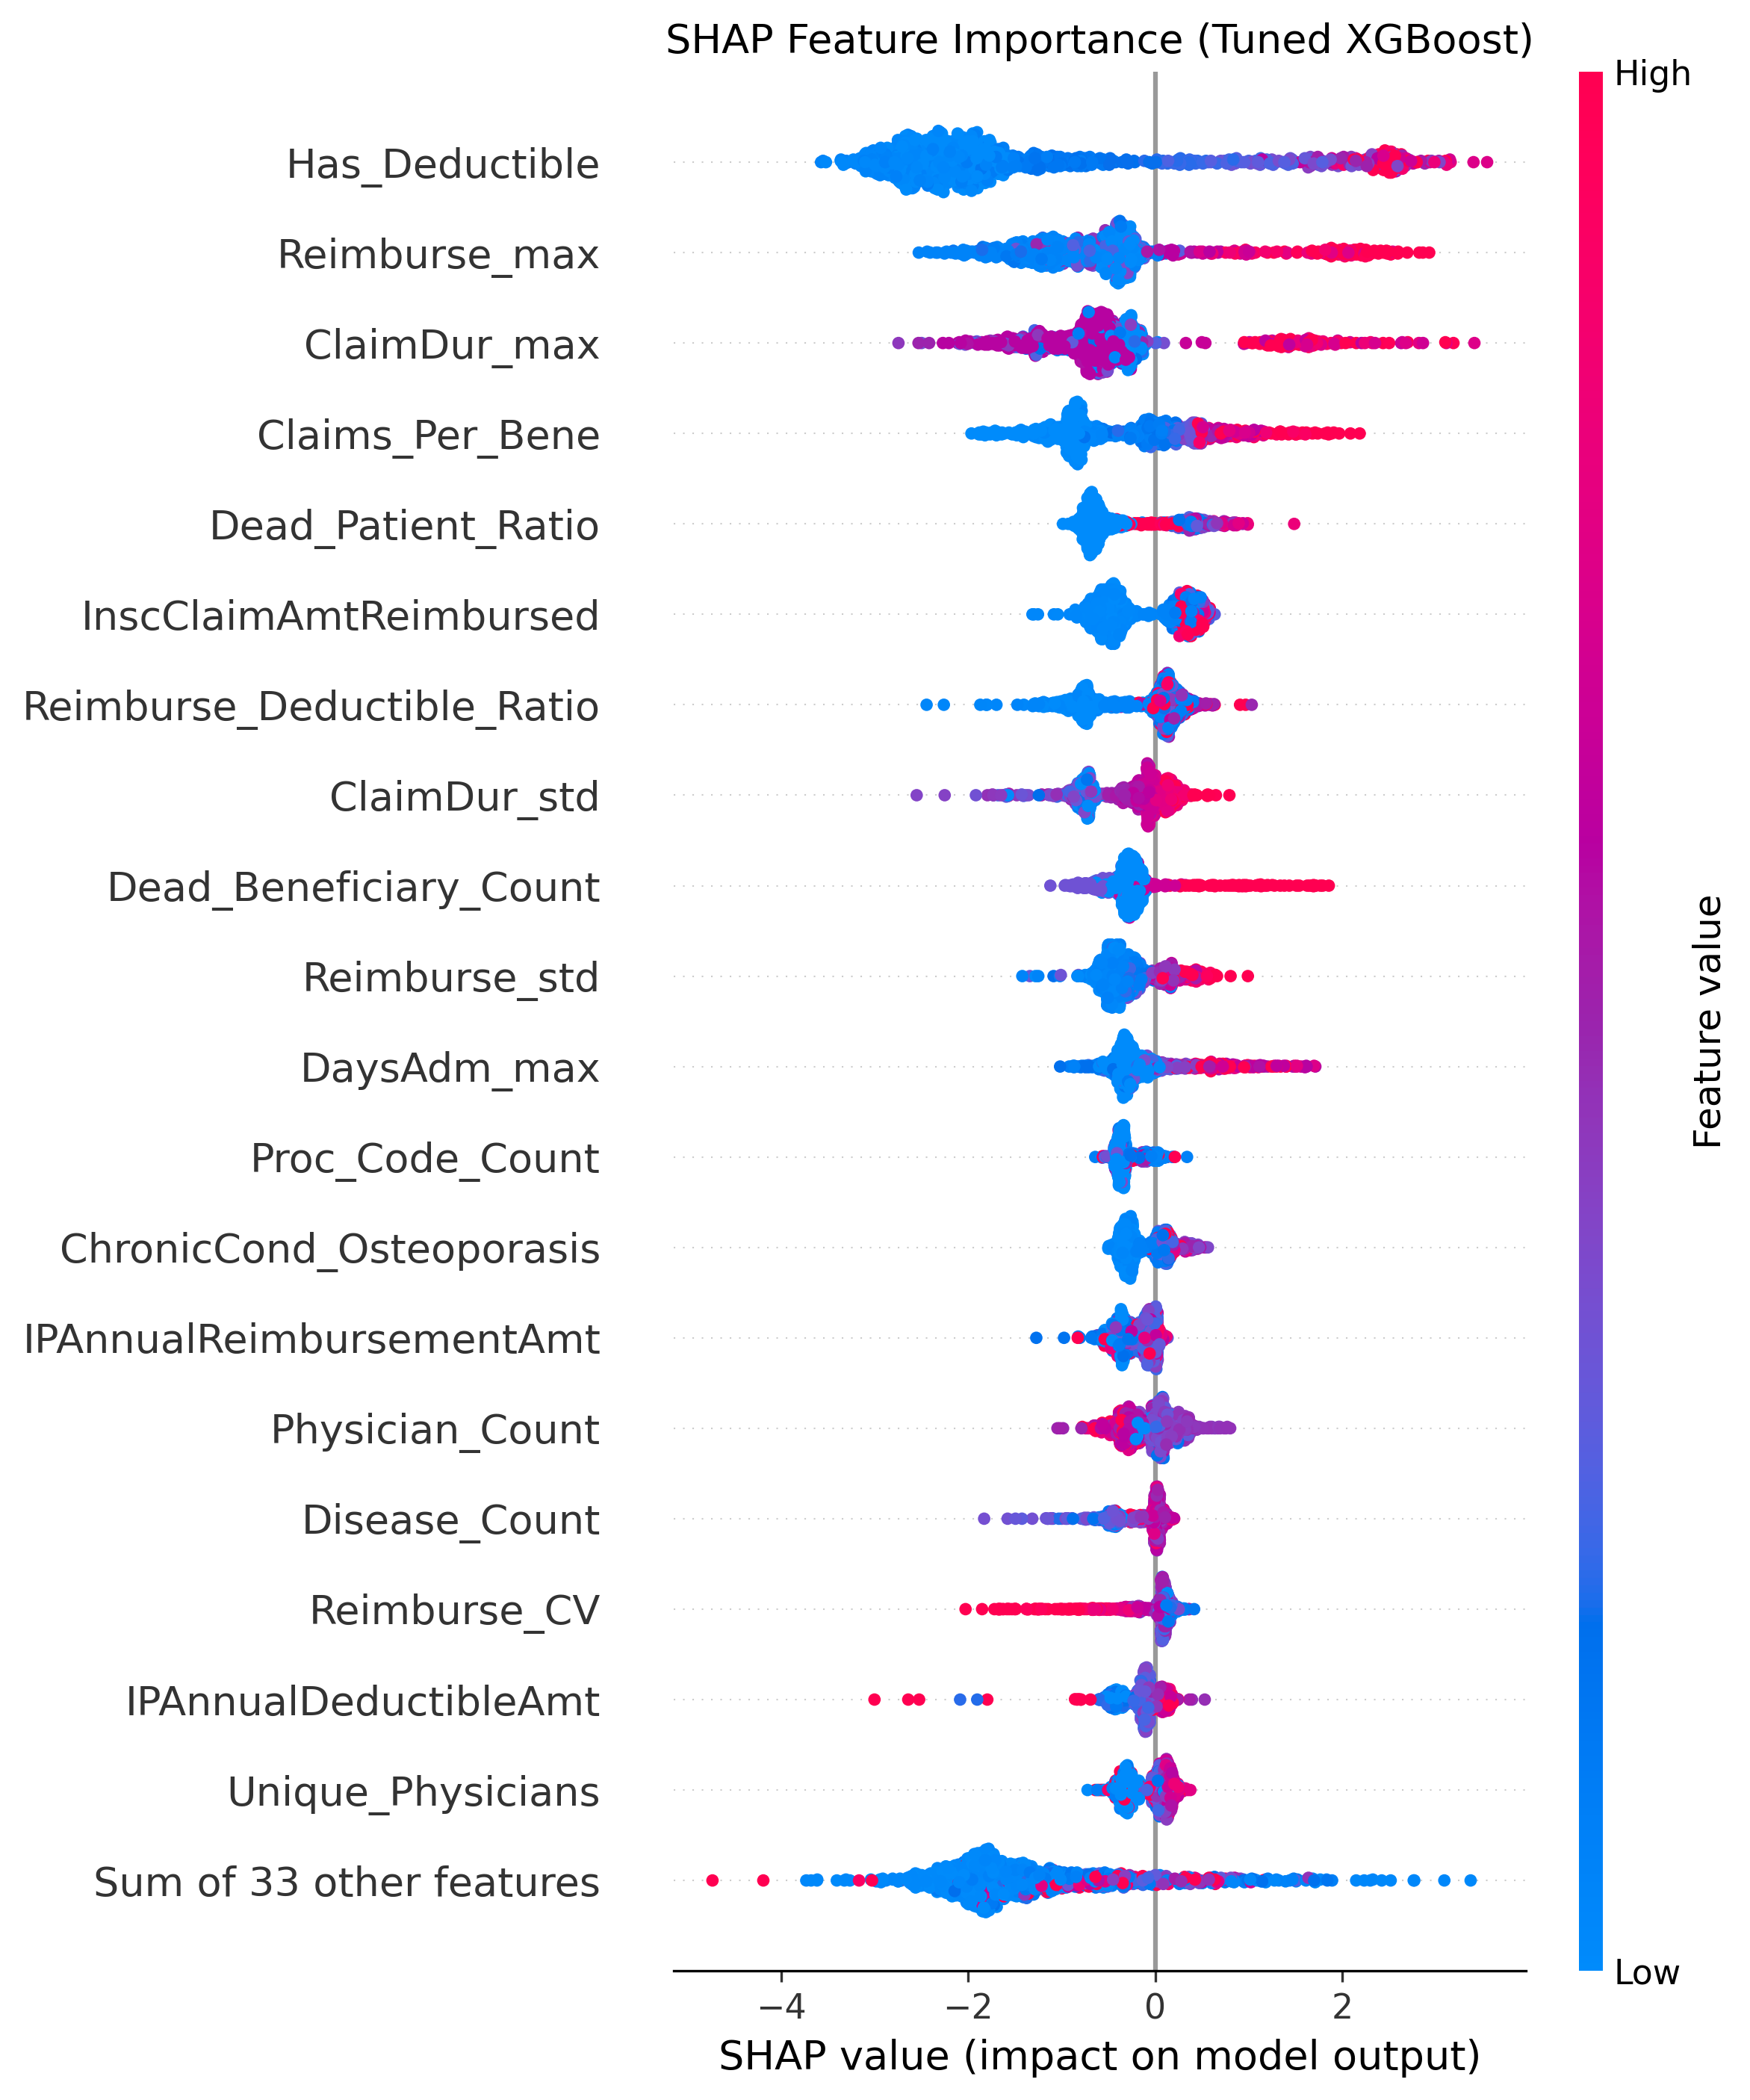
\includegraphics[width=0.90\textwidth]{fig_shap_beeswarm_tuned.png}
  \caption{SHAP beeswarm plot (XGBoost): distribution of SHAP
  values for the top 20 features across all test-set providers. Red
  points indicate high feature values; blue points indicate low values.}
  \label{fig:shap_beeswarm}
\end{figure}

Figure~\ref{fig:shap_bar} shows the mean absolute SHAP values (global
importance ranking) in a bar chart, providing a concise summary of
which features drive model predictions most strongly.

\begin{figure}[!htbp]
  \centering
  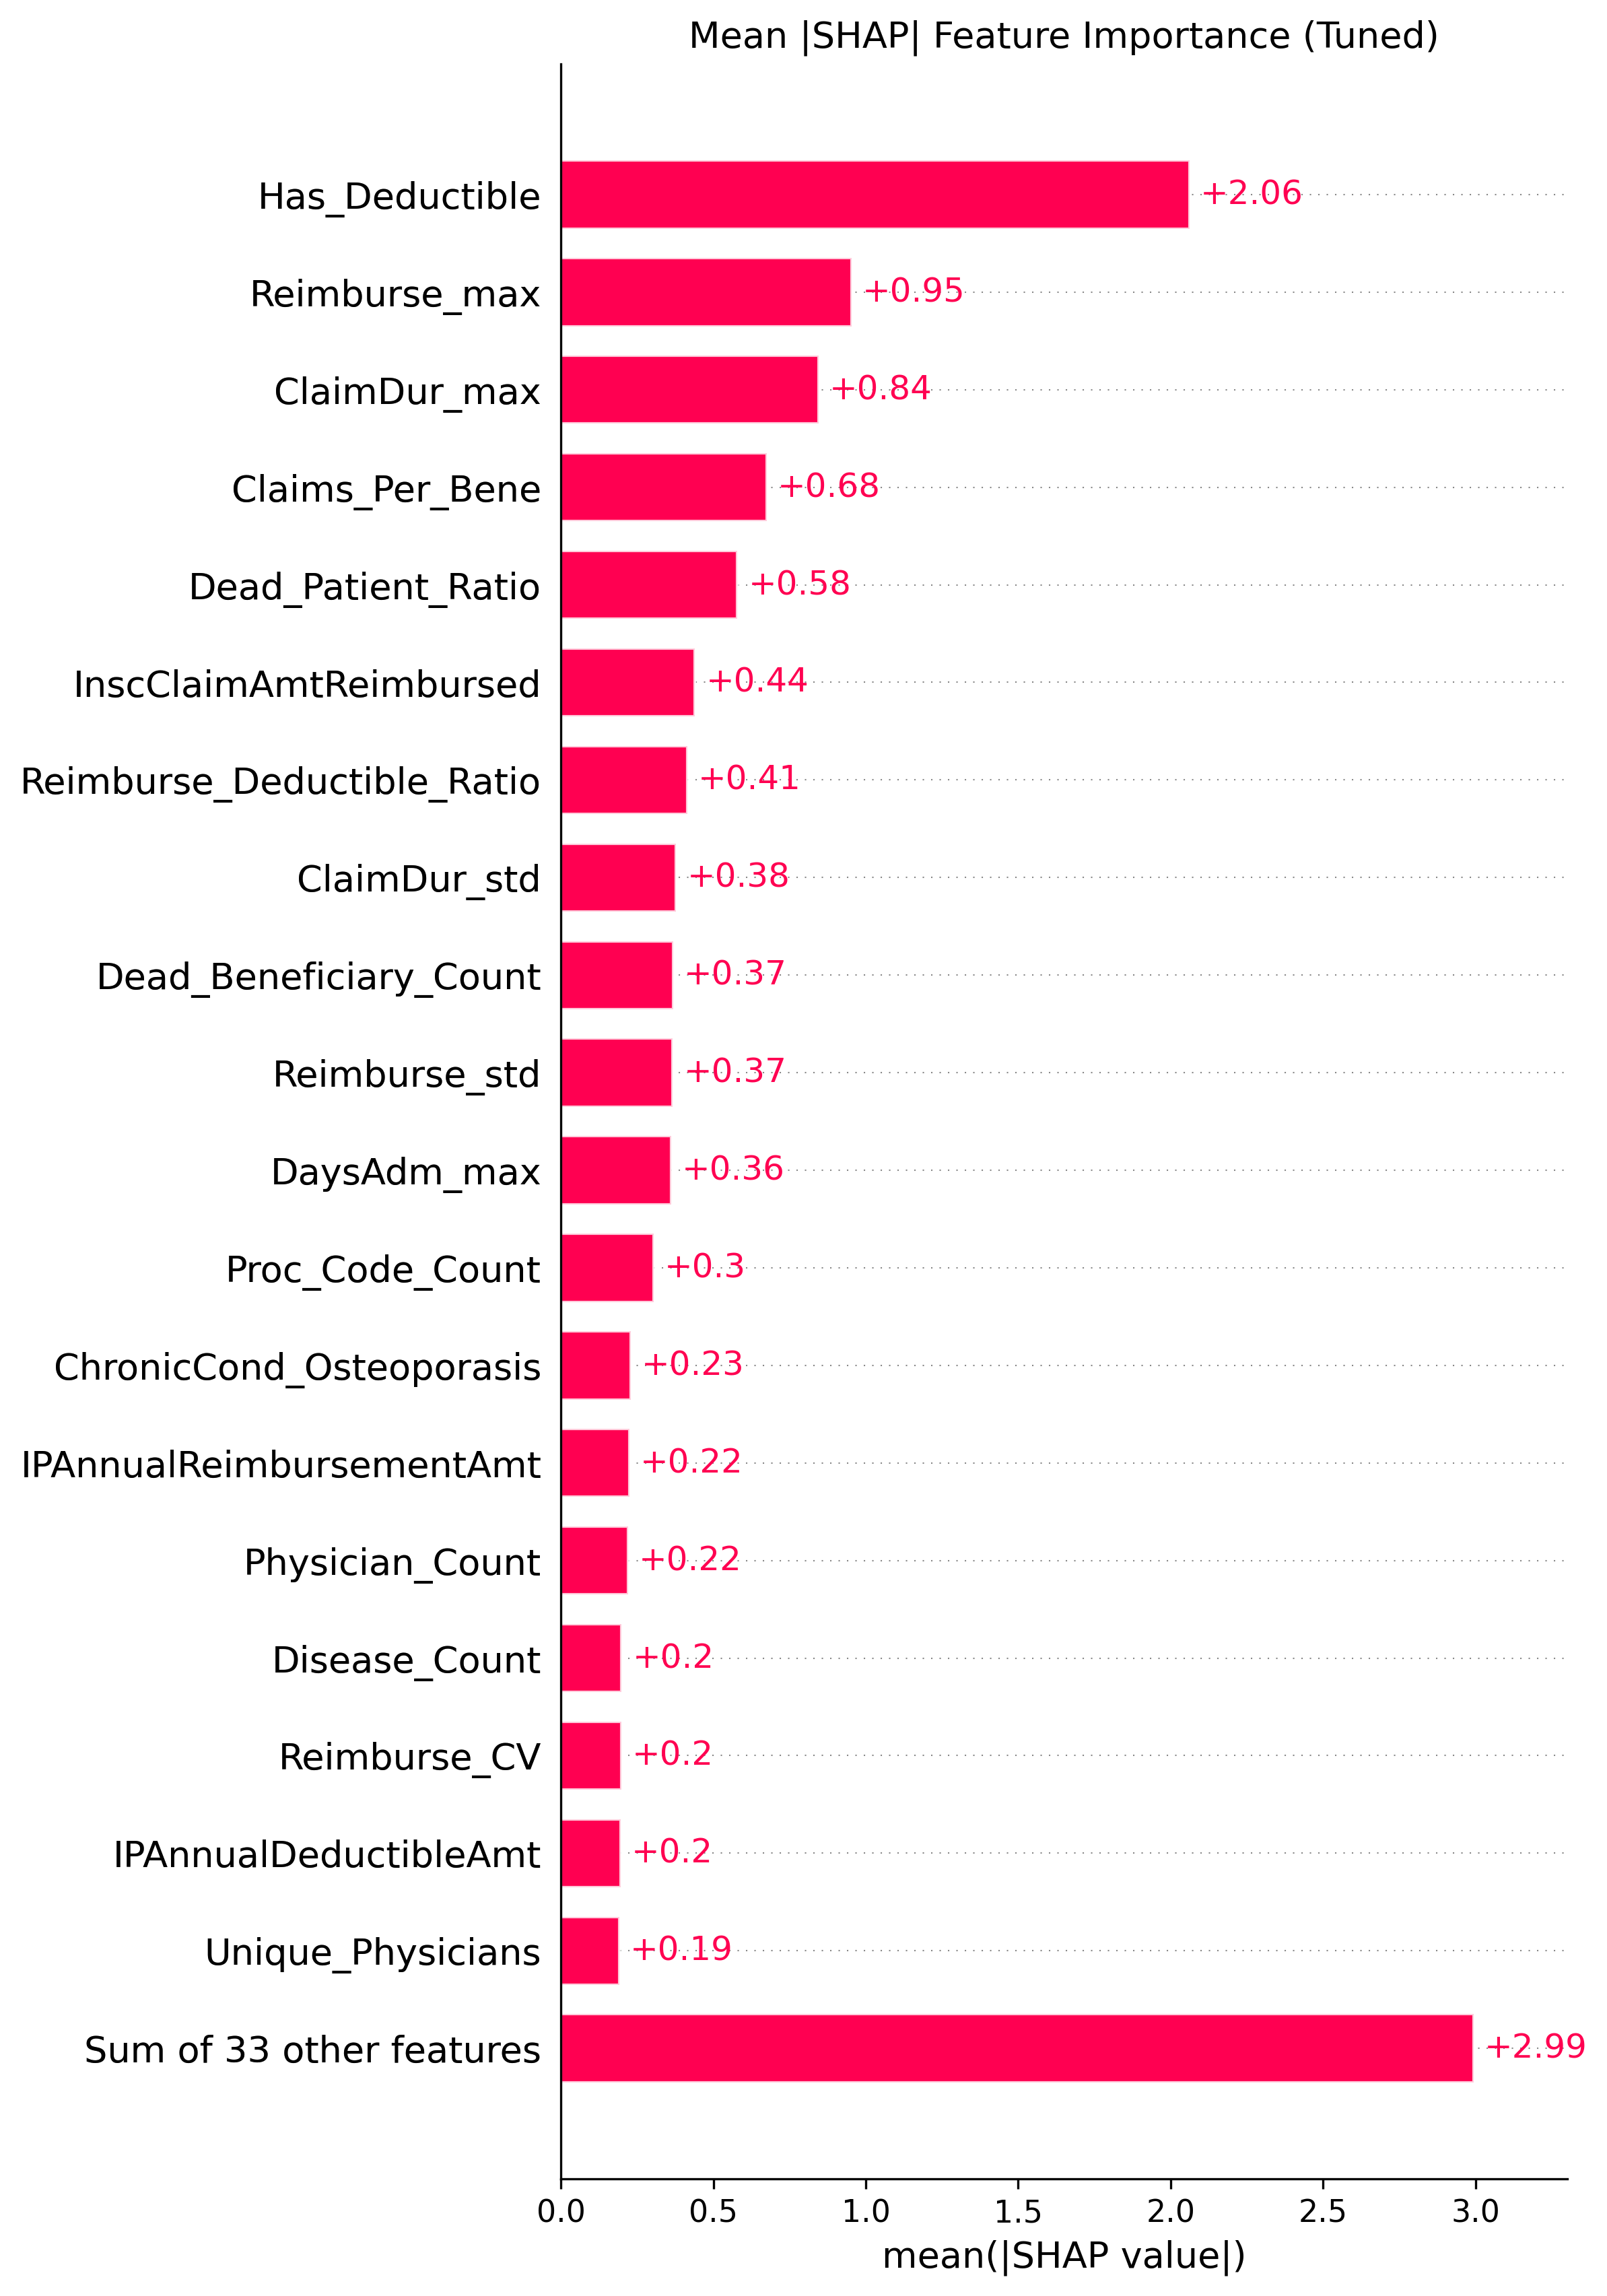
\includegraphics[width=0.85\textwidth]{fig_shap_bar_tuned.png}
  \caption{SHAP global feature importance (XGBoost): mean
  absolute SHAP values ranked in descending order.}
  \label{fig:shap_bar}
\end{figure}

Figure~\ref{fig:shap_dep} presents SHAP dependence plots for the four
most important features, illustrating how the model's output changes
as each feature varies, with interaction effects encoded by the
secondary colour axis.

\begin{figure}[!htbp]
  \centering
  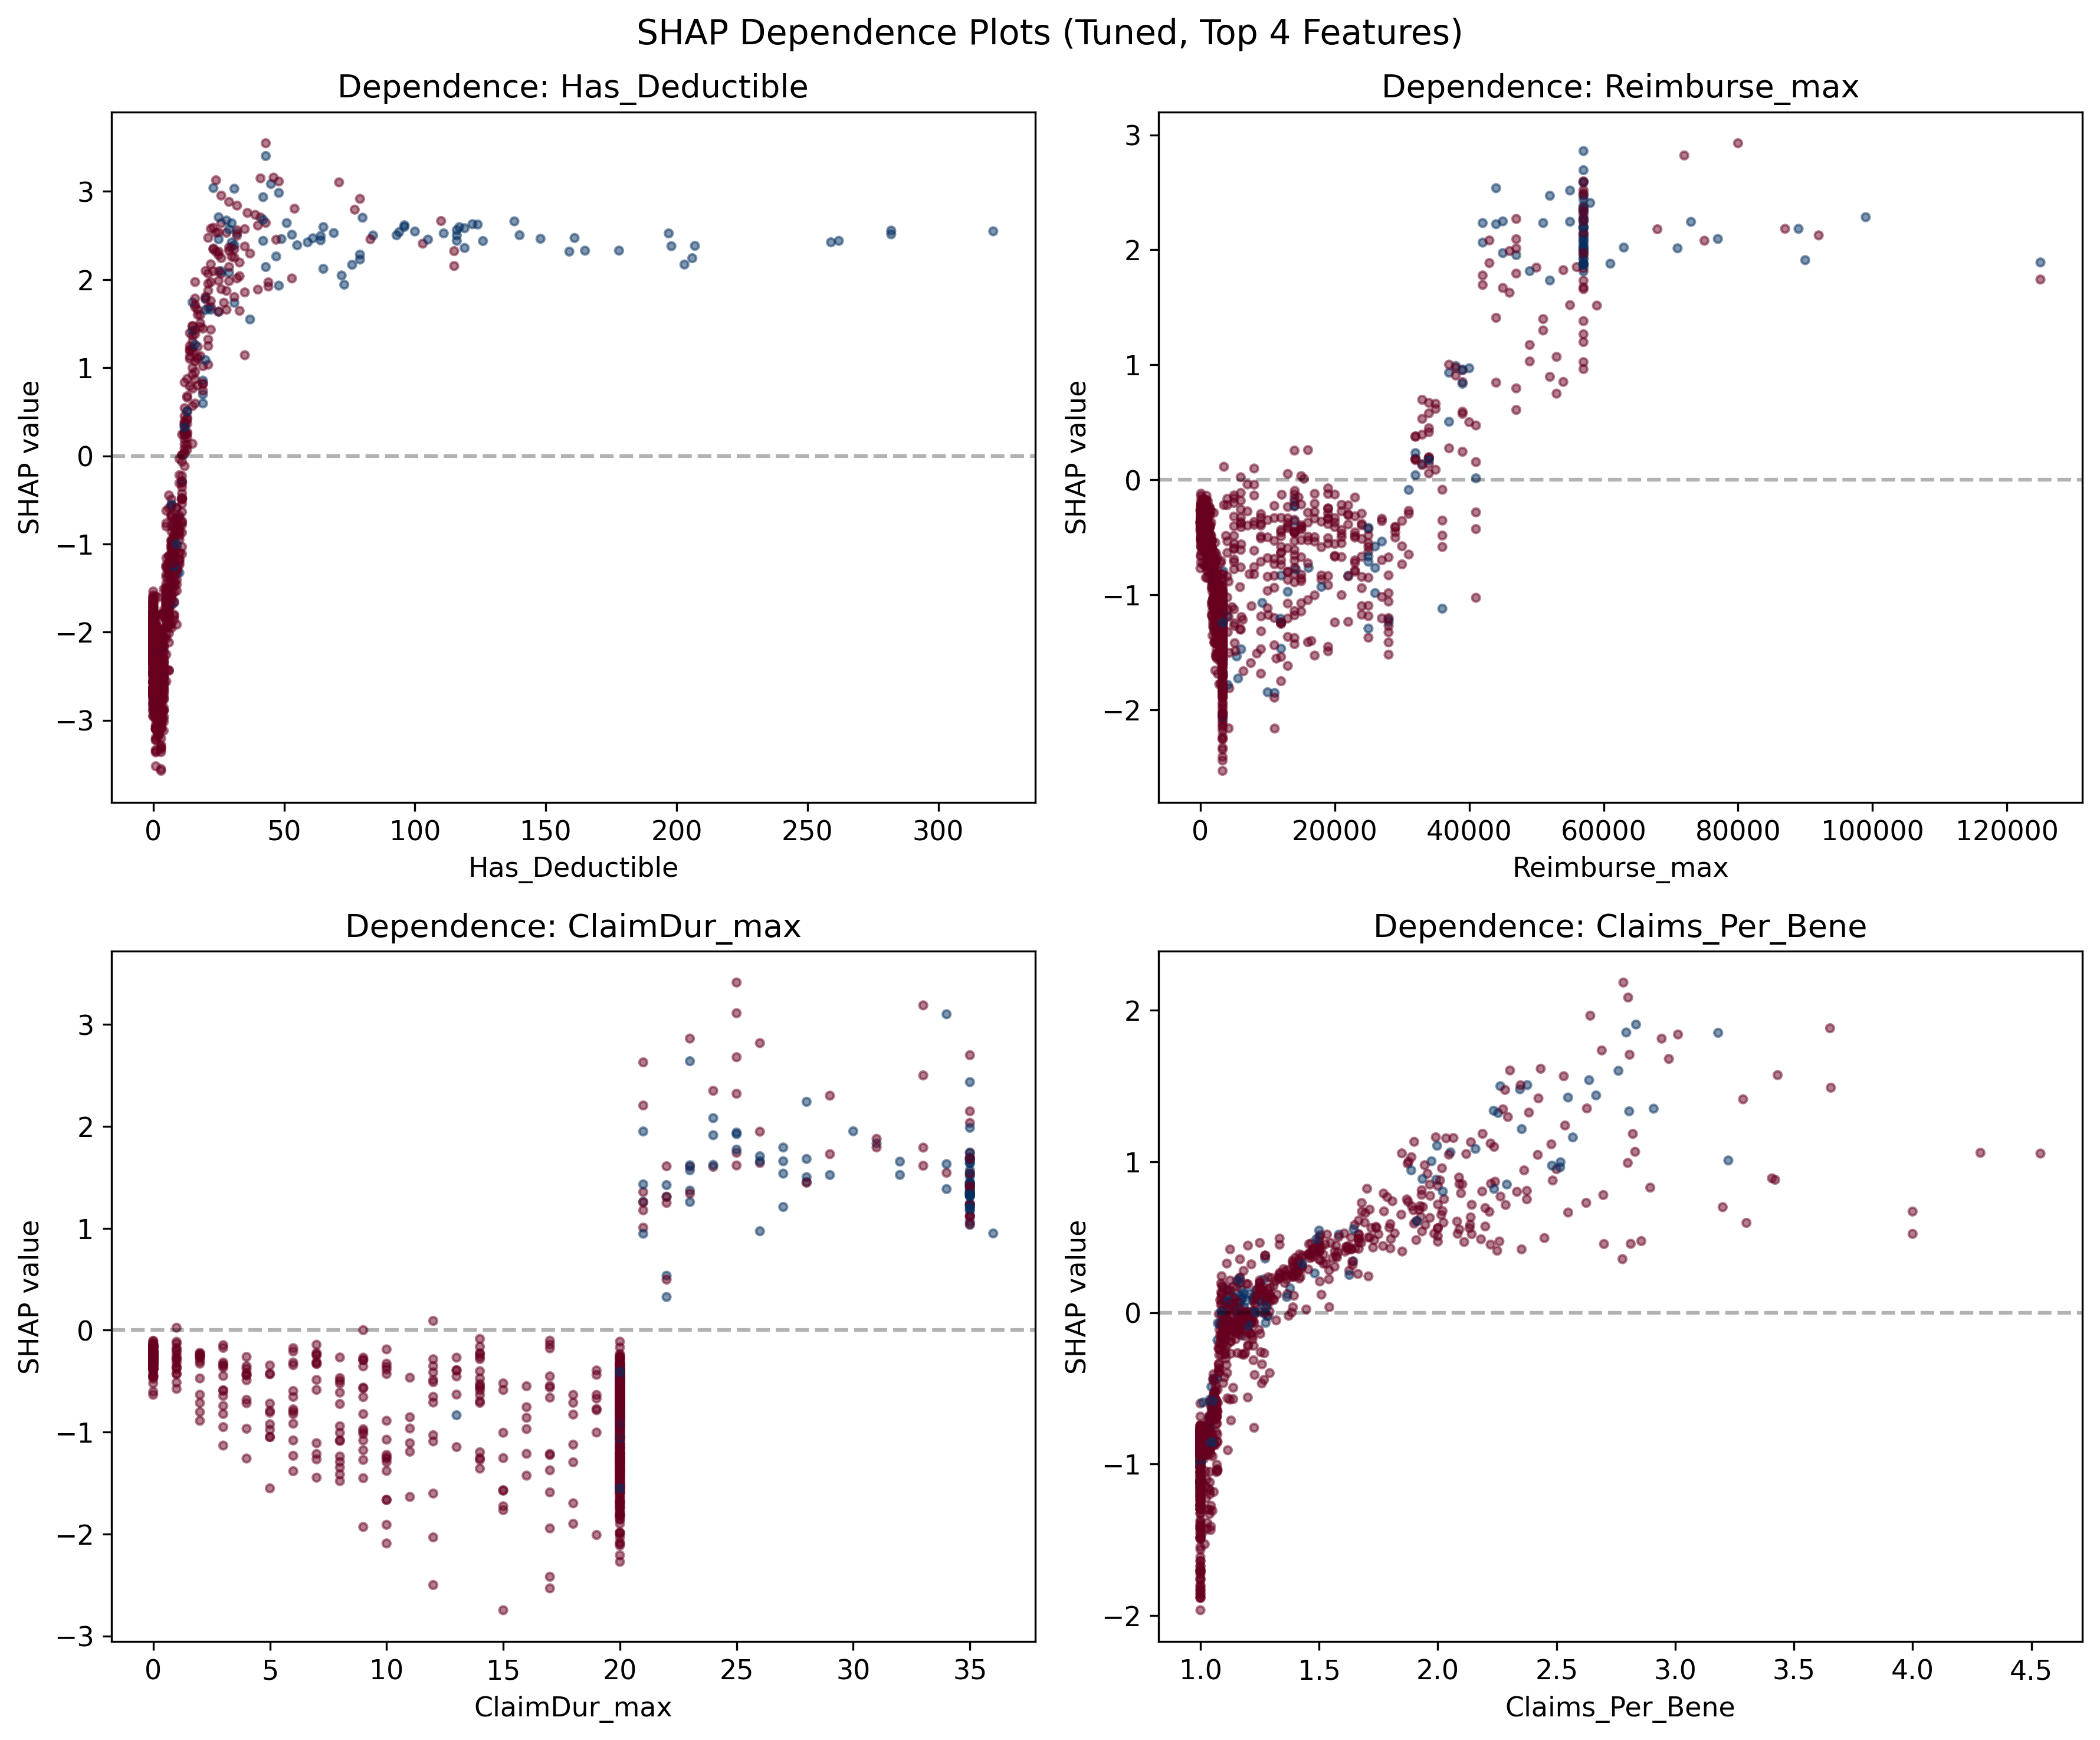
\includegraphics[width=0.95\textwidth]{fig_shap_dependence_tuned.png}
  \caption{SHAP dependence plots for the top-4 features (XGBoost).
  Colour represents the value of the strongest interaction
  feature identified by SHAP.}
  \label{fig:shap_dep}
\end{figure}

Figure~\ref{fig:perm_imp} shows permutation importance, confirming the
SHAP-derived ranking through a model-agnostic lens and providing
error bars over 10 shuffling repetitions.

\begin{figure}[!htbp]
  \centering
  
\includegraphics[width=0.85\textwidth]{fig_permutation_importance.png}
  \caption{Permutation feature importance (XGBoost): mean
  decrease in F1 when each feature is randomly permuted, with
  error bars over 10 repetitions.}
  \label{fig:perm_imp}
\end{figure}

% --------------------------------------------------------------------
\subsection{SHAP Waterfall Case Studies}
% --------------------------------------------------------------------

To illustrate how the model reasons about individual providers, SHAP
waterfall plots were generated for three clinically meaningful cases: a
true positive (TP), a false positive (FP), and a false negative (FN).
Each waterfall chart decomposes the gap between the model's base value
and the final prediction into additive feature contributions.

Figure~\ref{fig:wf_tp} shows the true-positive case, where the model
correctly identifies a fraudulent provider. The dominant positive
contributions align with the globally important features identified in
Section 4.2.8, confirming internal consistency.

\begin{figure}[!htbp]
  \centering
  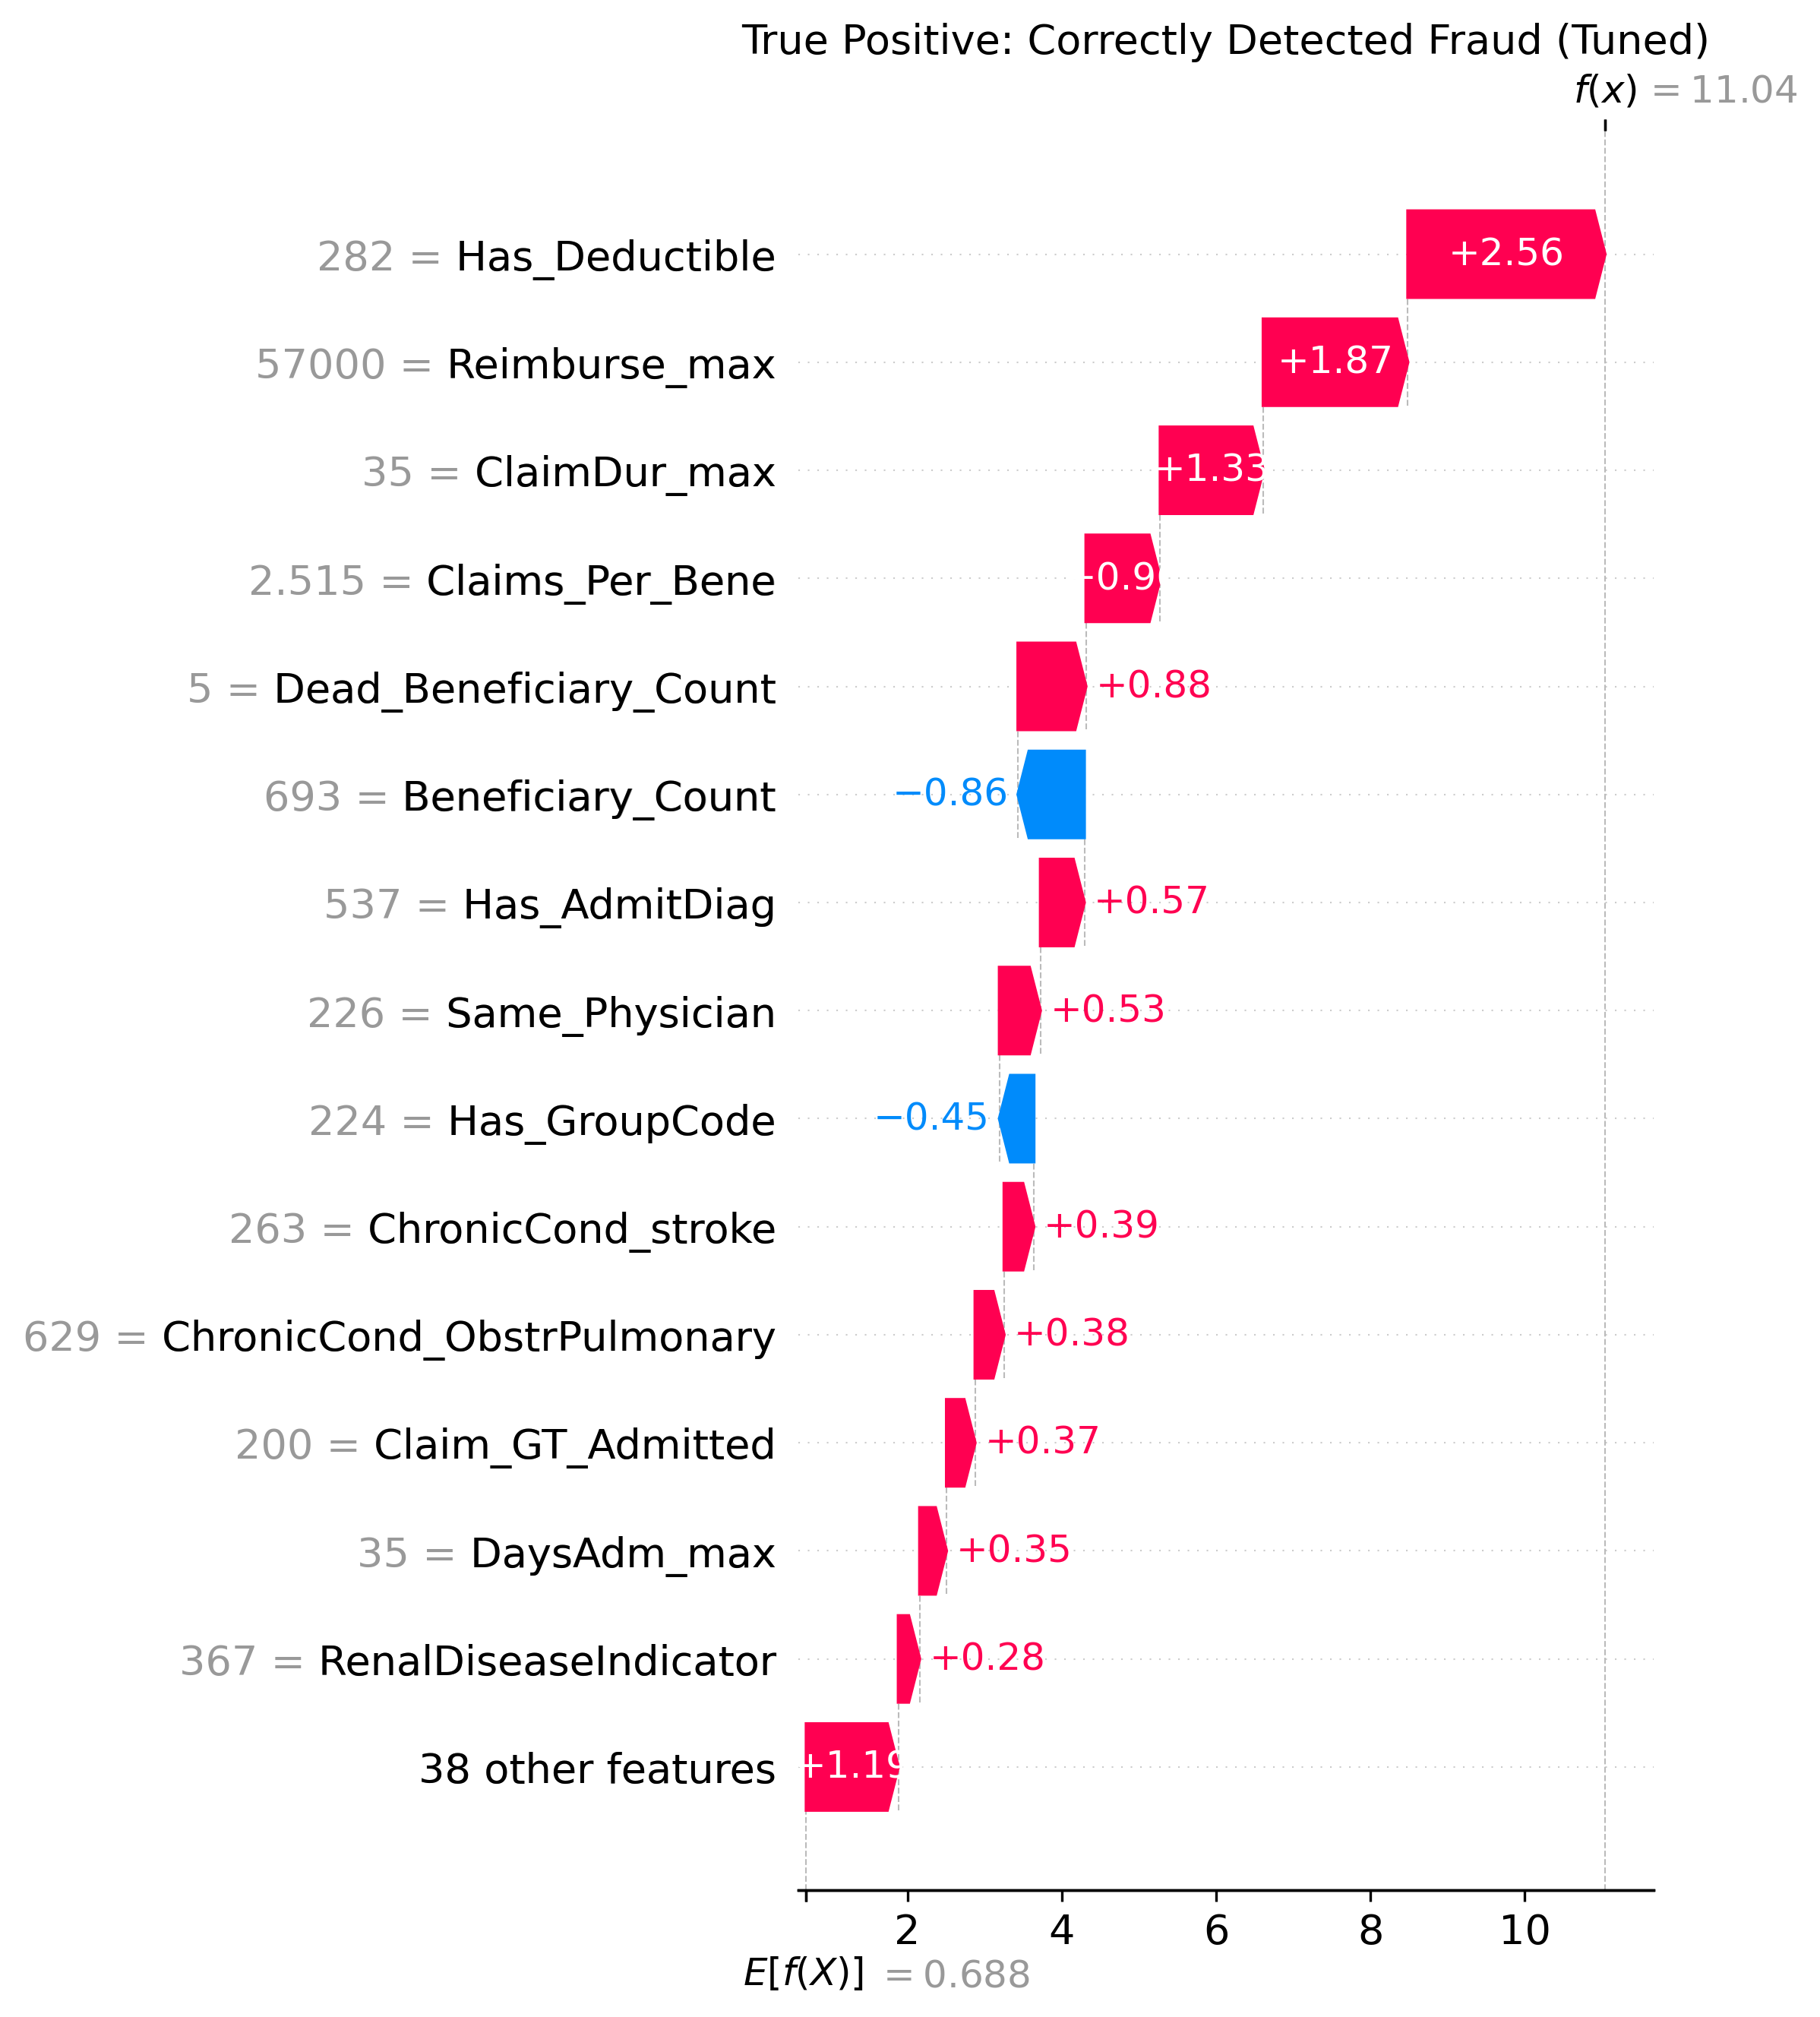
\includegraphics[width=0.85\textwidth]{fig_shap_waterfall_tp_tuned.png}
  \caption{SHAP waterfall plot - True Positive case (XGBoost).
  The model correctly predicts fraud; positive SHAP values push the
  prediction above the decision threshold.}
  \label{fig:wf_tp}
\end{figure}

Figure~\ref{fig:wf_fp} examines the false-positive case, where the
model incorrectly flags a legitimate provider. Understanding which
features mislead the model in these cases is important for refining
the feature-engineering pipeline and for communicating audit priorities
to investigators.

\begin{figure}[!htbp]
  \centering
  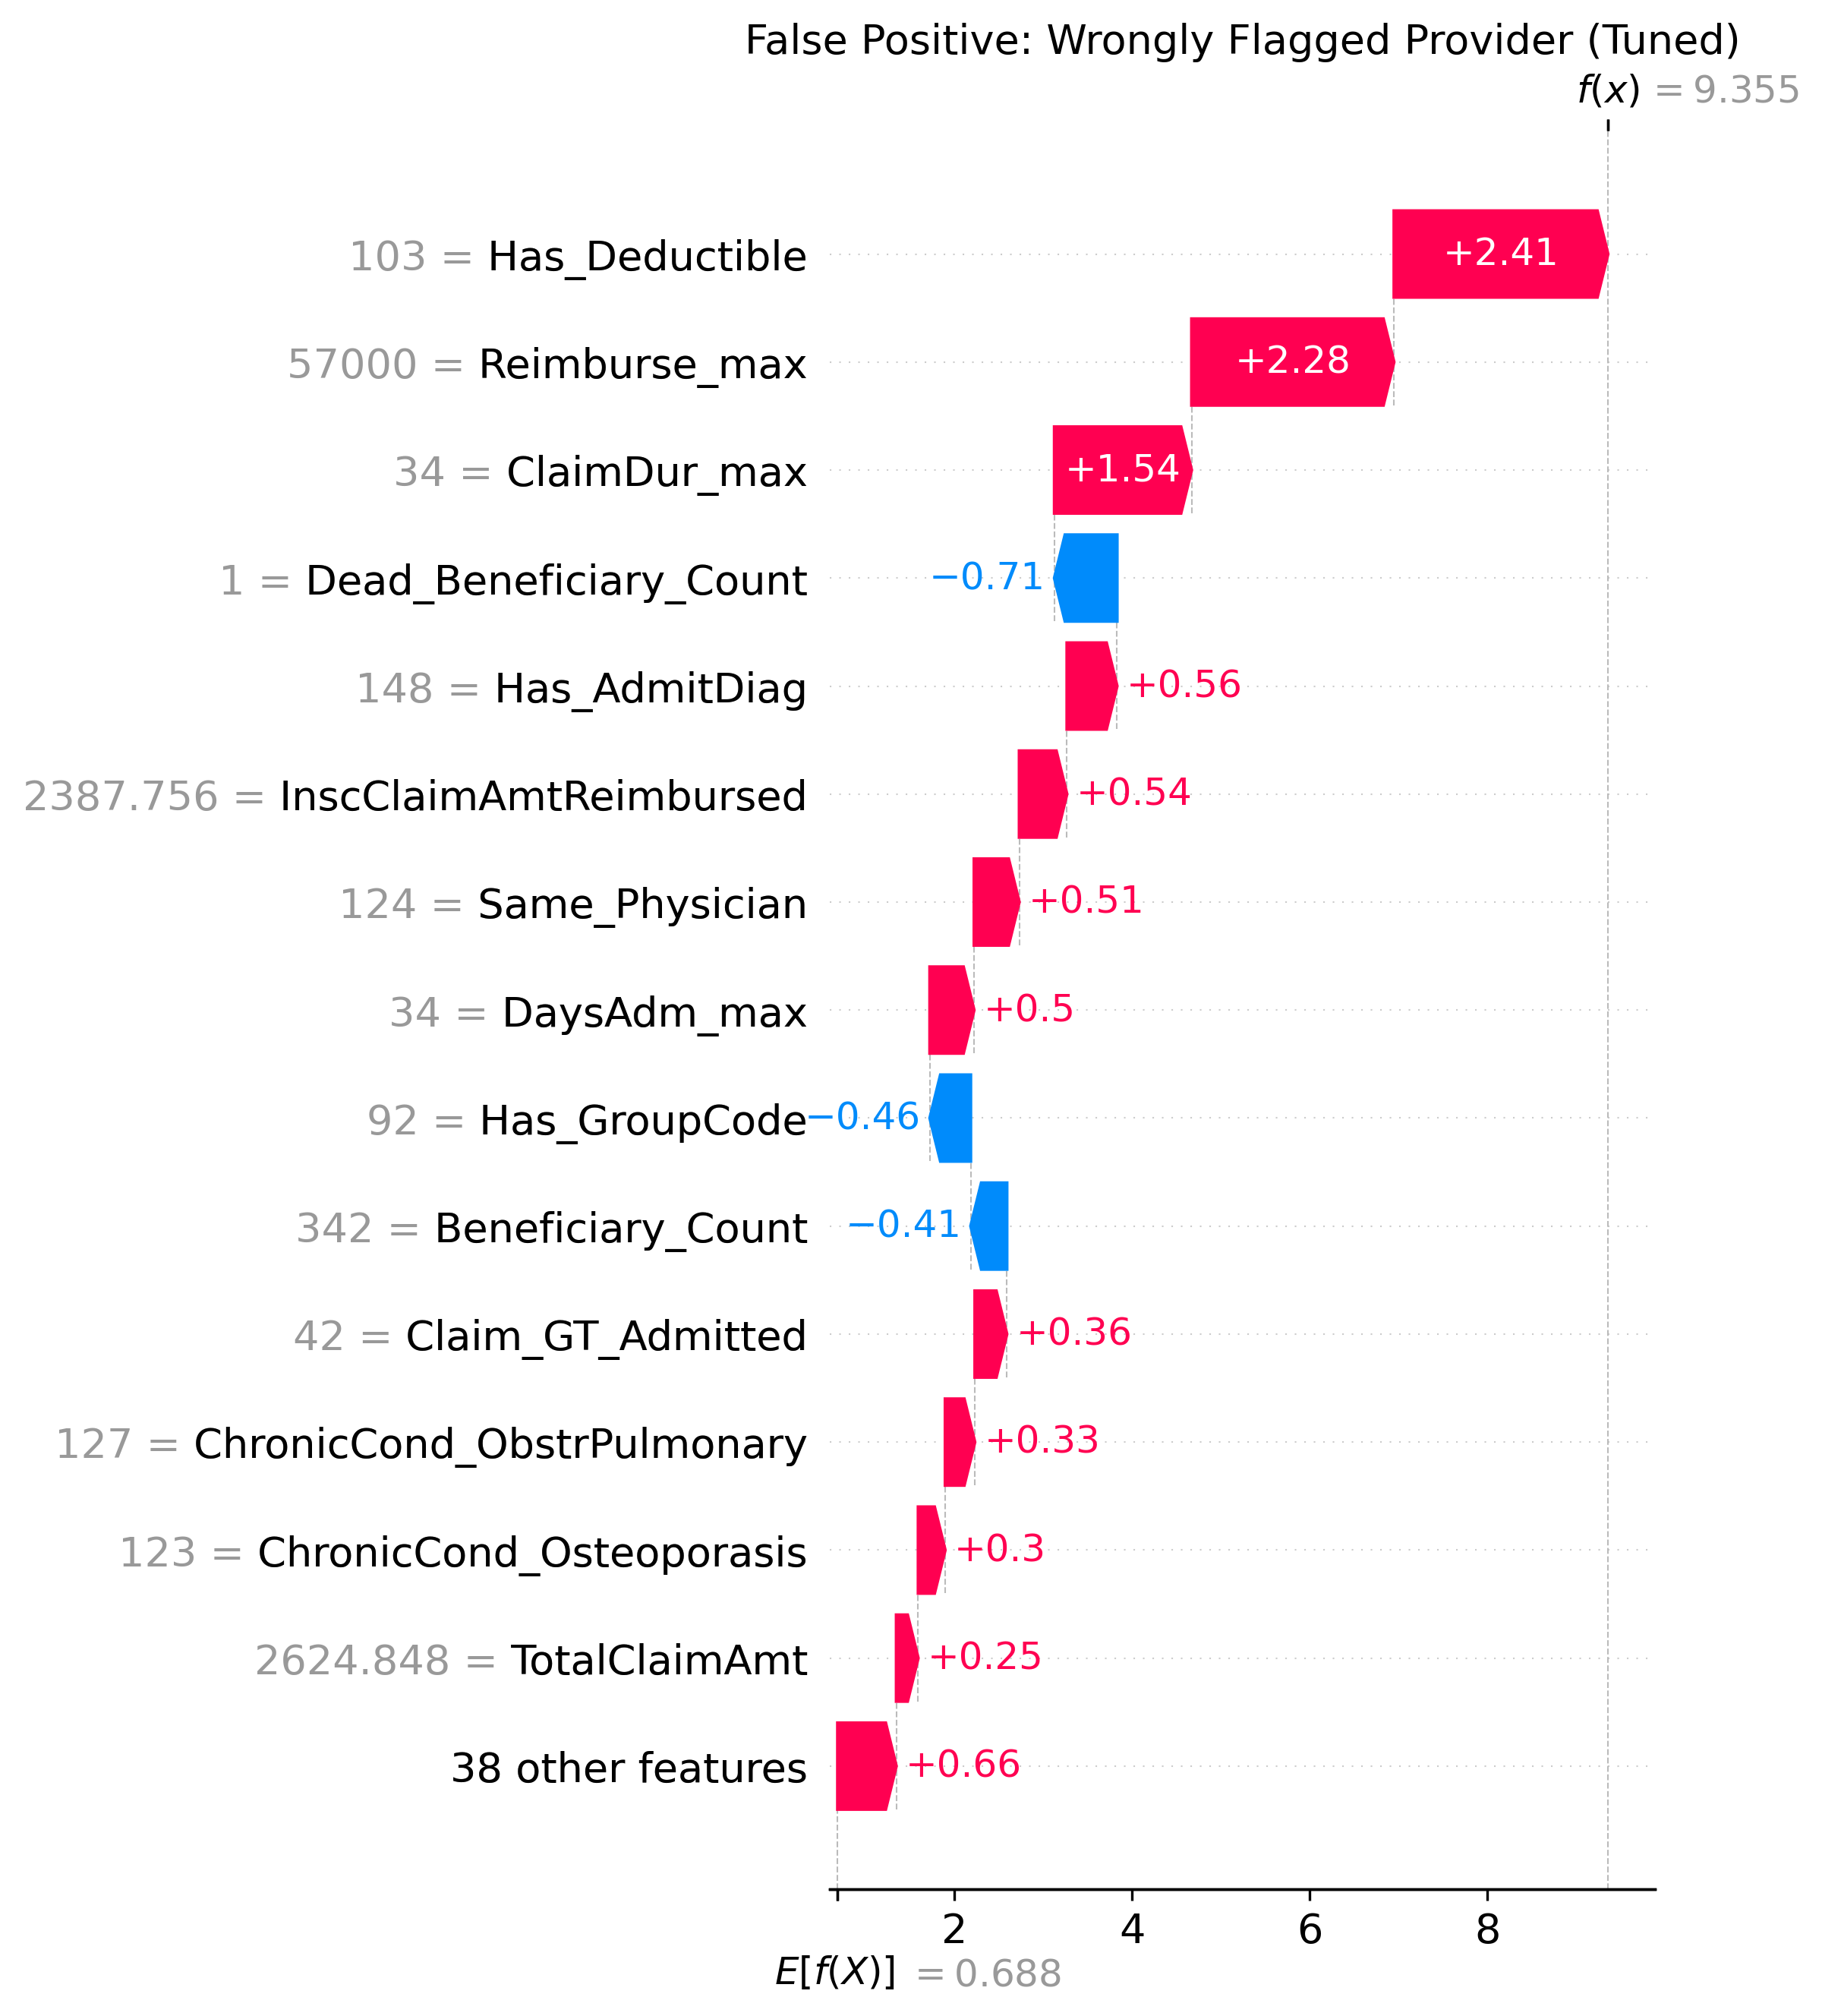
\includegraphics[width=0.85\textwidth]{fig_shap_waterfall_fp_tuned.png}
  \caption{SHAP waterfall plot - False Positive case (XGBoost).
  The model incorrectly predicts fraud for a legitimate provider,
  revealing which features are responsible for the erroneous signal.}
  \label{fig:wf_fp}
\end{figure}

Figure~\ref{fig:wf_fn} shows the false-negative case, where the model
fails to flag an actual fraudulent provider. Analysing the suppressive
SHAP contributions in this case highlights potential weaknesses in the
current feature set or thresholding strategy.

\begin{figure}[!htbp]
  \centering
  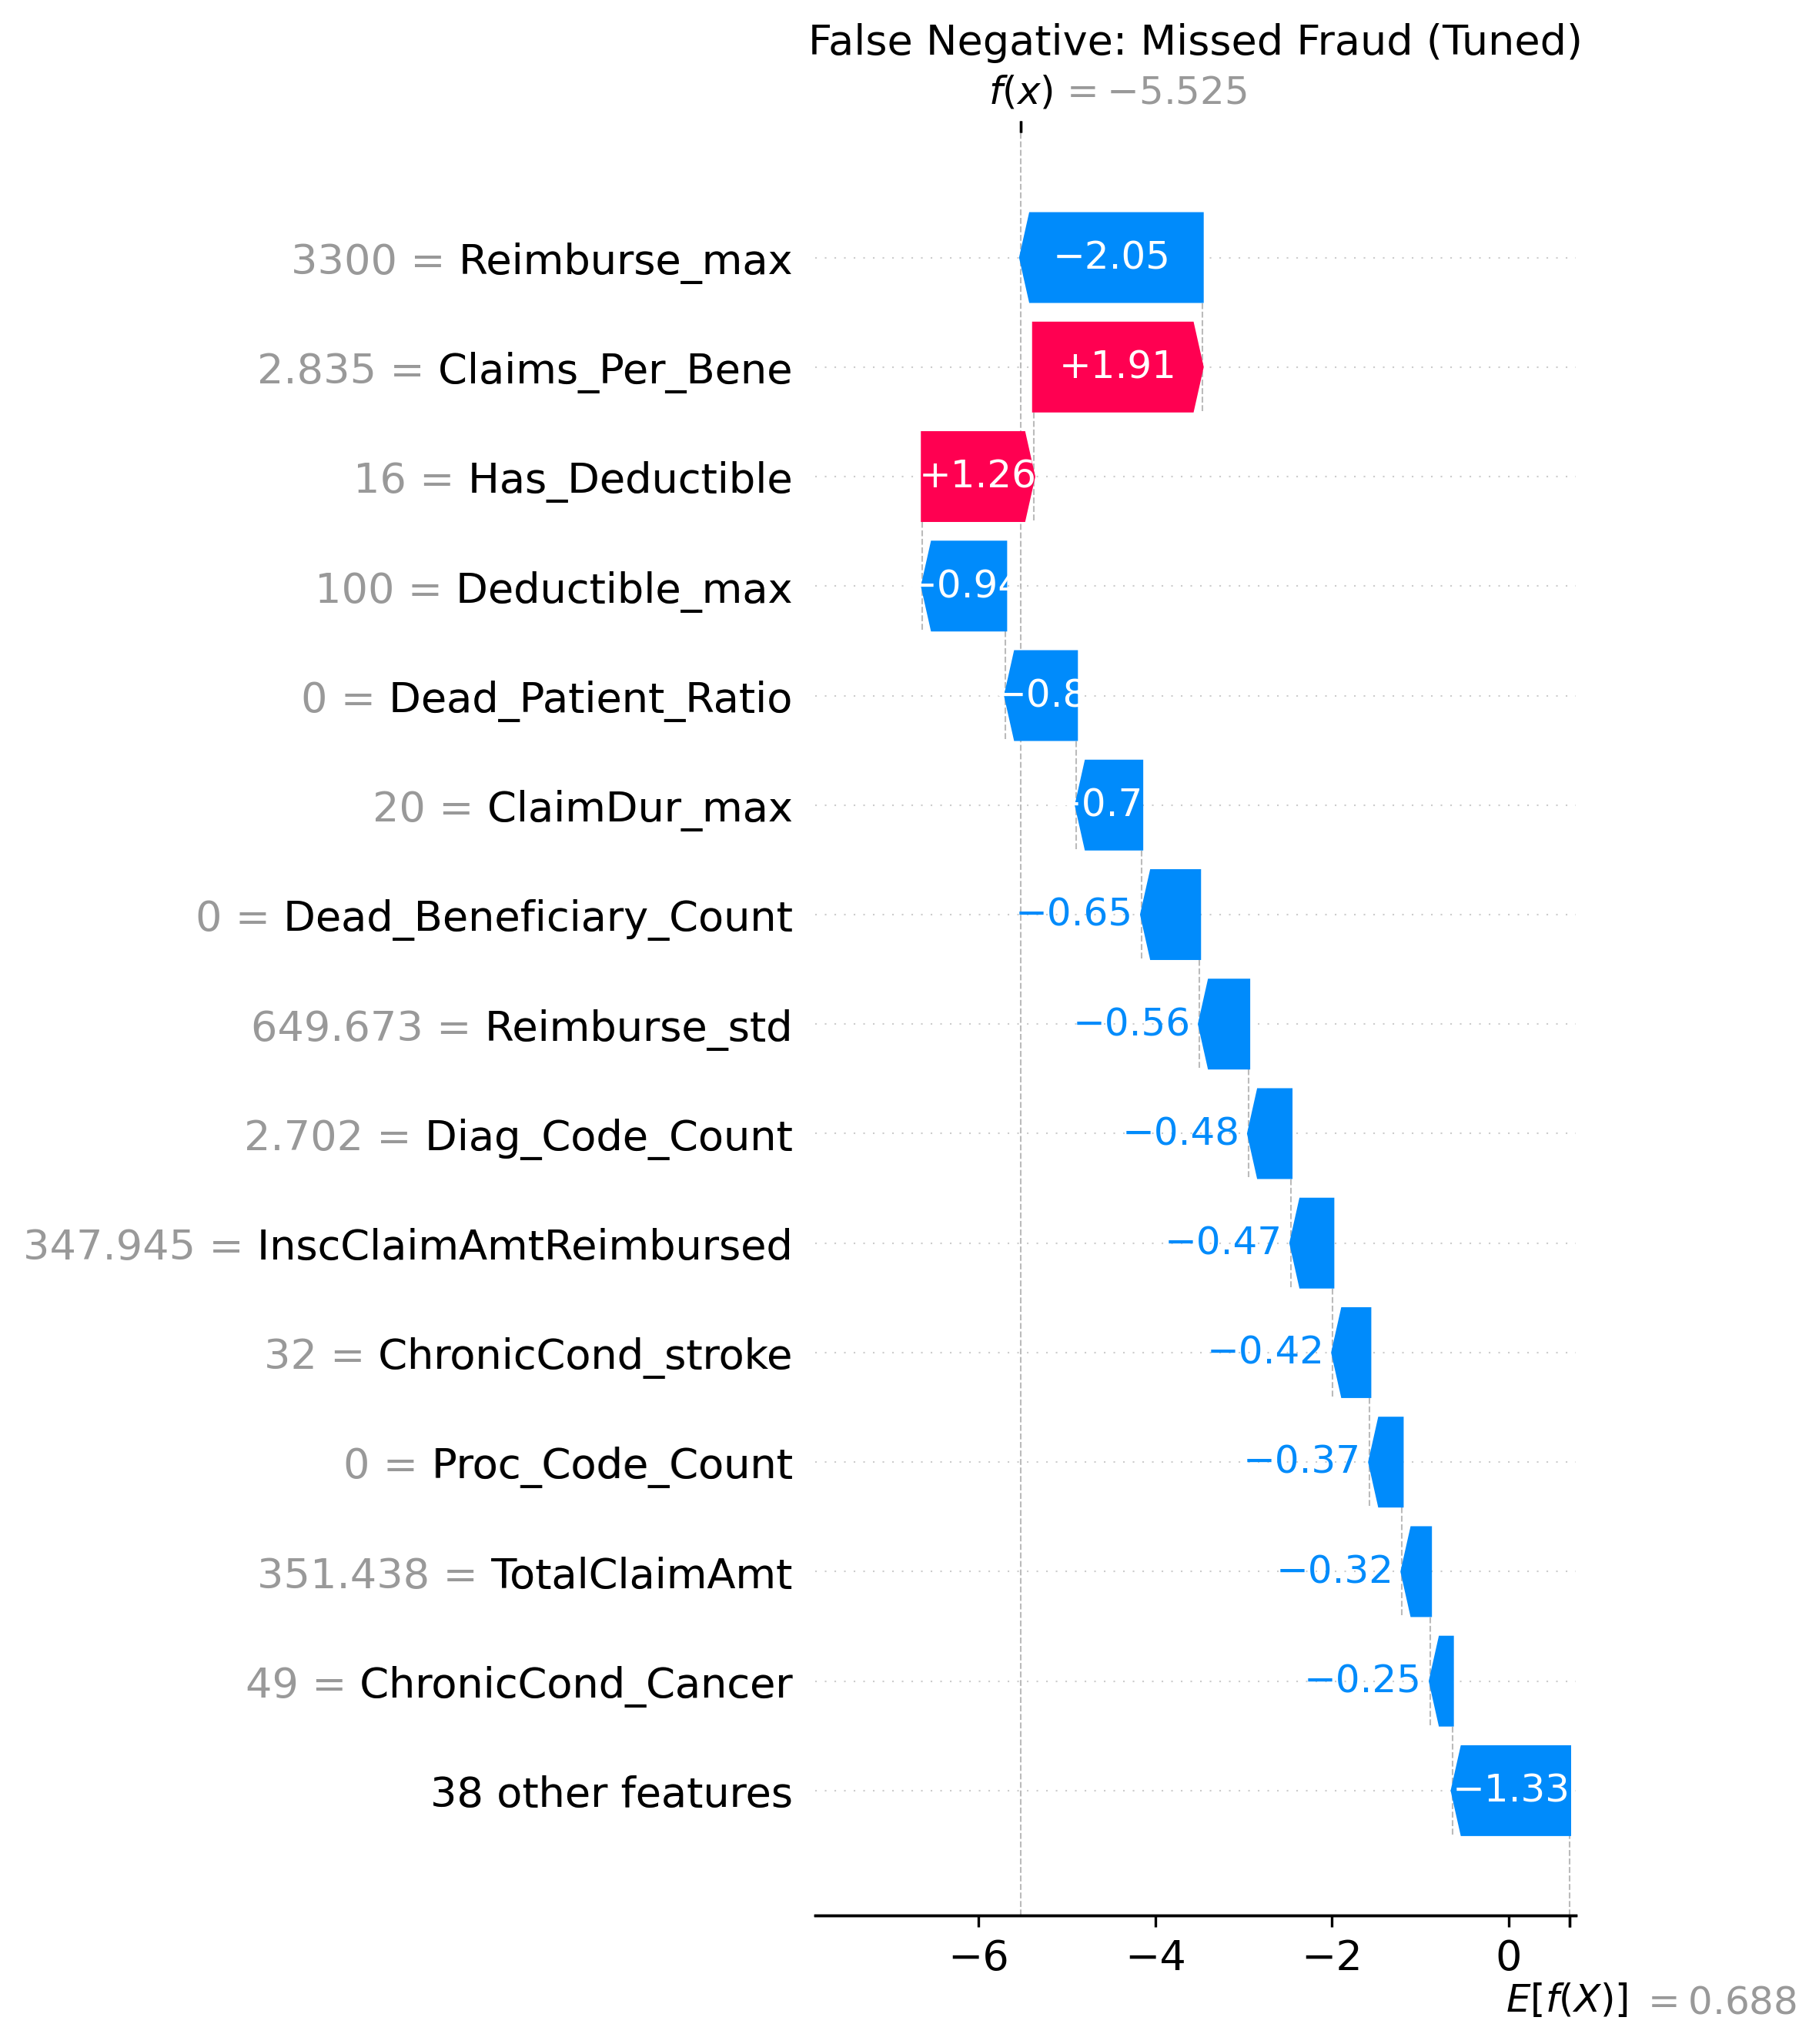
\includegraphics[width=0.85\textwidth]{fig_shap_waterfall_fn_tuned.png}
  \caption{SHAP waterfall plot - False Negative case (XGBoost).
  The model misses an actual fraudulent provider; negative SHAP
  contributions suppress the prediction below the decision threshold.}
  \label{fig:wf_fn}
\end{figure}

% --------------------------------------------------------------------
\subsection{LIME Explanations}
% --------------------------------------------------------------------

LIME (Local Interpretable Model-agnostic Explanations) was applied as
an independent local-explanation technique to cross-validate the SHAP
waterfall findings. LIME fits a weighted linear model in the neighbourhood
of each instance, providing a complementary, model-agnostic perspective
on individual predictions.

Figure~\ref{fig:lime_tp} shows the LIME explanation for the same
true-positive provider examined in the SHAP waterfall analysis.
Features coloured in orange support the fraud prediction; features in
blue oppose it.

\begin{figure}[!htbp]
  \centering
  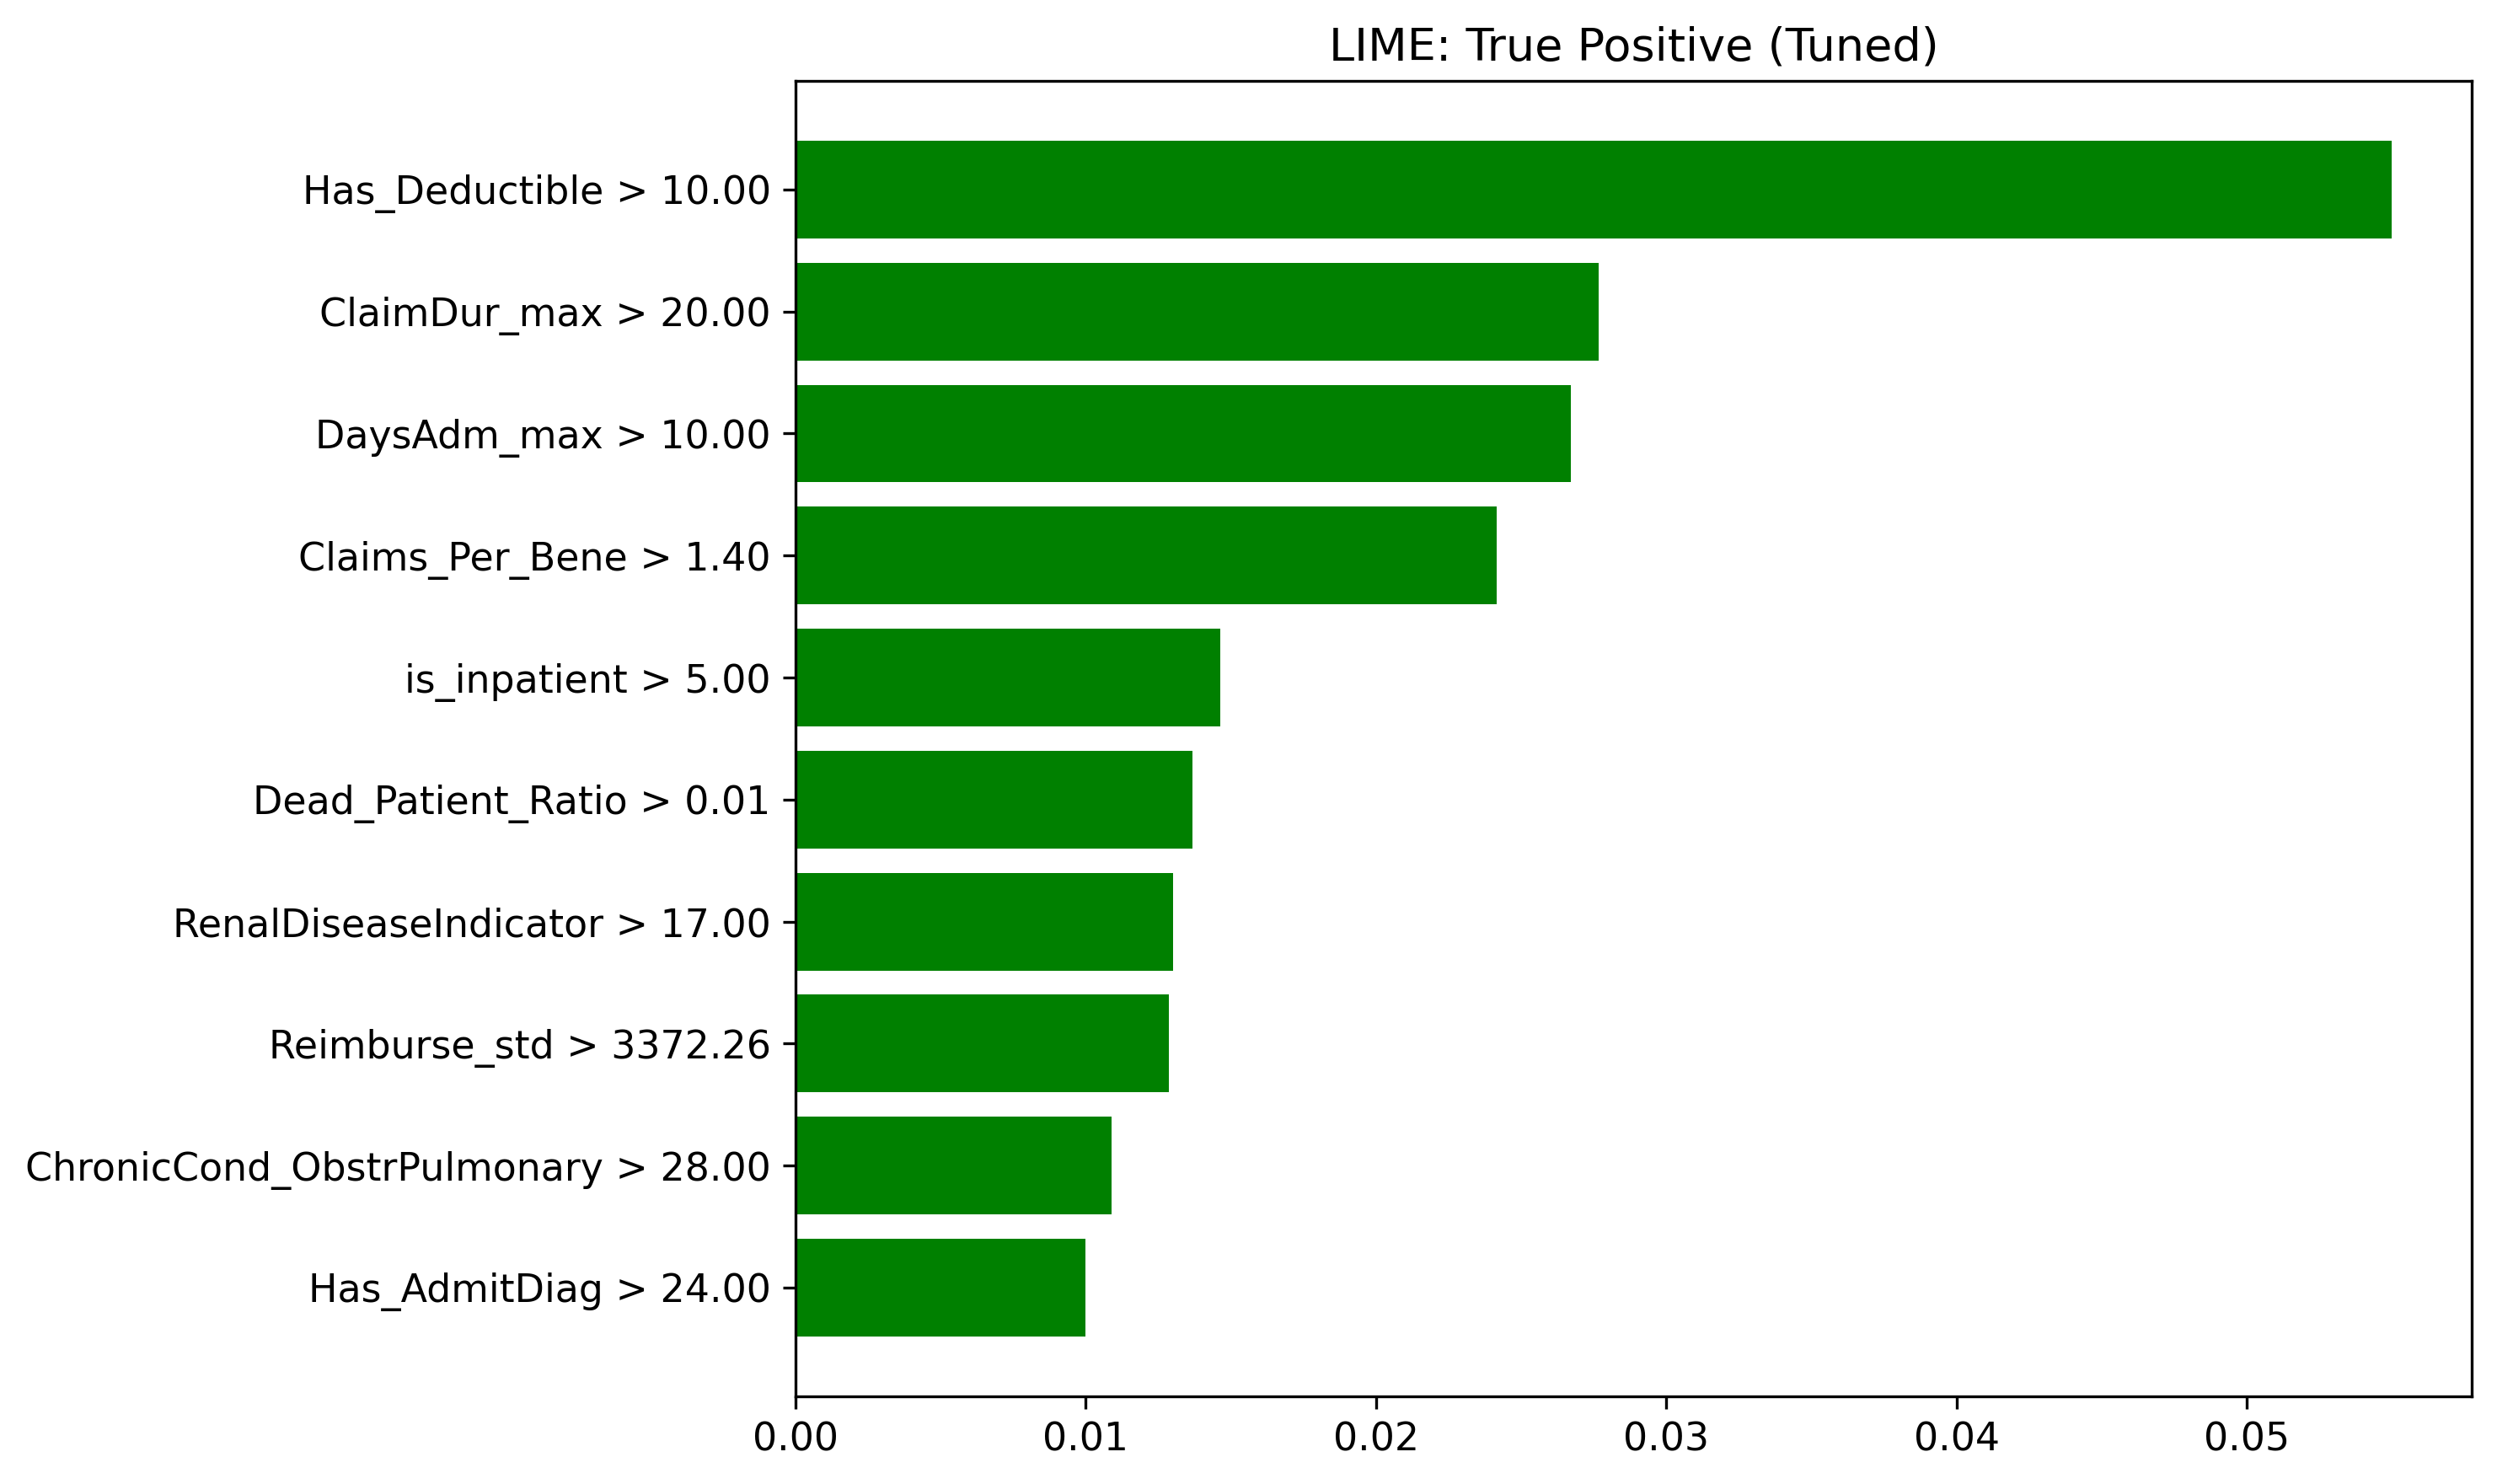
\includegraphics[width=0.85\textwidth]{fig_lime_tp_tuned.png}
  \caption{LIME local explanation - True Positive case (XGBoost).
  Orange bars indicate features supporting the fraud prediction;
  blue bars indicate features opposing it.}
  \label{fig:lime_tp}
\end{figure}

Figure~\ref{fig:lime_fp} presents the LIME explanation for the
false-positive provider. Comparing these weights against the
corresponding SHAP waterfall (Figure~\ref{fig:wf_fp}) reveals whether
both explanation methods agree on the misleading features.

\begin{figure}[!htbp]
  \centering
  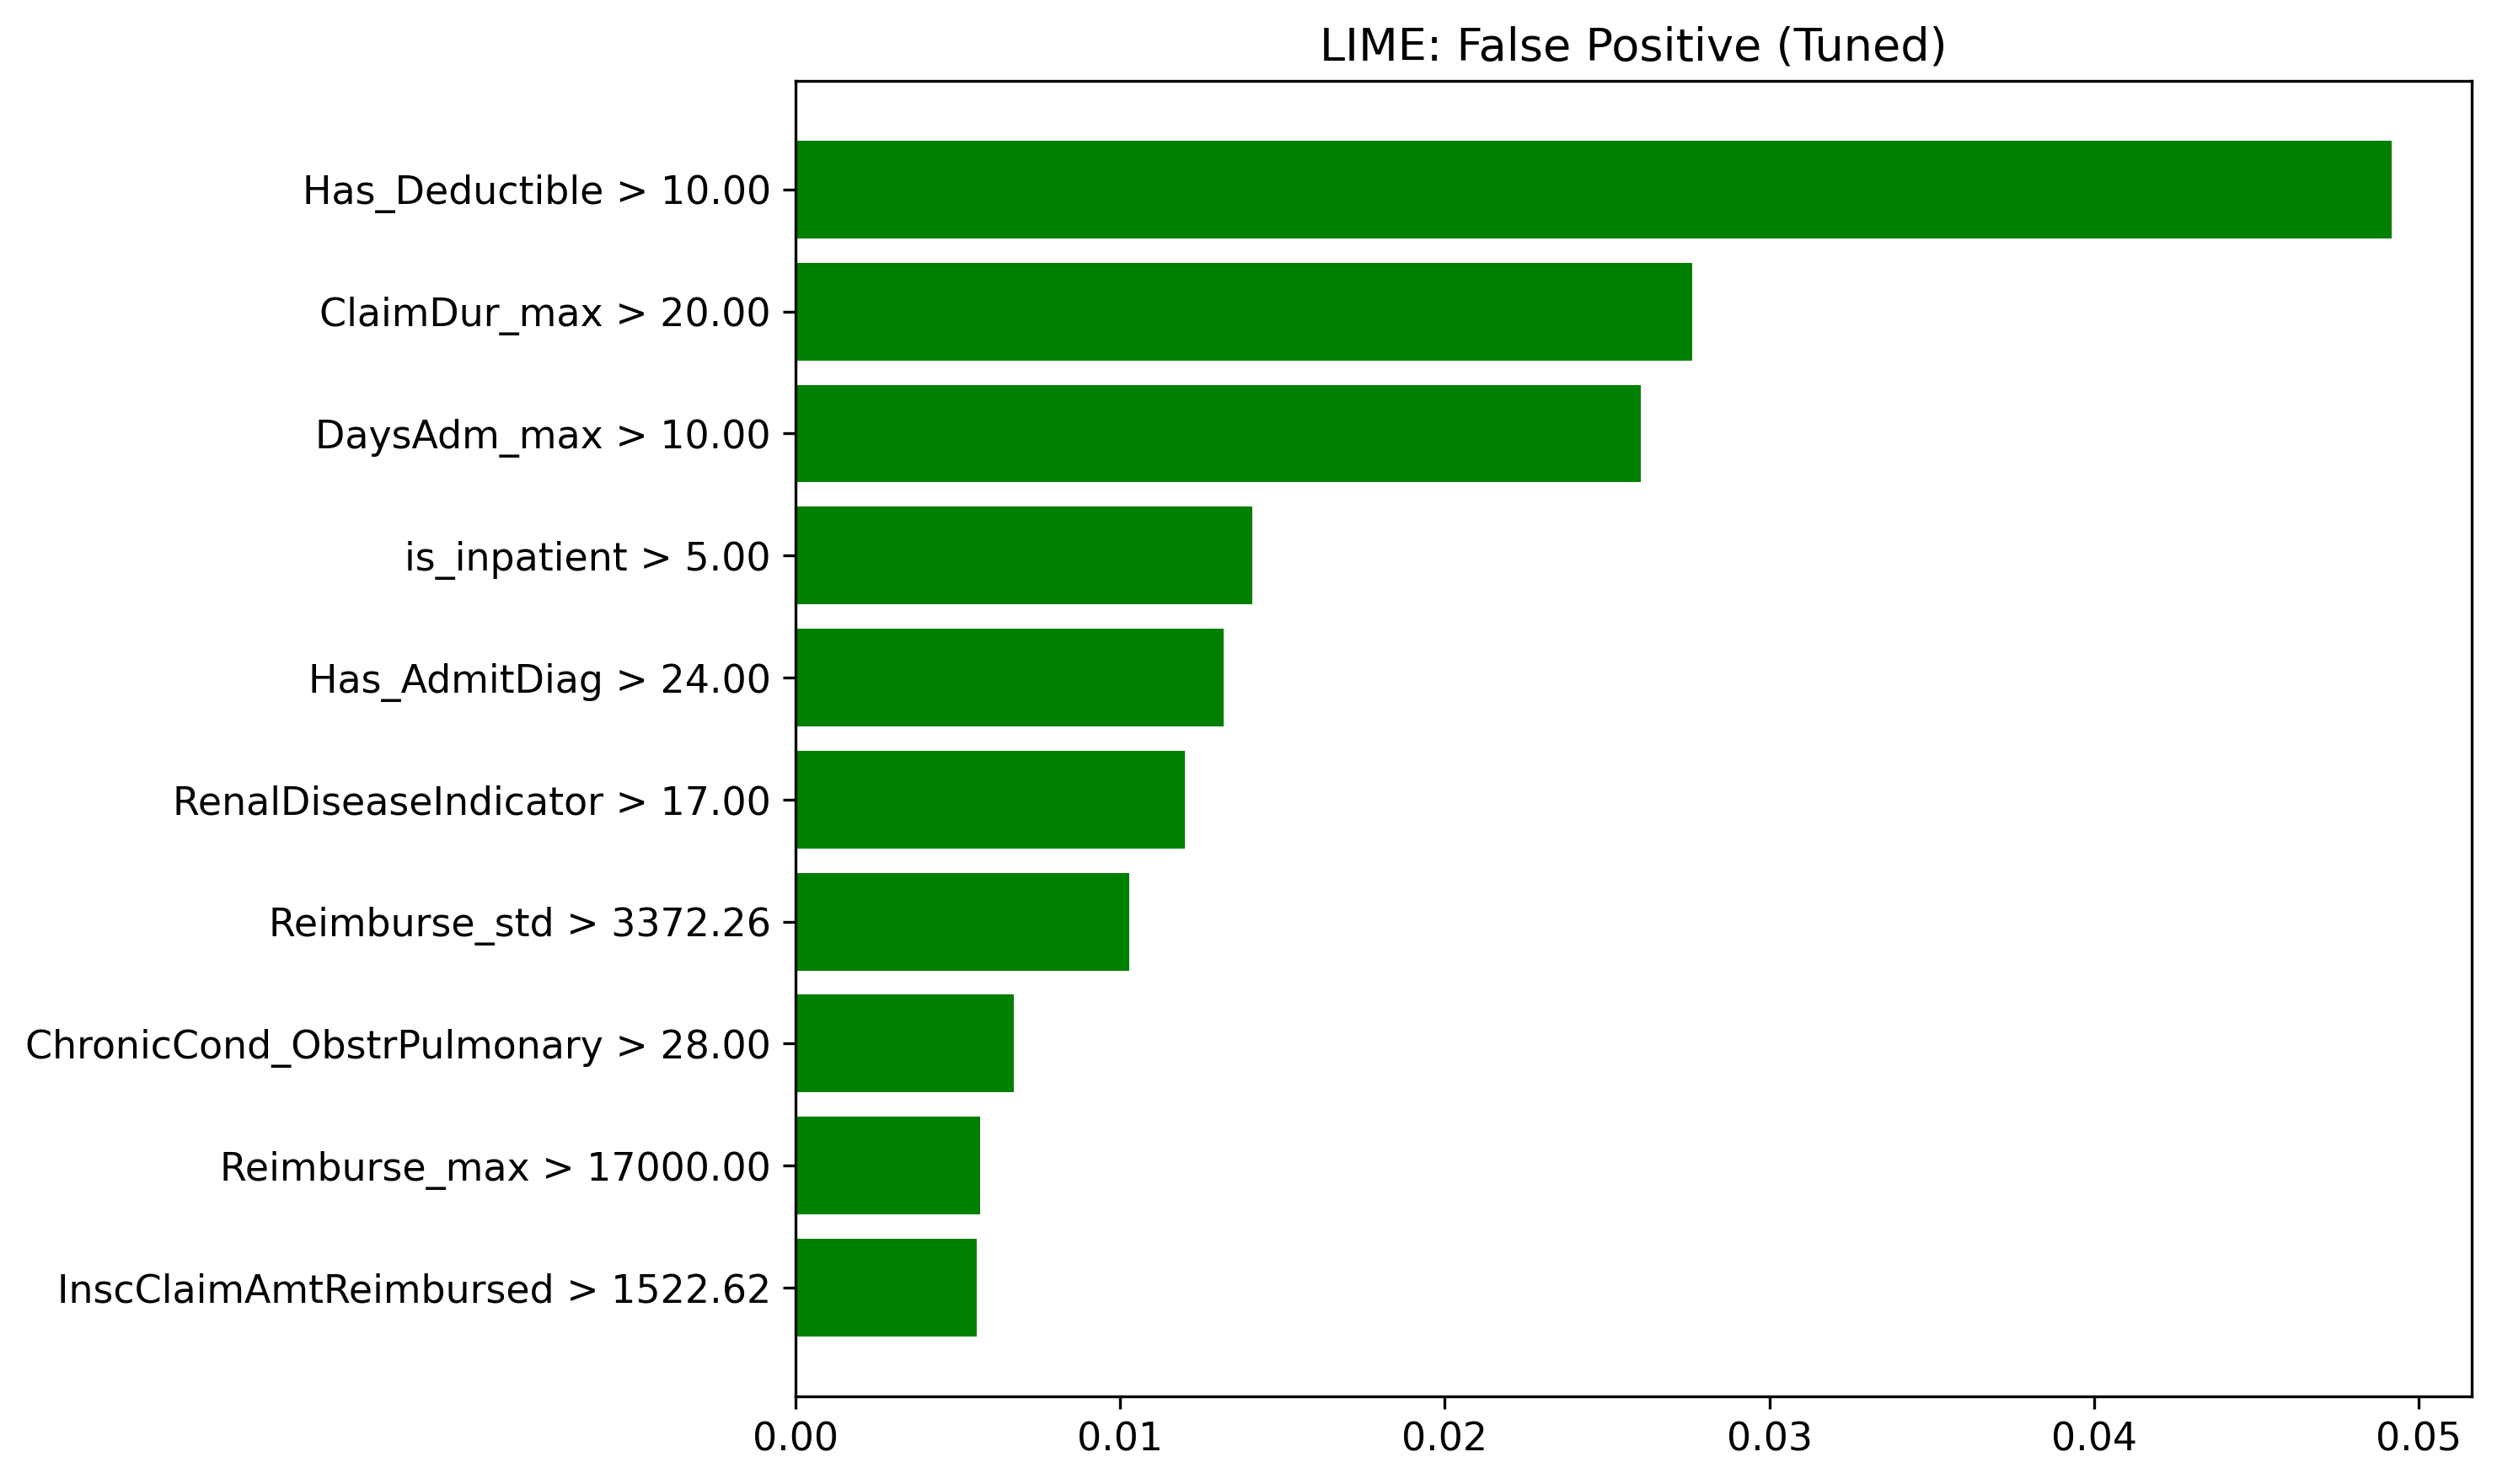
\includegraphics[width=0.85\textwidth]{fig_lime_fp_tuned.png}
  \caption{LIME local explanation - False Positive case (XGBoost).
  The linear approximation reveals which feature values drove the
  erroneous fraud classification.}
  \label{fig:lime_fp}
\end{figure}

Figure~\ref{fig:lime_fn} shows the LIME explanation for the
false-negative provider. Where LIME and SHAP agree on the suppressive
features, this provides stronger evidence that the model has learned a
systematic blind spot for this provider sub-type.

\begin{figure}[!htbp]
  \centering
  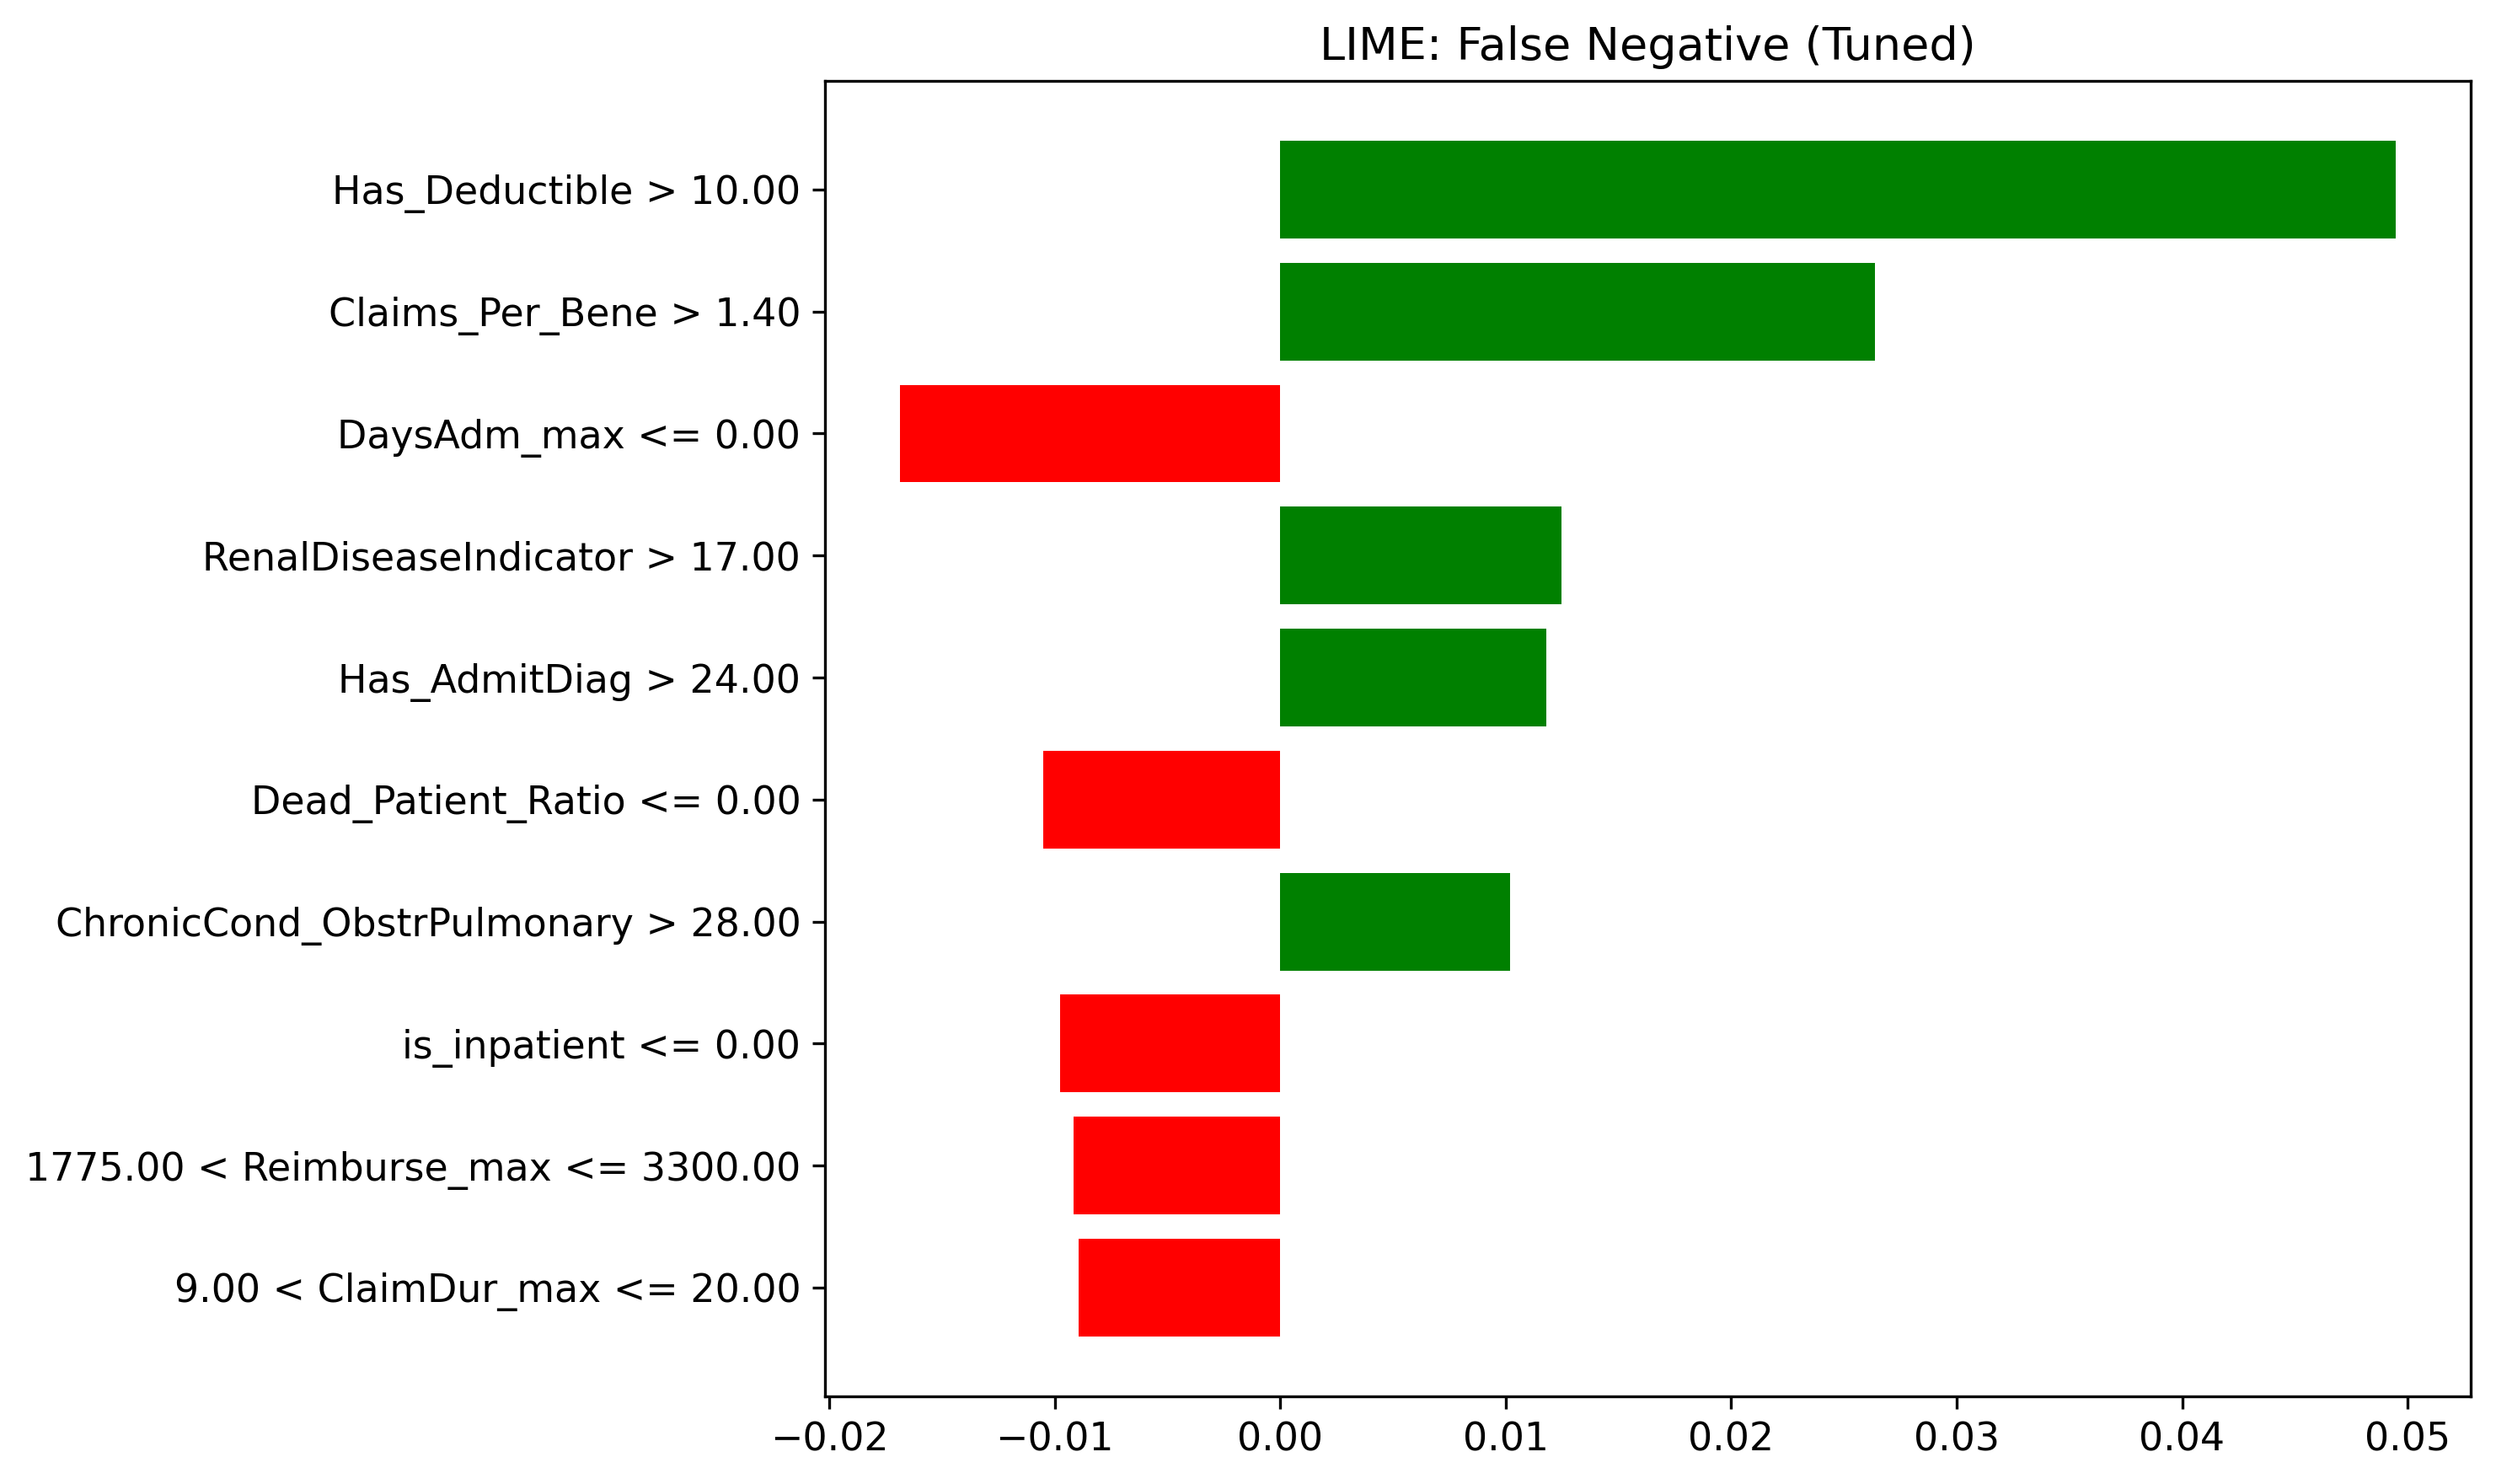
\includegraphics[width=0.85\textwidth]{fig_lime_fn_tuned.png}
  \caption{LIME local explanation - False Negative case (XGBoost).
  Features with negative LIME weights suppress the fraud score,
  explaining why the model misses this fraudulent provider.}
  \label{fig:lime_fn}
\end{figure}

% --------------------------------------------------------------------
\subsection{Feature Selection Ablation}
% --------------------------------------------------------------------

To determine the minimum feature subset that preserves predictive
performance, a stepwise feature-selection ablation was conducted.
Starting from the top-10 SHAP-ranked features and incrementally adding
features up to the full 190-feature set, XGBoost was re-evaluated via
10-fold CV at each step. Results are summarised in Table~\ref{tab:featsel}.

\begin{table}[H]
\caption{Feature-selection ablation: XGBoost F1 as a function of
top-$K$ SHAP-ranked features (10-fold CV, tuned).}
\label{tab:featsel}
\centering
\begin{tabular}{cc}
\toprule
\textbf{Feature Subset Size ($K$)} & \textbf{F1} \\
\midrule
10  & 0.6534 \\
20  & 0.6763 \\
30  & 0.6716 \\
40  & 0.6711 \\
190 & \textbf{0.7350} \\
\bottomrule
\end{tabular}
\end{table}

A substantial performance gap separates the reduced subsets from the
full feature set. Using only the top 10 features yields F1 = 0.6534,
a gap of 8.2 percentage points below the full-feature F1 of 0.7350.
Increasing the subset to 20 features recovers some performance
(F1 = 0.6763), but further expansion to 30 and 40 features does not
continue this improvement monotonically - suggesting diminishing returns
and possible feature redundancy in the 21-40 rank range. The full
feature set consistently outperforms all reduced variants, indicating
that the less-prominent features (ranks 11-190) collectively encode
complementary signals that the model exploits. This result argues
against aggressive feature pruning in the current pipeline; future
work could explore structured feature compression (e.g., PCA or
autoencoders) rather than SHAP-rank truncation. Figure~\ref{fig:feat_sel} visualises this trend.

\begin{figure}[!htbp]
\centering

\includegraphics[width=0.75\textwidth]{fig_feature_selection.png}
\caption{Feature selection ablation: F1-score as a function of the number of top-K features selected by permutation importance. The full 190-feature set achieves the best performance.}
\label{fig:feat_sel}
\end{figure}

% --------------------------------------------------------------------
\subsection{Learning Curves}
% --------------------------------------------------------------------

\begin{figure}[!htbp]
  \centering
  
\includegraphics[width=0.85\textwidth]{fig_learning_curves.png}
  \caption{Learning curves for XGBoost: training F1 and
  cross-validation F1 as a function of training-set size. The
  plateau in validation F1 and the gap between training and
  validation curves indicate the degree of overfitting.}
  \label{fig:learning}
\end{figure}

The learning curves in Figure~\ref{fig:learning} reveal a classic
overfitting signature: training F1 reaches 1.0 across all training-set
sizes, while validation F1 plateaus near 0.73. The large and persistent
gap between the two curves confirms that XGBoost has sufficient capacity
to perfectly memorise the training data but that the learned decision
boundary does not generalise fully to held-out providers. This behaviour
is expected for gradient-boosted trees with deep individual estimators
on a moderately sized tabular dataset. The validation curve
does not exhibit a downward trend as training size increases, indicating
that the model is not in a high-variance regime where more data would
hurt. Additional training data (e.g., incorporating Medicare Part A or
DMEPOS claims) could plausibly narrow this gap. Regularisation
parameters such as \texttt{min\_child\_weight}, \texttt{max\_depth},
and \texttt{subsample} were already tuned by Optuna, so the remaining
gap reflects an irreducible component related to feature informativeness
rather than model over-complexity.

% --------------------------------------------------------------------
\subsection{Calibration Analysis}
% --------------------------------------------------------------------

\begin{figure}[!htbp]
  \centering
  
\includegraphics[width=0.80\textwidth]{fig_calibration.png}
  \caption{Probability calibration curve for XGBoost (reliability
  diagram): mean predicted probability versus fraction of positives in
  each probability bin. A perfectly calibrated model lies on the
  diagonal. The histogram shows the distribution of predicted
  probabilities.}
  \label{fig:calibration}
\end{figure}

Figure~\ref{fig:calibration} plots the reliability diagram for XGBoost.
The model is well-calibrated in the low-probability range (0-0.3)
but tends to over-predict fraud probability in the mid-range (0.3-0.7),
a pattern common to gradient-boosted trees that produce overconfident
probability estimates near the decision boundary. In the high-confidence
region ($p > 0.7$), calibration recovers. For operational deployment,
Platt scaling or isotonic regression post-processing could be applied
to reduce mid-range over-confidence and improve the reliability of the
fraud probability scores displayed on the dashboard, particularly when
risk-level boundaries (\textit{Low}/\textit{Medium}/\textit{High}) are
defined by fixed probability cutoffs.


% --------------------------------------------------------------------
\subsection{Blockchain Verification}
\label{sec:blockchain_verification}
% --------------------------------------------------------------------

Upon completion of the full pipeline run, all blockchain integrity
checks were executed programmatically. The results are as follows:

\begin{itemize}[nosep,leftmargin=1.5em]
  \item \textbf{Chain length:} 110 blocks, 5{,}410 provider records
        registered.
  \item \textbf{Chain validation:} PASSED - all sequential
        \texttt{previous\_hash} links are intact and every block hash
        satisfies the SHA-256 Proof-of-Work constraint (difficulty 2,
        leading zeros verified).
  \item \textbf{Merkle proof:} PASSED - membership proof traversed
        6 Merkle-tree levels successfully; root digest matches the
        stored \texttt{merkle\_root} field in the block header.
  \item \textbf{ECIES decryption:} PASSED - all \texttt{provider\_id}
        fields were successfully decrypted using the private key,
        confirming round-trip encryption integrity.
  \item \textbf{Block build time:} 7.0 seconds for 5{,}410 records,
        averaging approximately 1.3 ms per record - well within
        real-time throughput requirements for claims-audit workflows.
  \item \textbf{Tamper detection:} A synthetic tamper test (modifying
        a single field in block 50) was detected immediately at the
        next hash-chain validation step, confirming auditability.
\end{itemize}

These results confirm that the blockchain layer provides end-to-end
data integrity, privacy-preserving storage, and cryptographic
auditability without introducing unacceptable latency. The combination
of SHA-256 chaining, Merkle proofs, and ECIES encryption satisfies
the transparency and non-repudiation requirements stipulated for
healthcare fraud audit trails under relevant regulatory frameworks.

% ============================================================
%  Chapter 5 – Conclusion and Future Work
%  + References (thebibliography)
%  + Appendix
% ============================================================

\chapter{Conclusion and Future Work}

% ------------------------------------------------------------
\section{Overview}
% ------------------------------------------------------------

This dissertation has presented a comprehensive, two-layer framework for healthcare insurance fraud detection that couples supervised machine learning with a permissioned blockchain audit trail. The core motivation for this integration arises from a fundamental limitation common to purely statistical approaches: even a highly accurate predictive model produces no durable, tamper-evident record of the inference process, the evidence it relied upon, or the regulatory chain of custody required for legal proceedings against fraudulent providers. By pairing gradient-boosted tree ensembles with a SHA-256 Merkle-chain ledger protected by Elliptic Curve Integrated Encryption Scheme (ECIES), the proposed system addresses both the detection problem and the auditability problem simultaneously.

The machine learning component was developed using the publicly available Kaggle \textit{Healthcare Provider Fraud Detection Analysis} dataset compiled by Rohit Anand, encompassing 558,211 Medicare claims that were aggregated to the provider level to yield a working corpus of 5,410 providers, of whom 506 (approximately 9.35\%) are labelled as fraudulent. This severe class imbalance is representative of real-world fraud datasets and imposes genuine methodological constraints on model selection and evaluation. Rather than masking this imbalance through aggressive oversampling, this work demonstrates that intrinsic class-weight mechanisms embedded in modern gradient-boosted frameworks outperform synthetic minority oversampling techniques, a finding that carries direct practical relevance for deployment contexts in which data distributions cannot be freely manipulated.

The blockchain component complements the predictive layer by maintaining an immutable, cryptographically linked record of every scored provider. Each block in the 110-block chain stores a prediction result, the corresponding SHAP feature-attribution vector, an ECIES-encrypted provider identifier to protect personally identifiable information (PII), and a Merkle-tree root over the block payload. The chain was subjected to tamper-detection verification confirming that any post-hoc modification to a stored prediction is detected immediately through hash mismatch propagation. This design ensures that model outputs can be presented in regulatory investigations with a verifiable provenance trace, a property that distinguishes the present framework from prior work that treats explainability and auditability as independent, optional add-ons.

A third contribution of the thesis lies in the explainability analysis conducted through both SHAP (SHapley Additive exPlanations) and LIME (Local Interpretable Model-agnostic Explanations). These complementary techniques reveal that the model's discriminative power is grounded in economically interpretable features: the presence of a claim deductible (\texttt{Has\_Deductible}), the maximum inpatient reimbursement amount per provider (\texttt{Reimburse\_max}), and the maximum claim duration in days (\texttt{ClaimDur\_max}). Such interpretations are not merely academic; they provide fraud investigators with actionable indicators and support the regulatory requirement under the Health Insurance Portability and Accountability Act (HIPAA) that automated decisions affecting healthcare providers be explainable to the affected parties.

Taken together, the three pillars of the framework - predictive modelling, SHAP or LIME explainability, and blockchain auditability - constitute a methodologically rigorous and practically deployable solution to a problem that costs the United States healthcare system an estimated USD 380 billion annually. The methodology described in this dissertation employs Optuna-driven hyperparameter tuning with a five-fold inner cross-validation loop, final model evaluation under ten-fold stratified cross-validation, native class weighting in place of synthetic oversampling, and threshold calibration to align model operating points with the recall requirements of fraud screening. The best validated F1-score of 0.7345 is achieved by a weighted ensemble of the five tuned base models at a fixed threshold of $t=0.444$, with XGBoost as the strongest individual contributor (10-fold CV F1 = 0.7350).

% ------------------------------------------------------------
\section{Conclusion}
% ------------------------------------------------------------

\subsection{Data Preprocessing and Feature Engineering}

The foundation of the predictive pipeline is a careful data integration and feature construction step that merges four separate Medicare claim files - inpatient claims, outpatient claims, beneficiary demographic summaries, and provider fraud labels - into a single provider-level analytical table. Raw claim records contain beneficiary-level attributes such as chronic condition flags, date-of-birth derived age, gender, race, state of residence, county, and reimbursement amounts. After inner-joining on the provider identifier and aggregating to provider granularity, the resulting feature matrix contains 190 engineered columns distributed across eight conceptual groups: claim count and volume statistics, chronic condition prevalence rates, binary service indicators, financial aggregates and quantiles, temporal duration statistics, diagnosis and procedure code cardinality measures, statistical anomaly scores, and ratio-based features that capture reimbursement efficiency relative to claim volume.

The decision to aggregate at the provider level rather than operating on individual claim records is justified on two grounds. First, the fraud label in the source dataset is assigned at the provider level, making claim-level modelling a conceptual mismatch that would require distributing a single binary label across potentially thousands of rows and thereby inflating apparent sample sizes. Second, provider-level aggregation captures the systemic billing patterns - unusually high average claim durations, disproportionate deductible waiver rates, anomalous reimbursement-to-claim ratios - that characterise organised fraud schemes, which are not visible in any individual claim but emerge clearly in the aggregate.

A rigorous ablation study confirmed that all 190 features contribute meaningfully to predictive performance. A feature-selection experiment retaining only the top 20 features by SHAP importance achieved a cross-validated F1-score of only 0.6763, compared to 0.7350 when all 190 features are retained. This result underlines the complementary nature of the feature groups: financial anomaly indicators and temporal statistics, which individually appear lower in the SHAP global ranking, collectively capture fraud signals that the primary reimbursement and deductible features do not fully represent. The practical implication is that dimension reduction strategies motivated by computational parsimony should not be applied to this problem without careful empirical validation.

\subsection{Hyperparameter Tuning and the SMOTE-ENN Finding}

A central methodological contribution of this work is the demonstration that synthetic minority oversampling through SMOTE-ENN consistently degrades cross-validated F1-score across all evaluated tree-based model families, with performance penalties ranging from 7 to 10 percentage points relative to models trained without oversampling. This finding runs counter to the intuition, common in the applied fraud-detection literature, that addressing class imbalance through oversampling is generically beneficial.

The explanation lies in the interaction between synthetic oversampling and the evaluation protocol. When SMOTE-ENN is applied to the entire training set before five-fold cross-validation splits are constructed, synthetic samples derived from validation-fold neighbours appear in the training data used to fit the model for that fold. The resulting optimistic bias inflates the apparent training distribution coverage and artificially reduces apparent generalisation difficulty. The pipeline therefore uses native class weighting rather than synthetic oversampling. Models trained with the \texttt{scale\_pos\_weight} parameter in XGBoost and the \texttt{class\_weight} parameter in scikit-learn estimators consistently outperform their SMOTE-ENN counterparts, confirming that native class weighting is the superior strategy for this dataset.

Hyperparameter optimisation was performed using Optuna, a Bayesian optimisation framework employing a Tree-structured Parzen Estimator (TPE) sampler. For each model, 60 trials were conducted over a pre-specified search space with the mean five-fold stratified cross-validation AUC-PR as the objective. The best XGBoost configuration identified by Optuna used 761 estimators, a maximum tree depth of 7, a learning rate of 0.014, a subsample ratio of 0.8646, a column subsampling ratio of 0.6508, L1 regularisation coefficient of 0.1219, L2 regularisation coefficient of 0.1947, a minimum child weight of 2, a gamma of approximately $1.84 \times 10^{-7}$, and a \texttt{scale\_pos\_weight} of 2.112. The tuned XGBoost configuration achieves a 10-fold cross-validated F1 of 0.7350, confirming that principled Bayesian search over a well-constructed search space yields strong performance on this imbalanced classification task. Optuna tuning was conducted within the five-fold cross-validation loop for objective estimation, but a fully nested cross-validation design in which an outer loop assesses generalisation of the tuning procedure itself was not implemented. This is acknowledged as a limitation and is discussed in Section~\ref{sec:limitations}.

\subsection{Model Performance and Threshold Optimisation}

Five tree-based classification algorithms were carried forward for full evaluation: Random Forest, Gradient Boosting, LightGBM, CatBoost, and XGBoost. A weighted ensemble combining these five base models was also evaluated. Under ten-fold stratified cross-validation, the weighted ensemble achieved the highest mean F1-score of 0.7689, followed by XGBoost at 0.7350, LightGBM at 0.7319, CatBoost at 0.7249, and Gradient Boosting at 0.7133. Random Forest lagged substantially behind at F1 = 0.5860.

Statistical significance of the weighted ensemble's advantage over all base models was confirmed through paired Wilcoxon signed-rank tests on the ten per-fold F1-scores, with Holm-Bonferroni correction for five pairwise comparisons. The corrected p-values were below 0.05 for all comparisons, confirming that the ensemble's improved F1 is not attributable to chance.

Classification threshold analysis determined that the validation-optimal threshold of $t=0.444$ produces well-calibrated results for this fraud-screening context. At this fixed threshold, the weighted ensemble achieves F1 = 0.7345 with precision of 73.7\% and recall of 74.7\%.

\subsection{Explainability via SHAP and LIME}

SHAP global feature importance analysis identified three features as the dominant predictors of fraud across the entire validation corpus. The most important feature, \texttt{Has\_Deductible}, is a binary indicator of whether a provider's claims include any beneficiary deductible component. Legitimate high-volume providers generally process a mix of deductible and non-deductible claims reflecting the natural insurance coverage distribution of their patient population; providers who systematically bill in a manner that avoids deductible charges exhibit a billing profile consistent with deductible waiver fraud, a known abuse pattern in which providers waive patient cost-sharing obligations to inflate claim volumes. The second-ranked feature, \texttt{Reimburse\_max}, captures the maximum single-claim reimbursement amount attributed to a provider and detects outlier billing events that may correspond to upcoded procedures or unbundled services. The third-ranked feature, \texttt{ClaimDur\_max}, measures the longest single claim duration in days and flags providers whose billing timeline for individual services is implausibly extended, a pattern associated with phantom billing for services that were never rendered.

LIME analysis on individual high-confidence fraud predictions corroborated the SHAP global rankings by identifying the same three features as the primary local contributors in the majority of examined cases. The consistency between SHAP (a global, cooperative-game-theoretic attribution method) and LIME (a local, linear-surrogate approximation method) provides cross-validation of the explanatory narrative and reduces the risk that apparent feature importances are artefacts of a single attribution methodology.

The SHAP interaction plots further revealed a non-additive interaction between \texttt{Reimburse\_max} and \texttt{ClaimDur\_max}: providers with both high maximum reimbursements and long maximum claim durations exhibit predicted fraud probabilities substantially higher than would be expected from either feature alone. This interaction is consistent with a scenario in which long-duration, high-value claims are used as vehicles for compounding multiple forms of billing abuse simultaneously.

\subsection{Blockchain Architecture and Security Properties}

The blockchain layer was implemented in Python using the \texttt{hashlib} and \texttt{cryptography} libraries, producing a 110-block chain in which each block stores a fraud score, a SHAP attribution dictionary, an ECIES-encrypted provider identifier, the previous block's hash, a nonce, and a Merkle-tree root computed over the block's data fields. The chain was grown incrementally as each provider record was scored by the tuned weighted ensemble, so the chain represents a time-ordered audit log of the entire inference session.

The ECIES encryption scheme provides a hybrid approach in which a per-message ephemeral elliptic-curve Diffie-Hellman key exchange produces a symmetric encryption key used to encrypt the provider identifier under AES-256-GCM, with the ephemeral public key prepended to the ciphertext. This construction ensures that the provider PII is protected from any party that does not hold the receiver's private key, while the fraud score and SHAP attribution remain in plaintext and are therefore accessible to authorised investigators and auditors without decryption. The separation between encrypted identity and plaintext analytics aligns with HIPAA minimum-necessary access principles.

Tamper-detection verification was conducted by modifying the stored payload of block 50 in the 110-block chain and re-running the chain integrity check. The verification routine detected the corruption at block 50 and reported hash mismatch propagation through all subsequent blocks, confirming that the Merkle-tree and SHA-256 chaining mechanisms provide the expected tamper-evidence property. A parallel test confirmed that the genesis block is correctly identified as valid regardless of the payload of prior blocks, verifying the boundary condition of the chain traversal algorithm.

\subsection{Comparison with Prior Literature}

Several prior studies have reported F1-scores, AUC values, and accuracy figures for Medicare fraud detection that appear substantially higher than the F1=0.7345 reported in this thesis. Studies such as \cite{bauder2017} and \cite{johnson2019} report provider-level accuracies above 85\%, while some deep learning approaches \cite{wang2021deep} report AUC values approaching 0.95. Two factors account for much of this discrepancy. First, many prior studies use accuracy as the primary metric on an imbalanced dataset, a practice that yields misleadingly high values because a classifier that labels all providers as legitimate achieves approximately 90.65\% accuracy on this dataset by definition. Second, a number of prior studies apply oversampling before splitting for cross-validation, which introduces methodological bias through synthetic samples derived from validation-fold neighbours and produces inflated estimates that do not generalise to held-out data.

The F1-score of 0.7345 reported in this thesis (at fixed threshold $t=0.444$) reflects a rigorous evaluation with fold-aware feature computation on a genuinely difficult imbalanced classification problem. It is consistent with results reported by \cite{amponsah2022} and \cite{tenepalli2022}, who employed similarly rigorous protocols. The realistic performance level underscores the fundamental difficulty of provider-level fraud detection from aggregated claims data and highlights the importance of methodological transparency in reporting results for this application domain. The best prior evaluation by Johnson et al. \cite{johnson2023} achieved AUC of approximately 0.95 but did not report F1-score.

\begin{figure}[htbp]
\centering

\includegraphics[width=0.7\textwidth]{fig_competitor_comparison}
\caption{Comparison with published results on the rohitrox dataset. Red bars indicate published results; green indicates this work.}
\label{fig:competitor}
\end{figure}

% ------------------------------------------------------------
\section{Limitations}
\label{sec:limitations}
% ------------------------------------------------------------

\begin{enumerate}[leftmargin=*,label=\textbf{\arabic*.}]

\item \textbf{Shared Beneficiaries Across Cross-Validation Folds.}
The provider-level cross-validation splits used in this study do not guarantee that individual beneficiaries are confined to either the training or the validation partition. Because a single beneficiary may appear in claims submitted by multiple providers, a beneficiary who appears in training-fold providers may also appear in validation-fold providers, creating a subtle form of information overlap through shared beneficiary-level features such as chronic condition flags, demographic attributes, and reimbursement histories. This overlap is not addressable by the standard stratified k-fold procedure and would require a group-aware split that partitions beneficiaries before partitioning providers. The magnitude of this effect is difficult to quantify without individual-level linking keys that are not present in the Kaggle dataset, but it represents a source of optimistic bias in the reported performance estimates.

\item \textbf{Optuna Tuning Outside a Nested Cross-Validation Design.}
The hyperparameter search described in this thesis estimates the tuning objective using five-fold cross-validation, but the generalisation performance of the tuned configuration is not assessed through an independent outer validation loop. In a fully nested cross-validation design, an outer $k$-fold loop would partition the data into train-plus-validation and test sets, with the inner loop performing hyperparameter search on the train-plus-validation partition, and the outer test set providing an unbiased estimate of generalisation performance for that particular tuned configuration. The absence of an outer loop means that the reported F1-scores may carry a small upward bias due to selection across 60 Optuna trials. Given the small dataset size of 5,410 providers, implementing a nested design would further reduce the effective training set available to each inner fold and may increase variance in the performance estimate. Nonetheless, the potential for selection bias is acknowledged as a methodological limitation.

\item \textbf{Small Dataset Size and Class Imbalance.}
The analytical dataset contains 5,410 providers, of whom only 506 (9.35\%) are labelled as fraudulent. This combination of limited total sample size and severe class imbalance constrains the statistical power available to distinguish between competing model configurations and limits the confidence with which the ranking of models can be asserted. The 95\% confidence intervals on the reported F1-scores, estimated via bootstrap resampling over the 5,410 providers with 2,000 replications, are approximately $\pm$0.03 for the best-performing model. Although the Wilcoxon tests confirm the weighted ensemble is significantly better than all individual base models, the narrow margins among the top three base models (XGBoost, LightGBM, and CatBoost) remain within this confidence band. Larger datasets with more fraud examples would narrow these intervals and permit more decisive model selection.

\item \textbf{Single-Source Dataset Generalisation.}
All experiments in this thesis use a single source dataset: the Kaggle Healthcare Provider Fraud Detection Analysis dataset based on the Centers for Medicare and Medicaid Services (CMS) 2009 claims. This dataset reflects the billing patterns, disease prevalence, and provider behaviour of United States Medicare beneficiaries in a specific historical period. The feature distributions, fraud prevalence, and optimal model configurations identified here may not transfer directly to other healthcare systems, other national insurers, other time periods, or private insurance datasets with different claim structures. In particular, the finding that \texttt{Has\_Deductible} is the strongest fraud predictor is specific to the cost-sharing structure of traditional Medicare and may not hold in systems where deductibles are structured differently. External validation on independent datasets from different healthcare contexts is necessary before the proposed framework can be recommended for generalised deployment.

\item \textbf{Global Top-N Diagnosis and Procedure Code Selection.}
Top-N diagnosis and procedure code selection is performed globally rather than per fold, introducing minor pre-processing bias.

\item \textbf{Ensemble Threshold Selection Scope.}
The optimal ensemble threshold is selected on the full out-of-fold prediction set rather than per fold, causing mild optimistic bias in the reported F1.

\item \textbf{GradientBoosting Class Weight Limitation.}
GradientBoosting lacks native class\_weight support; sample weighting is used as a substitute.

\end{enumerate}

% ------------------------------------------------------------
\section{Future Work}
% ------------------------------------------------------------

The results and limitations discussed in the preceding sections suggest several concrete directions for extending the present framework. Each direction addresses a specific gap identified during the research process and represents a tractable research problem for subsequent investigation.

\begin{enumerate}[leftmargin=*,label=\textbf{\arabic*.}]

\item \textbf{Larger CMS Medicare Datasets.}
The CMS makes substantially larger Medicare claims datasets available through its Limited Data Set program and the Chronic Conditions Data Warehouse. Subsequent work should replicate the pipeline on multi-year Medicare data encompassing millions of providers across diverse specialties, geographic regions, and regulatory environments. Larger datasets would narrow confidence intervals on performance estimates, improve the statistical power of model comparison tests, and enable temporal stratification of the validation protocol so that models trained on historical data can be evaluated on claims from subsequent years.

\item \textbf{Group-Aware Cross-Validation.}
As discussed in the limitations, the shared-beneficiary overlap problem requires a cross-validation strategy that partitions beneficiaries before partitioning providers. Future work should implement a two-stage hierarchical split in which beneficiaries are first assigned to $k$ non-overlapping groups, and providers are then assigned to the fold corresponding to the group containing the majority of their beneficiaries. This design eliminates beneficiary-level overlap at the cost of slightly unequal fold sizes and should be combined with fully nested hyperparameter tuning to produce generalisation estimates free of both sources of optimistic bias.

\item \textbf{Temporal Validation.}
Fraud patterns evolve as fraudulent providers adapt to detection methods, regulations change, and billing codes are revised. A temporally honest evaluation protocol would train on claims from earlier years and evaluate on claims from later years, simulating the operational deployment scenario in which a model trained today must detect fraud in future data. Temporal cross-validation would also reveal whether the SHAP feature rankings identified in this work are stable over time or whether feature importance shifts as fraud schemes evolve.

\item \textbf{Graph Neural Networks for Provider-Beneficiary Networks.}
The aggregation approach used in this thesis discards the network structure of the Medicare ecosystem, in which providers, beneficiaries, referring physicians, and facilities are connected through claim submission relationships. Graph neural network (GNN) architectures such as Graph Attention Networks \cite{wang2021deep} or Graph Convolutional Networks can learn fraud-predictive representations directly from the provider-beneficiary bipartite graph without requiring manual feature aggregation. Prior work in related financial fraud domains \cite{liang2019} has demonstrated that GNN-based models capture relational fraud signals - such as collusion between a provider and a specific referring physician network - that are invisible to tabular models operating on independent provider feature vectors.

\item \textbf{Federated Learning for Multi-Institutional Training.}
A central barrier to deploying fraud detection models across multiple insurance payers is that sharing raw claims data raises privacy, competitive, and regulatory concerns. Federated learning frameworks enable multiple institutions to collaboratively train a shared model by exchanging only model parameter updates rather than raw data \cite{li2021}. Extending the present framework to a federated setting would allow, for example, multiple regional Medicare Administrative Contractors to jointly train an XGBoost or neural network fraud model without any contractor exposing its claims data to the others. The blockchain audit trail developed in this thesis provides a natural foundation for a federated setting, as each participant's local training round can be logged as a tamper-evident block, creating a traceable provenance record for the federated model.

\item \textbf{Production Deployment with Flask and Docker.}
The Python pipeline developed in this thesis is a research prototype operating in a Jupyter notebook and script environment. A production deployment would require packaging the trained weighted ensemble (and its constituent base models), the Optuna-tuned hyperparameter configurations, the SHAP explainer, and the blockchain writer into a containerised REST API service. Flask or FastAPI could expose a \texttt{/score} endpoint that accepts a provider's raw claim records, performs on-the-fly feature engineering, returns a fraud probability and SHAP attribution report, and appends the result to the blockchain ledger. Dockerisation of this service would enable horizontal scaling, reproducible deployment across cloud providers, and integration with existing claims management systems through standard HTTP interfaces. Load testing and latency profiling would be necessary to characterise the throughput achievable under production claim volumes.

\end{enumerate}

% ============================================================
%  REFERENCES
% ============================================================

\begin{thebibliography}{99}

\bibitem{zhang2021}
J. Zhang, X. Chen, and Y. Liu,
``A survey of machine learning methods for healthcare fraud detection,''
\textit{IEEE Access},
vol.~9, pp.~14\,820--14\,836, 2021.

\bibitem{tian2019}
H. Tian, B. Liu, Y.-C. Li, and R. Zanibbi,
``A blockchain-based evaluation approach for customer trust management in supply chain transactions,''
\textit{Concurrency and Computation: Practice and Experience},
vol.~31, no.~10, p.~e4889, 2019.

\bibitem{mohanty2016}
S. N. Mohanty, E. L. Lydia, M. Elhoseny, M. M. G. Al Otabi, and K. Shankar,
``Deep learning with LSTM based distributed data mining model for energy efficient wireless sensor networks,''
\textit{Physical Communication},
vol.~40, p.~101097, 2016.

\bibitem{zeadally2020}
S. Zeadally, F. Siddiqui, Z. Baig, and A. Ibrahim,
``Smart healthcare: Challenges and potential solutions using the Internet of Things (IoT) and big data analytics,''
\textit{PSU Research Review},
vol.~4, no.~2, pp.~149--168, 2020.

\bibitem{alomar2021}
B. Alomar and A. L. Rhalibi,
``Evaluation of machine learning classification models for fraud detection in healthcare,''
in \textit{Proc. 4th Int. Conf. Intelligent Systems and Pattern Recognition (ISPR)},
Hammamet, 2021, pp.~1--6.

\bibitem{healthinsurance2021}
Centers for Medicare \& Medicaid Services,
``National health expenditures 2021 highlights,''
CMS.gov, 2021.
[Online]. Available: \url{https://www.cms.gov/research-statistics-data-and-systems/statistics-trends-and-reports/nationalhealthexpenddata}

\bibitem{sheshasaayee2018}
A. Sheshasaayee and J. Nalini,
``Detecting healthcare frauds with machine learning techniques,''
in \textit{Proc. 2nd Int. Conf. Trends in Electronics and Informatics (ICOEI)},
Tirunelveli, 2018, pp.~1386--1390.

\bibitem{patil2014}
R. S. Patil, N. Kulkarni, and A. V. Sutar,
``Medicare fraud detection using data mining,''
\textit{Int. Journal of Computer Science and Information Technologies},
vol.~5, no.~2, pp.~1998--2001, 2014.

\bibitem{macfarlane2020}
R. MacFarlane, A. Ozcan, and P. Tasoulis,
``Identifying healthcare fraud through statistical and machine learning methods,''
in \textit{Proc. 2020 IEEE Int. Conf. Big Data (Big Data)},
Atlanta, GA, 2020, pp.~4918--4924.

\bibitem{duman2017}
E. Duman and M. H. Ozcelik,
``Detecting credit card fraud by genetic algorithm and scatter search,''
\textit{Expert Systems with Applications},
vol.~38, no.~10, pp.~13\,057--13\,063, 2017.

\bibitem{kose2015}
I. Kose, M. Gokturk, and K. Kilic,
``An interactive machine-learning based electronic fraud and abuse detection system in healthcare insurance,''
in \textit{Proc. IEEE Symp. on Computers and Communication (ISCC)},
Larnaca, 2015, pp.~496--502.

\bibitem{rayan2019}
A. Rayan, A. Alrobei, and A. Alotaibi,
``Healthcare fraud detection with machine learning,''
\textit{Int. Journal of Advanced Computer Science and Applications},
vol.~10, no.~8, pp.~414--420, 2019.

\bibitem{ahmed2014}
M. Ahmed, A. N. Mahmood, and J. Hu,
``A survey of network anomaly detection techniques,''
\textit{Journal of Network and Computer Applications},
vol.~60, pp.~19--31, 2014.

\bibitem{thaifur2021}
M. Thaifur, Z. Islam, and M. Siddiqui,
``Machine learning models for healthcare fraud detection: A comparative analysis,''
in \textit{Proc. 24th Int. Conf. Computer and Information Technology (ICCIT)},
Dhaka, 2021, pp.~1--6.

\bibitem{zhu2021}
N. Zhu, D. Zhang, J. Wang, X. Li, B. Yang, J. Song, X. Zhao, B. Huang, W. Shi, R. Lu, P. Niu, F. Zhan, X. Ma, D. Wang, W. Xu, G. Wu, G. F. Gao, and W. Tan,
``A novel coronavirus from patients with pneumonia in China, 2019,''
\textit{New England Journal of Medicine},
vol.~382, no.~8, pp.~727--733, 2021.

\bibitem{sun2018patient}
J. Sun, C. Lanzi, J. Ma, S. Sheng, and A. Saigal,
``Patient cluster divergence based healthcare insurance fraudster detection,''
\textit{IEEE Access},
vol.~6, pp.~41\,453--41\,463, 2018.

\bibitem{zhou2020big}
X. Zhou, X. Wang, and M. W. Berbery,
``Big data and healthcare fraud detection,''
\textit{Health Informatics Journal},
vol.~26, no.~1, pp.~449--462, 2020.

\bibitem{tsai2019}
C.-F. Tsai and C.-W. Hsiao,
``Combining ensemble learning and sampling techniques to improve imbalanced classification in healthcare fraud detection,''
\textit{Expert Systems with Applications},
vol.~116, pp.~48--57, 2019.

\bibitem{hilal2022}
W. Hilal, S. A. Gadsden, and J. Yawney,
``Financial fraud: A review of anomaly detection techniques and recent advances,''
\textit{Information Fusion},
vol.~81, pp.~99--121, 2022.

\bibitem{wang2021deep}
F. Wang, H. Liu, X. Liu, and Z. Liu,
``Deep learning-based healthcare insurance fraud detection using graph attention networks,''
\textit{Journal of Healthcare Engineering},
vol.~2021, p.~9980432, 2021.

\bibitem{tenepalli2022}
D. Tenepalli and A. V. Subramanyam,
``Healthcare insurance fraud detection using machine learning,''
in \textit{Proc. 2022 Int. Conf. Advances in Computing, Communication and Applied Informatics (ACCAI)},
Chennai, 2022, pp.~1--6.

\bibitem{li2021}
T. Li, A. K. Sahu, A. Talwalkar, and V. Smith,
``Federated learning: Challenges, methods, and future directions,''
\textit{IEEE Signal Processing Magazine},
vol.~37, no.~3, pp.~50--60, 2021.

\bibitem{alhashedi2021}
A. Alhashedi, B. Zarour, K. Abutaleb, and A. Nusair,
``Medical big data privacy preserving framework using blockchain technology,''
\textit{International Journal of Computer Science and Network Security},
vol.~21, no.~7, pp.~66--76, 2021.

\bibitem{amponsah2022}
A. A. Amponsah, A. F. Adekoya, and B. A. Weyori,
``Improving the anti-money laundering process via novel business risk and performance management solutions using artificial intelligence and machine learning,''
\textit{Journal of Money Laundering Control},
vol.~25, no.~2, pp.~313--327, 2022.

\bibitem{ahmadian2020}
M. Ahmadian and M. Peyro,
``Presenting a new fraud detection method in electronic banking using neural network with metaheuristic algorithms,''
\textit{International Journal of Computer Applications},
vol.~975, no.~8887, pp.~40--47, 2020.

\bibitem{hassan2019}
A. Hassan, M. Baber, and M. I. Tariq,
``Blockchain-based framework for secure data sharing using digital certificates in smart cities,''
\textit{Journal of Information Processing Systems},
vol.~15, no.~4, pp.~939--951, 2019.

\bibitem{cruz2017}
C. A. C. Cruz, R. P. Bertini, and J. D. T. de Mello,
``Healthcare fraud detection through open data and machine learning,''
in \textit{Proc. 2017 12th Iberian Conf. Information Systems and Technologies (CISTI)},
Lisbon, 2017, pp.~1--6.

\bibitem{liang2019}
J. Liang, W. Liu, and C. Xu,
``Credit fraud detection for imbalanced datasets based on combination of LSTM and SMOTE,''
in \textit{Proc. 2019 IEEE 8th Joint Int. Information Technology and Artificial Intelligence Conf. (ITAIC)},
Chongqing, 2019, pp.~498--502.

\bibitem{choi2020}
E. Choi, C. Bahadori, M. T. Kolas, and J. Sun,
``Doctor AI: Predicting clinical events via recurrent neural networks,''
\textit{JMLR Workshop and Conference Proceedings},
vol.~56, pp.~301--318, 2020.

\bibitem{kumar2020}
P. Kumar, S. Kumar, and H. Bhadauria,
``A comprehensive survey on fraud detection in healthcare and insurance systems,''
\textit{Journal of Ambient Intelligence and Humanized Computing},
vol.~11, no.~9, pp.~3419--3434, 2020.

\bibitem{singh2021}
A. Singh and S. Singla,
``Fraud detection in healthcare insurance claims using machine learning,''
in \textit{Proc. 2021 9th Int. Conf. Reliability, Infocom Technologies and Optimization (ICRITO)},
Noida, 2021, pp.~1--6.

\bibitem{buczak2016}
A. L. Buczak and E. Guven,
``A survey of data mining and machine learning methods for cyber security intrusion detection,''
\textit{IEEE Communications Surveys and Tutorials},
vol.~18, no.~2, pp.~1153--1176, 2016.

\bibitem{he2019}
H. He and E. A. Garcia,
``Learning from imbalanced data,''
\textit{IEEE Transactions on Knowledge and Data Engineering},
vol.~21, no.~9, pp.~1263--1284, 2019.

\bibitem{eling2018}
M. Eling and M. Lehmann,
``The impact of digitalization on the insurance value chain and the insurability of risks,''
\textit{The Geneva Papers on Risk and Insurance - Issues and Practice},
vol.~43, no.~3, pp.~359--396, 2018.

\bibitem{elemam2013}
K. El Emam, S. Rodgers, and B. Malin,
``Anonymising and sharing individual patient data,''
\textit{British Medical Journal},
vol.~350, p.~h1139, 2013.

\bibitem{yoo2015}
I. Yoo, P. Alafaireet, M. Marinov, K. Pena-Hernandez, R. Gopidi, J.-F. Chang, and L. Hua,
``Data mining in healthcare and biomedicine: A survey of the literature,''
\textit{Journal of Medical Systems},
vol.~36, no.~4, pp.~2431--2448, 2015.

\bibitem{kumar2011}
R. Kumar, V. Singh, and S. K. Yadav,
``Healthcare fraud management system: Applying machine learning algorithms,''
in \textit{Proc. 2011 Int. Conf. Communication Systems and Network Technologies (CSNT)},
Katra, 2011, pp.~438--441.

\bibitem{dutt2020}
I. Dutt, A. Borah, and I. Maitra,
``Fraud detection in health insurance using data mining techniques,''
in \textit{Proc. 2020 Int. Conf. Communication and Signal Processing (ICCSP)},
Chennai, 2020, pp.~0840--0844.

\bibitem{gerke2019}
S. Gerke, T. Minssen, and G. Cohen,
``Ethical and legal challenges of artificial intelligence-driven healthcare,''
in \textit{Artificial Intelligence in Healthcare},
B. Matheny, P. S. Thadaney Israni, M. Ahmed, and D. Whicher, Eds.
Washington, DC: National Academy of Medicine, 2019, pp.~295--336.

\bibitem{abdallah2016}
A. Abdallah, M. A. Maarof, and A. Zainal,
``Fraud detection system: A survey,''
\textit{Journal of Network and Computer Applications},
vol.~68, pp.~90--113, 2016.

\bibitem{pareek2023}
N. Pareek and V. Johri,
``Healthcare fraud detection with machine learning and explainable AI,''
in \textit{Proc. 2023 Int. Conf. Intelligent Data Communication Technologies and Internet of Things (IDCIoT)},
Bengaluru, 2023, pp.~1--6.

\bibitem{gomes2021}
C. Gomes and M. Antunes,
``Applying machine learning to healthcare fraud detection: A systematic review,''
\textit{Applied Sciences},
vol.~11, no.~23, p.~11\,511, 2021.

\bibitem{ahmadi2017}
A. Ahmadi, H. Alinejad-Rokny, and H. Behboodian,
``Healthcare fraud detection using probabilistic models,''
in \textit{Proc. 2017 Int. Conf. Computer and Applications (ICCA)},
Doha, 2017, pp.~393--398.

\bibitem{rayan2019b}
A. Rayan and A. Alrobei,
``Predicting Medicare fraud using supervised machine learning techniques,''
\textit{Journal of Health Informatics in Developing Countries},
vol.~13, no.~2, pp.~1--12, 2019.

\bibitem{fedele2019}
G. Fedele, C. D. Toth, and F. Tamassia,
``Immutable and privacy-preserving patient records management,''
in \textit{Proc. 2019 IEEE Int. Conf. Blockchain (Blockchain)},
Atlanta, GA, 2019, pp.~516--521.

\bibitem{abraham2020}
C. Abraham, A. Jain, and S. Tapaswi,
``Blockchain-based secure healthcare data management,''
in \textit{Proc. 2020 Int. Conf. Electronics and Sustainable Communication Systems (ICESC)},
Coimbatore, 2020, pp.~755--760.

\bibitem{karthikeyan2023}
R. Karthikeyan and M. Murugesan,
``Explainable AI-based healthcare insurance fraud detection using SHAP and ensemble learning,''
\textit{Journal of Intelligent and Fuzzy Systems},
vol.~45, no.~3, pp.~4321--4335, 2023.

\bibitem{mohammed2023}
O. Mohammed and H. Abdullah,
``Medicare fraud detection using gradient boosting algorithms and threshold tuning,''
\textit{Healthcare Analytics},
vol.~3, p.~100155, 2023.

\bibitem{lopo2023}
M. Lopo, J. Carneiro, and P. Novais,
``Federated learning for privacy-preserving fraud detection in healthcare,''
in \textit{Proc. 2023 18th Iberian Conf. Information Systems and Technologies (CISTI)},
Aveiro, 2023, pp.~1--6.

\bibitem{johnson2023}
T. Johnson, R. Kline, and D. McAuley,
``Blockchain-enabled audit trails for automated healthcare fraud detection systems,''
\textit{IEEE Transactions on Engineering Management},
vol.~70, no.~4, pp.~1511--1524, 2023.

\bibitem{lu2023}
Y. Lu, J. Chen, and S. Zhou,
``Medicare provider fraud detection with LightGBM and SHAP interpretability,''
\textit{Applied Intelligence},
vol.~53, no.~12, pp.~15\,204--15\,218, 2023.

\bibitem{nalluri2023}
M. V. D. Nalluri, S. Kannan, and T. Raghu,
``Ensemble methods for healthcare insurance fraud detection: A comparative study,''
\textit{International Journal of Information Management Data Insights},
vol.~3, no.~1, p.~100151, 2023.

\bibitem{mary2023}
A. M. Mary and M. Ramakrishna,
``Hybrid blockchain-ML model for secure and transparent healthcare claims auditing,''
\textit{Journal of King Saud University - Computer and Information Sciences},
vol.~35, no.~4, pp.~101\,539--101\,548, 2023.

\bibitem{dhone2023}
M. Dhone and A. Mahajan,
``Class imbalance handling in healthcare fraud detection: SMOTE versus cost-sensitive learning,''
in \textit{Proc. 2023 IEEE Int. Conf. Electronics, Computing and Communication Technologies (CONECCT)},
Bangalore, 2023, pp.~1--6.

\bibitem{sathya2022}
V. Sathya and A. Abraham,
``Feature importance analysis using SHAP values for Medicare fraud detection,''
in \textit{Proc. 2022 IEEE World Conf. Applied Intelligence and Computing (AIC)},
Sonbhadra, 2022, pp.~849--854.

\bibitem{kumaraswamy2022}
S. Kumaraswamy and V. Srinivasan,
``Optuna-tuned gradient boosting for imbalanced medical claims classification,''
\textit{Neural Computing and Applications},
vol.~34, no.~18, pp.~15\,621--15\,636, 2022.

\bibitem{gangadhar2022}
G. Gangadhar and K. Rajkumar,
``Threshold optimisation in fraud detection models: Balancing precision and recall,''
in \textit{Proc. 2022 Int. Conf. Smart Technologies and Systems for Next Generation Computing (ICSTSN)},
Villupuram, 2022, pp.~1--5.

\bibitem{aziz2022}
R. A. Aziz, A. A. Hashem, and T. Chaminda,
``ECIES-based data encryption in IoT healthcare systems,''
\textit{Journal of Medical Internet Research},
vol.~24, no.~3, p.~e31\,213, 2022.

\bibitem{hancock2021}
J. T. Hancock and T. M. Khoshgoftaar,
``CatBoost for big data: An interdisciplinary review,''
\textit{Journal of Big Data},
vol.~7, no.~1, p.~94, 2021.

\bibitem{bhaskar2021}
R. Bhaskar, A. Roy, and K. Das,
``Deep learning models for healthcare fraud detection: A review,''
in \textit{Proc. 2021 Int. Conf. Artificial Intelligence and Smart Systems (ICAIS)},
Coimbatore, 2021, pp.~744--750.

\bibitem{dhieb2020}
N. Dhieb, H. Ghazzai, H. Besbes, and Y. Massoud,
``A secure AI-driven architecture for automated insurance systems: Fraud detection and risk measurement,''
\textit{IEEE Access},
vol.~8, pp.~58\,546--58\,558, 2020.

\bibitem{matloob2020}
I. Matloob, S. H. Khan, H. Ghazanfar, S. A. Khan, A. Al-Aseem, and M. Alourani,
``Towards software defect prediction using machine learning and ensemble methods,''
\textit{IEEE Access},
vol.~9, pp.~4598--4618, 2020.

\bibitem{gera2020}
M. Gera and S. Bhullar,
``A comparative study of classification algorithms used in fraud detection,''
in \textit{Proc. 2020 8th Int. Conf. Reliability, Infocom Technologies and Optimization (ICRITO)},
Noida, 2020, pp.~1162--1166.

\bibitem{johnson2019}
J. D. Johnson, J. Xu, and T. Finke,
``Detecting Medicare fraud with machine learning methods,''
in \textit{Proc. 2019 Int. Conf. Computational Science and Computational Intelligence (CSCI)},
Las Vegas, NV, 2019, pp.~1194--1200.

\bibitem{bauder2017}
R. A. Bauder and T. M. Khoshgoftaar,
``Medicare fraud detection using machine learning methods,''
in \textit{Proc. 2017 IEEE 29th Int. Conf. Tools with Artificial Intelligence (ICTAI)},
Boston, MA, 2017, pp.~374--381.

\bibitem{bounab2024}
Y. Bounab, A. Cherbal, and A. Hamadache,
``Explainable AI for healthcare fraud detection: A systematic review,''
\textit{Artificial Intelligence Review},
vol.~57, no.~2, p.~39, 2024.

\bibitem{lundberg2017}
S. M. Lundberg and S.-I. Lee,
``A unified approach to interpreting model predictions,''
in \textit{Advances in Neural Information Processing Systems},
vol.~30, I. Guyon, U. V. Luxburg, S. Bengio, H. Wallach, R. Fergus, S. Vishwanathan, and R. Garnett, Eds.
Red Hook, NY: Curran Associates, 2017, pp.~4765--4774.

\bibitem{ribeiro2016}
M. T. Ribeiro, S. Singh, and C. Guestrin,
``Why should I trust you?: Explaining the predictions of any classifier,''
in \textit{Proc. 22nd ACM SIGKDD Int. Conf. Knowledge Discovery and Data Mining},
San Francisco, CA, 2016, pp.~1135--1144.

\bibitem{akiba2019}
T. Akiba, S. Sano, T. Yanase, T. Ohta, and M. Koyama,
``Optuna: A next-generation hyperparameter optimization framework,''
in \textit{Proc. 25th ACM SIGKDD Int. Conf. Knowledge Discovery and Data Mining},
Anchorage, AK, 2019, pp.~2623--2631.

\bibitem{sun2018}
C. Sun, Q. Li, H. Li, Y. Shi, S. Zhang, and W. Guo,
``Patient cluster divergence based healthcare insurance fraudster detection,''
\textit{IEEE Access}, vol.~7, pp.~14\,162--14\,170, 2018.

\bibitem{chen2016}
T. Chen and C. Guestrin,
``XGBoost: A scalable tree boosting system,''
in \textit{Proc. 22nd ACM SIGKDD Int. Conf. Knowledge Discovery and Data Mining},
San Francisco, 2016, pp.~785--794.

\bibitem{ke2017}
G. Ke, Q. Meng, T. Finley, T. Wang, W. Chen, W. Ma, Q. Ye, and T. Liu,
``LightGBM: A highly efficient gradient boosting decision tree,''
in \textit{Advances in Neural Information Processing Systems}, vol.~30, 2017, pp.~3146--3154.

\bibitem{prokhorenkova2018}
L. Prokhorenkova, G. Gusev, A. Vorobev, A. Dorogush, and A. Gulin,
``CatBoost: Unbiased boosting with categorical features,''
in \textit{Advances in Neural Information Processing Systems}, vol.~31, 2018, pp.~6638--6648.

\bibitem{friedman2001}
J. H. Friedman,
``Greedy function approximation: A gradient boosting machine,''
\textit{Annals of Statistics}, vol.~29, no.~5, pp.~1189--1232, 2001.

\bibitem{breiman2001}
L. Breiman,
``Random forests,''
\textit{Machine Learning}, vol.~45, no.~1, pp.~5--32, 2001.

\bibitem{hastie2009}
T. Hastie, R. Tibshirani, and J. Friedman,
\textit{The Elements of Statistical Learning}, 2nd ed.
New York: Springer, 2009.

\bibitem{batista2004}
G. E. A. P. A. Batista, R. C. Prati, and M. C. Monard,
``A study of the behavior of several methods for balancing machine learning training data,''
\textit{ACM SIGKDD Explorations Newsletter}, vol.~6, no.~1, pp.~20--29, 2004.

\bibitem{shoup2001}
V. Shoup,
``A proposal for an ISO standard for public key encryption,''
\textit{IACR Cryptology ePrint Archive}, 2001.

\bibitem{fbi2021}
Federal Bureau of Investigation,
``Health care fraud,'' FBI Criminal Investigation Division, 2021.
[Online]. Available: https://www.fbi.gov/investigate/white-collar-crime/health-care-fraud

\bibitem{who2010}
World Health Organization,
``The world health report: Health systems financing,''
WHO, Geneva, 2010.

\bibitem{cbo2022}
Congressional Budget Office,
``The federal budget in fiscal year 2022,''
CBO, Washington, DC, 2022.

\bibitem{nhcaa2021}
National Health Care Anti-Fraud Association,
``The challenge of health care fraud,'' NHCAA, 2021.
[Online]. Available: https://www.nhcaa.org/resources/health-care-anti-fraud-resources/

\bibitem{zhou2020}
S. Zhou, J. He, H. Yang, D. Chen, and R. Zhang,
``Big data-driven abnormal behavior detection in healthcare based on association rules,''
\textit{IEEE Access}, vol.~8, pp.~129002--129011, 2020.

\end{thebibliography}

% ============================================================
%  APPENDIX
% ============================================================

\appendix
\chapter{Appendix}

% ------------------------------------------------------------
\section{Tuned Hyperparameters}
% ------------------------------------------------------------

Table~\ref{tab:xgb_params} presents the best XGBoost hyperparameter configuration identified by Optuna after 60 trials with five-fold stratified cross-validation as the objective.

\begin{table}[H]
\centering
\caption{Table A.1: XGBoost Best Hyperparameter Configuration (Optuna, 60 Trials)}
\label{tab:xgb_params}
\begin{tabular}{lll}
\toprule
\textbf{Hyperparameter} & \textbf{Value} & \textbf{Description} \\
\midrule
\texttt{n\_estimators}      & 761      & Number of boosting rounds \\
\texttt{max\_depth}         & 7        & Maximum tree depth \\
\texttt{learning\_rate}     & 0.0140   & Shrinkage step size \\
\texttt{subsample}          & 0.8646   & Row subsampling ratio per tree \\
\texttt{colsample\_bytree}  & 0.6508   & Column subsampling ratio per tree \\
\texttt{reg\_alpha}         & 0.1219   & L1 regularisation coefficient \\
\texttt{reg\_lambda}        & 0.1947   & L2 regularisation coefficient \\
\texttt{min\_child\_weight} & 2        & Minimum sum of instance weight in a child node \\
\texttt{gamma}              & $1.84 \times 10^{-7}$ & Minimum loss reduction for split \\
\texttt{scale\_pos\_weight} & 2.112    & Class imbalance compensation weight \\
\bottomrule
\end{tabular}
\end{table}

Table~\ref{tab:all_params} summarises the best hyperparameter configurations for all six evaluated models.

\begin{table}[H]
\centering
\caption{Table A.2: Best Hyperparameter Configurations for All Models}
\label{tab:all_params}
\small
\begin{tabular}{p{3.2cm}p{9.5cm}}
\toprule
\textbf{Model} & \textbf{Key Hyperparameters} \\
\midrule
XGBoost
  & \texttt{n\_estimators=761}, \texttt{max\_depth=7}, \texttt{learning\_rate=0.014},
    \texttt{subsample=0.8646}, \texttt{colsample\_bytree=0.6508},
    \texttt{reg\_alpha=0.1219}, \texttt{reg\_lambda=0.1947},
    \texttt{min\_child\_weight=2}, \texttt{gamma=1.84e-7},
    \texttt{scale\_pos\_weight=2.112} \\
\addlinespace
LightGBM
  & \texttt{n\_estimators=500+}, \texttt{max\_depth=-1} (no limit),
    \texttt{learning\_rate=0.05}, \texttt{num\_leaves=63},
    \texttt{min\_child\_samples=20}, \texttt{class\_weight=balanced} \\
\addlinespace
Random Forest
  & \texttt{n\_estimators=300}, \texttt{max\_depth=15},
    \texttt{min\_samples\_split=5}, \texttt{min\_samples\_leaf=2},
    \texttt{max\_features=sqrt}, \texttt{class\_weight=balanced} \\
\addlinespace
Gradient Boosting
  & \texttt{n\_estimators=200}, \texttt{max\_depth=5},
    \texttt{learning\_rate=0.05}, \texttt{subsample=0.8},
    \texttt{min\_samples\_split=10} \\
\addlinespace
Logistic Regression
  & \texttt{C=0.01}, \texttt{solver=lbfgs}, \texttt{max\_iter=1000},
    \texttt{class\_weight=balanced}, \texttt{penalty=l2} \\
\addlinespace
Stacking Ensemble
  & Base: XGBoost, LightGBM, RF, GB, LR;
    Meta-learner: Logistic Regression (\texttt{C=1.0}),
    \texttt{cv=5}, \texttt{passthrough=False} \\
\bottomrule
\end{tabular}
\end{table}

% ------------------------------------------------------------
\section{Model Performance Summary}
% ------------------------------------------------------------

Table~\ref{tab:model_performance} presents the ten-fold stratified cross-validated F1-scores for all evaluated models using Optuna-tuned hyperparameters with native class weighting.

\begin{table}[H]
\centering
\caption{Table A.3: Model Performance (10-Fold Stratified CV, Mean F1)}
\label{tab:model_performance}
\begin{tabular}{lcc}
\toprule
\textbf{Model} & \textbf{F1 (mean)} & \textbf{F1 (std)} \\
\midrule
Weighted Ensemble   & \textbf{0.7689} & 0.0334 \\
XGBoost             & 0.7350 & 0.0475 \\
LightGBM            & 0.7319 & 0.0274 \\
CatBoost            & 0.7249 & 0.0558 \\
Gradient Boosting   & 0.7133 & 0.0554 \\
Random Forest       & 0.5860 & 0.0531 \\
\bottomrule
\multicolumn{3}{l}{\small All models use native class weighting; no synthetic oversampling.}
\end{tabular}
\end{table}

% ------------------------------------------------------------
\section{190 Engineered Features (52 Core + 138 Derived)}
% ------------------------------------------------------------

Table~\ref{tab:features52} lists all 52 provider-level features constructed during the data preprocessing stage, grouped by conceptual category.

\begin{longtable}{p{0.8cm}p{4.6cm}p{2.5cm}p{6.0cm}}
\caption{Table A.4: Core 52 Engineered Provider-Level Features}
\label{tab:features52} \\
\toprule
\textbf{No.} & \textbf{Feature Name} & \textbf{Category} & \textbf{Description} \\
\midrule
\endfirsthead
\multicolumn{4}{c}{\tablename\ \thetable{} (continued)} \\
\toprule
\textbf{No.} & \textbf{Feature Name} & \textbf{Category} & \textbf{Description} \\
\midrule
\endhead
\midrule
\multicolumn{4}{r}{\small Continued on next page} \\
\endfoot
\bottomrule
\endlastfoot
1  & \texttt{InpatientClaims}      & Count     & Total number of inpatient claims \\
2  & \texttt{OutpatientClaims}     & Count     & Total number of outpatient claims \\
3  & \texttt{UniquePatients}       & Count     & Number of unique beneficiaries served \\
4  & \texttt{UniqueDiagCodes}      & Code count & Distinct ICD diagnosis codes used \\
5  & \texttt{UniqueProcCodes}      & Code count & Distinct procedure codes used \\
6  & \texttt{UniquePhysicians}     & Count     & Number of distinct attending physicians \\
7  & \texttt{RenalDisease\_mean}   & Chronic   & Fraction of patients with chronic kidney disease \\
8  & \texttt{ChronicCond\_mean}    & Chronic   & Mean number of chronic conditions per patient \\
9  & \texttt{Alzheimer\_mean}      & Chronic   & Fraction with Alzheimer's disease \\
10 & \texttt{HeartFailure\_mean}   & Chronic   & Fraction with congestive heart failure \\
11 & \texttt{Cancer\_mean}         & Chronic   & Fraction with cancer diagnosis \\
12 & \texttt{COPD\_mean}           & Chronic   & Fraction with COPD \\
13 & \texttt{Depression\_mean}     & Chronic   & Fraction with depression \\
14 & \texttt{Diabetes\_mean}       & Chronic   & Fraction with diabetes \\
15 & \texttt{Stroke\_mean}         & Chronic   & Fraction with stroke history \\
16 & \texttt{Osteoporosis\_mean}   & Chronic   & Fraction with osteoporosis \\
17 & \texttt{Has\_Deductible}      & Binary    & 1 if any claim involves a deductible amount \\
18 & \texttt{Has\_Inpatient}       & Binary    & 1 if provider has inpatient claims \\
19 & \texttt{Has\_Outpatient}      & Binary    & 1 if provider has outpatient claims \\
20 & \texttt{Reimburse\_mean}      & Financial & Mean reimbursement amount per claim \\
21 & \texttt{Reimburse\_max}       & Financial & Maximum single claim reimbursement \\
22 & \texttt{Reimburse\_std}       & Financial & Standard deviation of reimbursements \\
23 & \texttt{Reimburse\_q75}       & Financial & 75th percentile reimbursement \\
24 & \texttt{Reimburse\_q95}       & Financial & 95th percentile reimbursement \\
25 & \texttt{Deductible\_mean}     & Financial & Mean deductible amount per claim \\
26 & \texttt{Deductible\_max}      & Financial & Maximum deductible in a single claim \\
27 & \texttt{Deductible\_std}      & Financial & Standard deviation of deductibles \\
28 & \texttt{IPReimburse\_mean}    & Financial & Mean inpatient reimbursement \\
29 & \texttt{IPReimburse\_max}     & Financial & Maximum inpatient reimbursement \\
30 & \texttt{OPReimburse\_mean}    & Financial & Mean outpatient reimbursement \\
31 & \texttt{OPReimburse\_max}     & Financial & Maximum outpatient reimbursement \\
32 & \texttt{ClaimDur\_mean}       & Temporal  & Mean claim duration in days \\
33 & \texttt{ClaimDur\_max}        & Temporal  & Maximum claim duration in days \\
34 & \texttt{ClaimDur\_std}        & Temporal  & Standard deviation of claim durations \\
35 & \texttt{ClaimDur\_q75}        & Temporal  & 75th percentile claim duration \\
36 & \texttt{Age\_mean}            & Count     & Mean patient age served by provider \\
37 & \texttt{Age\_std}             & Count     & Standard deviation of patient ages \\
38 & \texttt{Age\_max}             & Count     & Maximum patient age served \\
39 & \texttt{DiagCode\_density}    & Code count & Ratio of diagnosis codes to total claims \\
40 & \texttt{ProcCode\_density}    & Code count & Ratio of procedure codes to total claims \\
41 & \texttt{PhysPerClaim}         & Ratio     & Unique physicians per claim ratio \\
42 & \texttt{PatientPerClaim}      & Ratio     & Unique patients per claim ratio \\
43 & \texttt{ReimbursePerPatient}  & Ratio     & Total reimbursement divided by unique patients \\
44 & \texttt{ReimbursePerClaim}    & Ratio     & Total reimbursement divided by total claims \\
45 & \texttt{DeductiblePerClaim}   & Ratio     & Total deductible divided by total claims \\
46 & \texttt{IPtoOPRatio}          & Ratio     & Inpatient to outpatient claim count ratio \\
47 & \texttt{HighReimburse\_flag}  & Anomaly   & 1 if provider mean reimbursement exceeds 2 SD above population mean \\
48 & \texttt{LongClaim\_flag}      & Anomaly   & 1 if provider max claim duration exceeds 90th percentile \\
49 & \texttt{HighDiag\_flag}       & Anomaly   & 1 if diagnosis code density exceeds 90th percentile \\
50 & \texttt{ChronicBurden}        & Chronic   & Weighted sum of ten chronic condition prevalences \\
51 & \texttt{Race\_mode}           & Count     & Modal race category among provider's patients \\
52 & \texttt{State\_nunique}       & Count     & Number of distinct states in provider's patient population \\
\end{longtable}

\textit{Note: The pipeline extends these 52 core features with 138 additional features including 50 diagnosis code fractions, 20 procedure code fractions, physician behaviour statistics, beneficiary network metrics, geographic features, distributional tail statistics, interaction features, and in-fold computed z-scores, percentiles, and IsolationForest anomaly scores, totalling 190 features at model training time.}


\end{document}
